\documentclass[12pt,a4paper]{book}
%宏包
\usepackage{amsmath}
\usepackage{amssymb}
\usepackage{amsthm}
\usepackage{mathrsfs}
\usepackage{geometry}
\usepackage{natbib}%bibtex
\usepackage[dvipsnames]{xcolor}
\usepackage{tcolorbox}
\usepackage{enumerate}
\usepackage{tikz}
\usepackage{tikz-cd}
\usepackage{quiver}
\usepackage{float}
\usepackage{caption}
\usepackage[colorlinks,linkcolor=blue]{hyperref}
\usepackage{enumerate}
\usepackage{tabularx}%控制列宽

%页面设置
\linespread{1.2}
\geometry{a4paper,left=2cm,right=2cm,top=2.5cm,bottom=2cm}
%\geometry{a4paper,left=2cm,right=2cm,top=2.5cm,bottom=2cm}

%环境和宏指令
\newenvironment{prooff}{{\noindent\it\textcolor{cyan!40!black}{Proof}:}\,}{\par}
\newenvironment{proofff}{{\noindent\it\textcolor{cyan!40!black}{Proof of the lemma}:}\,}{\qed \par}
\newcommand{\bbrace}[1]{\left\{ #1 \right\} }
\newcommand{\bb}[1]{\mathbb{#1}}
\newcommand{\p}{^{\prime}}
\renewcommand{\mod}[1]{(\text{mod}\,#1)}
\newcommand{\blue}[1]{\textcolor{blue}{#1}}
\newcommand{\spec}[1]{\text{Spec}({#1})}
\newcommand{\rarr}[1]{\xrightarrow{#1}}
\newcommand{\larr}[1]{\xleftarrow{#1}}
\newcommand{\emptyy}{\underline{\quad}}
\newenvironment{enu}{\begin{enumerate}[(1)]}{\end{enumerate}}
%ctrl+点击文本返回代码  选中代码 ctrl+alt+j 为代码查找文本




%定理环境
\theoremstyle{definition}
\newtheorem{defn}{Definition}[section]
\newtheorem{coro}[defn]{Corollary}
\newtheorem{theo}[defn]{Theorem}
\newtheorem{exer}[defn]{Exercise}
\newtheorem{rema}[defn]{Remark}
\newtheorem{lem}[defn]{Lemma}
\newtheorem{prop}[defn]{Proposition}
\newtheorem{nota}[defn]{Notation}
\newtheorem{exam}[defn]{Example}



\begin{document}
\title{Algebra}
\author{Erzhuo Wang}
\date{\today}
\maketitle % 标题页
\tableofcontents
\chapter{Abstract Algebra}
\section{Linear Algebra}
\begin{theo}[Newton's Formulas]
    Let $f(x)$ be a monic polynomial of degree $n$ with roots $\alpha_1, \ldots, \alpha_n$. Let $s_i$ be the elementary symmetric function of degree $i$ in the roots and define $s_i=0$ for $i>n$. Let $p_i=\alpha_1^i+\cdots+\alpha_n^i, i \geq 0$, be the sum of the $i^{\text {th }}$ powers of the roots of $f(x)$.
    Prove Newton's Formulas:
    $$
        \begin{aligned}
             & p_1-s_1=0                                                                \\
             & p_2-s_1 p_1+2 s_2=0                                                      \\
             & p_3-s_1 p_2+s_2 p_1-3 s_3=0                                              \\
             & \quad \vdots                                                             \\
             & \quad                                                                    \\
             & p_i-s_1 p_{i-1}+s_2 p_{i-2}-\cdots+(-1)^{i-1} s_{i-1} p_1+(-1)^i i s_i=0
        \end{aligned}
    $$
\end{theo}
\begin{defn}[resultant ]
    Let $F$ be a field and let $f(x)=a_n x^n+a_{n-1} x^{n-1}+\cdots+a_1 x+a_0$ and $g(x)=b_m x^m+$ $b_{m-1} x^{m-1}+\cdots+b_1 x+b_0$ be two polynomials in $F[x]$.
    It's easy to say that a necessary and sufficient condition for $f(x)$ and $g(x)$ to have a common root (or, equivalently, a common divisor in $F[x]$ ) is the existence of a polynomial
    $a(x) \in F[x]$ of degree at most $m-1$ and a polynomial $b(x) \in F[x]$ of degree at most $n-1$ with $a(x) f(x)=b(x) g(x)$.

    Write $a(x)$ and $b(x)$ explicitly as polynomials, then quating coefficients in the equation $a(x) f(x)=b(x) g(x)$ gives
    a system of $n+m$ linear equations for the coefficients of
    $a(x)$ and $b(x)$. Then this system has a nontrivial solution (hence $f(x)$ and $g(x)$ have a common zero) if and only if the determinant
    $$
        R(f, g)=\left|\begin{array}{ccccccccc}
            a_n & a_{n-1} & \ldots  & a_0     &        &         &        &     \\
                & a_n     & a_{n-1} & \ldots  & a_0    &         &        &     \\
                &         & a_n     & a_{n-1} & \ldots & a_0     &        &     \\
                &         &         & \ddots  &        &         &        &     \\
                &         &         &         & a_n    & a_{n-1} & \ldots & a_0 \\
            b_m & b_{m-1} & \ldots  & b_0     &        &         &        &     \\
                & b_m     & b_{m-1} & \ldots  & b_0    &         &        &     \\
                &         & b_m     & b_{m-1} & \ldots & b_0     &        &     \\
                &         &         & \ddots  &        &         &        &     \\
                &         &         &         & b_m    & b_{m-1} & \ldots & b_0
        \end{array}\right|
    $$
    is zero. Here $R(f, g)$, called the resultant of the two polynomials, is the determinant of an $(n+m) \times(n+m)$ matrix $R$ with $m$ rows involving the coefficients of $f(x)$ and $n$ rows involving the coefficients of $g(x)$.
\end{defn}
\begin{defn}[discriminant of polynomial]
    $f(x)\in F[x]$, $\alpha_1,\dots,\alpha_n\in \bar{F}$ are roots of $f(x)$.
    Then
    $$
        D(f)=\prod_{i<j}(\alpha_i-\alpha_j)^2
    $$
\end{defn}
\begin{prop}
    $$
        D=(-1)^{n(n-1) / 2} R\left(f, f^{\prime}\right)
    $$
    where $D$ is the discriminant of $f(x)$.
\end{prop}
\begin{theo}
    Let $R$ be a Principal Ideal Domain, let $M$ be a free $R$-module of finite rank $n$ and let $N$ be a submodule of $M$. Then
    \begin{enu}
        \item $N$ is free of rank $m, m \leq n$ and
        \item there exists a basis $y_1, y_2, \ldots, y_n$ of $M$ so that $a_1 y_1, a_2 y_2, \ldots, a_m y_m$ is a basis of $N$ where $a_1, a_2, \ldots, a_m$ are nonzero elements of $R$ with the divisibility relations
        $$
            a_1\left|a_2\right| \cdots \mid a_m
        $$
    \end{enu}
\end{theo}
\begin{theo}[Fundamental Theorem, Existence: Invariant Factor Form]
    Let $R$ be a P.I.D. and let $M$ be a finitely generated $R$-module.
    \begin{enu}
        \item Then $M$ is isomorphic to the direct sum of finitely many cyclic modules. More precisely,
        $$
            M \cong R^r \oplus R /\left(a_1\right) \oplus R /\left(a_2\right) \oplus \cdots \oplus R /\left(a_m\right)
        $$
        for some integer $r \geq 0$ and nonzero elements $a_1, a_2, \ldots, a_m$ of $R$ which are not units in $R$ and which satisfy the divisibility relations
        $$
            a_1\left|a_2\right| \cdots \mid a_m
        $$
        \item $M$ is torsion free if and only if $M$ is free.
        \item In the decomposition in (1),
        $$
            \operatorname{Tor}(M) \cong R /\left(a_1\right) \oplus R /\left(a_2\right) \oplus \cdots \oplus R /\left(a_m\right) .
        $$
    \end{enu}
\end{theo}
\begin{theo}[Fundamental Theorem, Existence: Elementary Divisor Form)]
    Let $R$ be a P.I.D. and let $M$ be a finitely generated $R$-module. Then $M$ is the direct sum of a finite number of cyclic modules whose annihilators are either ( 0 ) or generated by powers of primes in $R$, i.e.,
    $$
        M \cong R^r \oplus R /\left(p_1^{\alpha_1}\right) \oplus R /\left(p_2^{\alpha_2}\right) \oplus \cdots \oplus R /\left(p_t^{\alpha_t}\right)
    $$
    where $r \geq 0$ is an integer and $p_1^{\alpha_1}, \ldots, p_t^{\alpha_t}$ are positive powers of (not necessarily distinct) primes in $R$.
\end{theo}
\begin{theo}
    Let $R$ be a P.I.D.
    \begin{enu}
        \item Two finitely generated $R$-modules $M_1$ and $M_2$ are isomorphic if and only if they have the same free rank and the same list of invariant factors.
        \item Two finitely generated $R$-modules $M_1$ and $M_2$ are isomorphic if and only if they have the same free rank and the same list of elementary divisors.
    \end{enu}
\end{theo}
\begin{coro}
    Finite subgroup of a multiplication group of a field is cyclic.
\end{coro}
\section{Group Theory}
\begin{defn}
    Let $G$ be a group. If $\left\{G_\alpha\right\}_{\alpha \in J}$ is a family of subgroups of $G$, we say (as before) that these groups generate
    $G$ if every element $x$ of $G$ can be written as a finite product of elements of the groups $G_\alpha$.
    This means that there is a finite sequence $\left(x_1, \ldots, x_n\right)$ of elements of the groups $G_\alpha$ such that $x=x_1 \cdots x_n$. Such a sequence is called a word (of length $n$ ) in the groups $G_\alpha$; it is said to represent the element $x$ of $G$.
\end{defn}
\begin{defn}
    A word representing $x$ of the form $\left(y_1, \ldots, y_m\right)$, where no group $G_\alpha$ contains both $y_i$ and $y_{i+1}$, and where $y_i \neq 1$ for all $i$ is called a reduced word.
\end{defn}
\begin{defn}[free product]
    Let $G$ be a group, let $\left\{G_\alpha\right\}_{\alpha \in J}$ be a family of subgroups of $G$ that generates $G$. Suppose that $G_\alpha \cap G_\beta$ consists of the identity element alone whenever $\alpha \neq \beta$. We say that $G$ is the free product of the groups $G_\alpha$ if for each $x \in G$, there is only one reduced word in the groups $G_\alpha$ that represents $x$. In this case, we write
    $$
        G=\prod_{\alpha \in J}^* G_\alpha,
    $$
    or in the finite case, $G=G_1 * \cdots * G_n$.
\end{defn}
\begin{prop}
    Suppose the groups $G_\alpha$ generate $G$, where $G_\alpha \cap G_\beta=\{1\}$ for $\alpha \neq \beta$. In order for $G$ to be the free product of these groups, it suffices to know that the representation of 1 by the empty word is unique.
\end{prop}
\begin{prop}
    Let $G$ be a group; let $\left\{G_\alpha\right\}$ be a family of subgroups of $G$. If $G$ is the free product of the groups $G_\alpha$, then $G$ satisfies the following condition:
    Given any group $H$ and any family of homomorphisms $h_\alpha: G_\alpha \rightarrow H$, there exists a homomorphism $h: G \rightarrow H$ whose restriction to $G_\alpha$ equals $h_\alpha$, for each $\alpha$.
    Furthermore, $h$ is unique.
\end{prop}
\begin{defn}[external free product]
    Let $\left\{G_\alpha\right\}_{\alpha \in J}$ be an indexed family of groups. Suppose that $G$ is a group, and that $i_\alpha: G_\alpha \rightarrow G$ is a family of monomorphisms, such that $G$ is the free product of the groups $i_\alpha\left(G_\alpha\right)$. Then we say that $G$ is the external free product of the groups $G_\alpha$, relative to the monomorphisms $i_\alpha$.
\end{defn}
\begin{prop}[existence of free product/coproduct in category of Group]
    Given a family $\left\{G_\alpha\right\}_{\alpha \in J}$ of groups, there exists a group $G$ and a family of monomorphisms $i_\alpha: G_\alpha \rightarrow G$ such that $G$ is the free product of the groups $i_\alpha\left(G_\alpha\right)$.
\end{prop}
\begin{prooff}
    We define a word (of length $n$ ) in the elements of the groups $G_\alpha$ to be an $n$-tuple $w=\left(x_1, \ldots, x_n\right)$ of elements of $\bigcup G_\alpha$. It is called a reduced word if $\alpha_i \neq \alpha_{i+1}$ for all $i$,
    where $\alpha_i$ is the index such that $x_i \in G_{\alpha_i}$, and if for each $i, x_i$
    is not the identity element of $G_{\alpha_i}$. We define the empty set to be the unique reduced word of length zero.


    Let $W$ denote the set of all reduced words in the elements of the groups $G_\alpha$. Let $P(W)$ denote the set of all bijective functions $\pi: W \rightarrow W$. Then $P(W)$ is itself a group, with composition of functions as the group operation. We shall obtain our desired group $G$ as a subgroup of $P(W)$.

    Step 1: For each index $\alpha$ and each $x \in G_\alpha$, we define a set map $\pi_x: W \rightarrow W$. It will satisfy the following conditions:
    \begin{enu}
        \item If $x=1_\alpha$, the identity element of $G_\alpha$, then $\pi_x$ is the identity map of $W$.
        \item If $x, y \in G_\alpha$ and $z=x y$, then $\pi_z=\pi_x \circ \pi_y$.
    \end{enu}
    We proceed as follows: Let $x \in G_\alpha$. For notational purposes, let $w=\left(x_1, \ldots, x_n\right)$ denote the general nonempty element of $W$, and let $\alpha_1$ denote the index such that $x_1 \in G_{\alpha_1}$. If $x \neq 1_\alpha$, define $\pi_x$ as follows:
    $$
        \pi_x(\varnothing)=(x),
    $$
    $$
        \pi_x(w)=\left(x, x_1, \ldots, x_n\right) , \text{if }\alpha_1 \neq \alpha
    $$
    $$
        \pi_x(w)=\left(x x_1, \ldots, x_n\right), \text{if } \alpha_1=\alpha,x_1 \neq x^{-1},
    $$
    $$
        \pi_x(w)=\left(x_2, \ldots, x_n\right), \text { if } \alpha_1=\alpha \text { and } x_1=x^{-1}
    $$
    If $x=1_\alpha$, define $\pi_x$ to be the identity map of $W$.

    Step 2: We show that if $x, y \in G_\alpha$ and $z=x y$, then $\pi_z=\pi_x \circ \pi_y$ and $x\mapsto \pi_x$ is injective.

    Step 3: Let $G$ be the subgroup of $P(W)$ generated by the groups $G_\alpha^{\prime}=i_\alpha\left(G_\alpha\right)$. We show that $G$ is the free product of the groups $G_\alpha^{\prime}$.

    First, we show that $G_\alpha^{\prime} \cap G_\beta^{\prime}$ consists of the identity alone if $\alpha \neq \beta$. Let $x \in G_\alpha$ and $y \in G_\beta$; we suppose that neither $\pi_x$ nor $\pi_y$ is the identity map of $W$ and show that $\pi_x \neq \pi_y$. But this is easy, for $\pi_x(\varnothing)=(x)$ and $\pi_y(\varnothing)=(y)$, and these are different words.
    Second, we show that no nonempty reduced word
    $$
        w^{\prime}=\left(\pi_{x_1}, \ldots, \pi_{x_n}\right)
    $$
    in the groups $G_\alpha^{\prime}$ represents the identity element of $G$. Let $\alpha_i$ be the index such that $x_i \in G_{\alpha_i}$; then $\alpha_i \neq \alpha_{i+1}$ and $x_i \neq 1_{\alpha_i}$ for each $i$. We compute
    $$
        \pi_{x_1}\left(\pi_{x_2}\left(\cdots\left(\pi_{x_n}(\varnothing)\right)\right)\right)=\left(x_1, \ldots, x_n\right),
    $$
    so the element of $G$ represented by $w^{\prime}$ is not the identity element of $P(W)$.
\end{prooff}
\begin{prop}
    Let $G=G_1 * G_2$, where $G_1$ is the free product of the subgroups $\left\{H_\alpha\right\}_{\alpha \in J}$ and $G_2$ is the free product of the subgroups $\left\{H_\beta\right\}_{\beta \in K}$. If the index sets $J$ and $K$ are disjoint, then $G$ is the free product of the subgroups $\left\{H_\gamma\right\}_{\gamma \in J \cup K}$.
\end{prop}
\begin{prop}[extension property]
    Let $\left\{G_\alpha\right\}$ be a family of groups; let $G$ be a group, let $i_\alpha: G_\alpha \rightarrow G$ be a family of homomorphisms. The following statement are equivalent:
    \begin{enu}
        \item If each $i_\alpha$ is a monomorphism and $G$ is the free product of the groups $i_\alpha\left(G_\alpha\right)$

        \item (coproduct)Given a group $H$ and a family of homomorphisms
        $h_\alpha: G_\alpha \rightarrow H$, there exists a homomorphism $h: G \rightarrow H$
        such that $h \circ i_\alpha=h_\alpha$ for each $\alpha$.

    \end{enu}
    Furthermore, $h$ is unique if one of above statements holds.
    \label{proposition:extension property in free product}
\end{prop}



\begin{prop}[Uniqueness of free products]
    Let $\left\{G_\alpha\right\}_{\alpha \in J}$ be a family of groups. Suppose $G$ and $G^{\prime}$ are groups and $i_\alpha: G_\alpha \rightarrow G$ and $i_\alpha^{\prime}: G_\alpha \rightarrow G^{\prime}$ are families of monomorphisms, such that the families $\left\{i_\alpha\left(G_\alpha\right)\right\}$ and $\left\{i_\alpha^{\prime}\left(G_\alpha\right)\right\}$ generate $G$ and $G^{\prime}$,
    respectively. If both $G$ and $G^{\prime}$ have the extension property,
    then there is a unique isomorphism $\phi: G \rightarrow G^{\prime}$ such that $\phi \circ i_\alpha=i_\alpha^{\prime}$ for all $\alpha$.
    \label{proposition:uniqueness in free product}
\end{prop}

\begin{prop}
    If $S$ is a subset of $G$, one can consider the intersection $N$ of all normal subgroups of $G$ that contain $S$. It is easy to see that $N$ is itself a normal subgroup of $G$;
    it is called the least normal subgroup of $G$ that contains $S$.
    It can also be shown that the subgroup generated by $\cup_{g\in G}g^{-1}Sg$ is the least normal subgroup of $G$ that contains $S$.


    Let $G=G_1 * G_2$. Let $N_i$ be a normal subgroup of $G_i$, for $i=1,2$. If $N$ is the least normal subgroup of $G$ that contains $N_1$ and $N_2$, then
    $$
        G / N \cong\left(G_1 / N_1\right) *\left(G_2 / N_2\right) .
    $$
\end{prop}
\begin{prooff}
    By Proposition~\ref{proposition:uniqueness in free product} and Propostion~\ref{proposition:extension property in free product}, it suffice to show
    $ G_1/N_1\rightarrow G/N, G_2/N_2\rightarrow G/N$ satisfies extension property.
    \begin{figure}[H]
        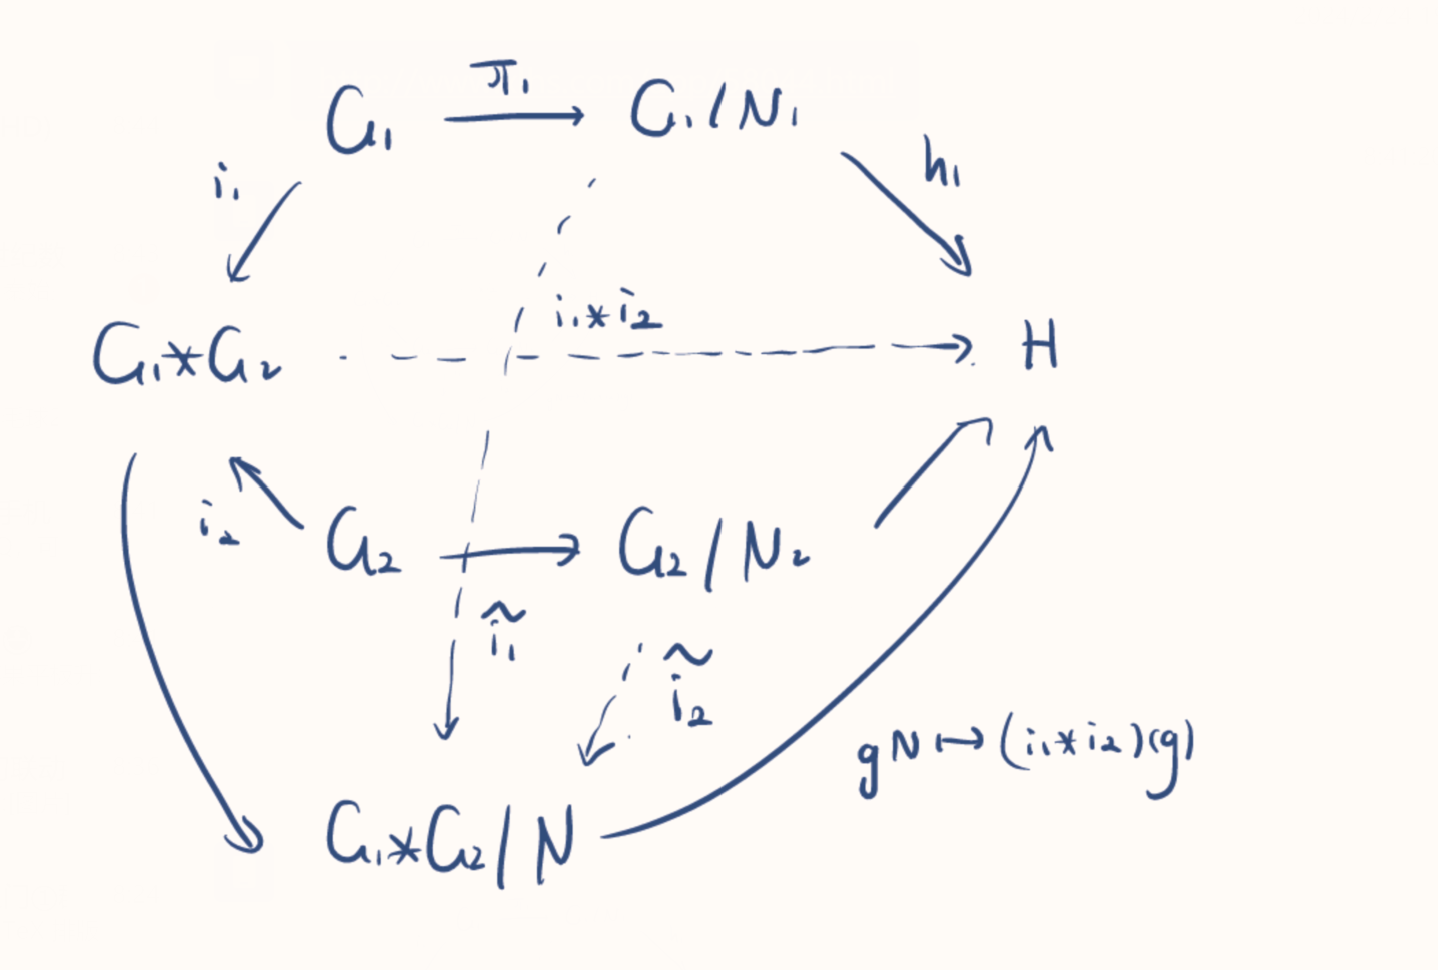
\includegraphics[scale=0.5]{free product.png}
        \centering
    \end{figure}
\end{prooff}

\begin{defn}[free group]
    Let $\left\{a_\alpha\right\}$ be a family of elements of a group $G$. Suppose each $a_\alpha$ generates an infinite cyclic subgroup $G_\alpha$ of $G$. If $G$ is the free product of the groups $\left\{G_\alpha\right\}$, then $G$ is said to be a free group, and the family $\left\{a_\alpha\right\}$ is called a system of free generators for $G$.

    In this case, for each element $x$ of $G$, there is a unique reduced word in the elements of the groups $G_\alpha$ that represents $x$. This says that if $x \neq 1$, then $x$ can be written uniquely in the form
    $$
        x=\left(a_{\alpha_1}\right)^{n_1} \cdots\left(a_{\alpha_k}\right)^{n_k},
    $$
\end{defn}
\begin{defn}
    Let $\left\{a_\alpha\right\}_{\alpha \in J}$ be an arbitrary indexed family. Let $G_\alpha$ denote the set of all symbols of the form $a_\alpha^n$ for $n \in \mathbb{Z}$. We make $G_\alpha$ into a group by defining
    $$
        a_\alpha^n \cdot a_\alpha^m=a_\alpha^{n+m} .
    $$
    Then $a_\alpha^0$ is the identity element of $G_\alpha$, and $a_\alpha^{-n}$ is the inverse of $a_\alpha^n$. We denote $a_\alpha^1$ simply by $a_\alpha$. The external free product of the groups $\left\{G_\alpha\right\}$ is called the free group on the elements $a_\alpha$.
\end{defn}
\begin{theo}
    Given $G$, suppose we are given a family $\left\{a_\alpha\right\}_{\alpha \in J}$ of generators for $G$.
    Let $F$ be the free group on the elements $\left\{a_\alpha\right\}$.
    Then the obvious map $h\left(a_\alpha\right)=a_\alpha$ of these elements into $G$ extends to a homomorphism $h: F \rightarrow G$ that is surjective.
    If $N$ equals the kernel of $h$, then $F / N \cong G$.
    Each element of $N$ is called a relation on $F$, and $N$ is called the relations subgroup. We can specify $N$ by giving a set of generators for $N$.
    But since $N$ is normal in $F$, we can also specify $N$ by a smaller set. Specifically, we can specify $N$ by giving a family $\left\{r_\beta\right\}$ of elements of $F$ such that these elements and their conjugates generate $N$, that is, such that $N$ is
    the least normal subgroup of $F$ that contains the elements $r_\beta$. In this case, we call the family $\left\{r_\beta\right\}$ a complete set of relations for $G$.
\end{theo}


\begin{defn}
    The abelianization $G_{a b}$ of $G$ is the group defined by
    $$
        G_{a b}=G /[G, G],
    $$
    where $[G, G]$ is the (normal) subgroup generated by commutators.
\end{defn}
\begin{prop}
    $f:G\rightarrow H$ is a surjective group homomorphism, $\tilde{f}:G_{ab}\rightarrow H_{ab}$ is the natural homomorphism induced by $f$. Let $i:G\rightarrow G_{ab}$ be the natrual projection.
    Then $\text{Ker}\tilde{f}=i(\text{Ker}f)$
    \label{proposition:quotient,abelianization}
\end{prop}
\begin{exam}
    Consider
    \begin{enu}
        \item $G=\left \langle \,a_1,a_2,\dots ,a_n | a_1^2 \dots a_n^2=e \,\right \rangle $
        \item $H=\left \langle \,a_1,b_1,a_2,b_2\dots,a_n,b_n|[a_1,b_1]\dots[a_n,b_n]=e\,\right \rangle$
    \end{enu}
    Show that $G_{ab}\simeq \bb{Z}^{n-1}\times \bb{Z}/2\bb{Z}$, and $H_{ab}\simeq \bb{Z}^{2n}$
\end{exam}
\begin{prooff}
    For (1), consider the surjective homomorphism $F=F(a_1,\dots,a_n)\rightarrow G$, which induces a surjective homomorphism $\tilde{f}:F_{ab}\rightarrow G_{ab}$.
    Then by Proposition~\ref{proposition:quotient,abelianization}, $G_{ab}$ is isomorphic to $\bb{Z}a_1\oplus \dots \bb{Z}a_n/(2(a_1+\dots+a_n))$.
\end{prooff}

















\newpage
\section{Field Theory}
\subsection{Basic Concept}
\begin{theo}
    Let $p(x) \in F[x]$ be an irreducible polynomial of degree $n$ over the field $F$ and let $K$ be the field $F[x] /(p(x))$. Let $\theta=x \bmod (p(x)) \in K$. Then the elements
    $$
        1, \theta, \theta^2, \ldots, \theta^{n-1}
    $$
    are a basis for $K$ as a vector space over $F$, so the degree of the extension is $n$, i.e., $[K: F]=n$. Hence
    $$
        K=\left\{a_0+a_1 \theta+a_2 \theta^2+\cdots+a_{n-1} \theta^{n-1} \mid a_0, a_1, \ldots, a_{n-1} \in F\right\}
    $$
    consists of all polynomials of degree $<n$ in $\theta$.
\end{theo}
\begin{defn}
    Let $K$ be an extension of the field $F$ and let $S$ be a subset of $K$. Then the smallest subfield of $K$ containing both $F$ and the elements $s\in S$, denoted $F(S)$ is called the field generated by $S$ over $F$.
    If the field $K$ is generated by a single element $\alpha$ over $F, K=F(\alpha)$, then $K$ is said to be a simple extension of $F$ and the element $\alpha$ is called a primitive element for the extension.
\end{defn}
\begin{theo}
    Let $F$ be a field and let $p(x) \in F[x]$ be an irreducible polynomial. Suppose $K$ is an extension field of $F$ containing a root $\alpha$ of $p(x): p(\alpha)=0$. Let $F(\alpha)$ denote the subfield of $K$ generated over $F$ by $\alpha$. Then
    $$
        F(\alpha) \cong F[x] /(p(x))
    $$
    Suppose that $p(x)$ is of degree $n$. Then
    $$
        F(\alpha)=\left\{a_0+a_1 \alpha+a_2 \alpha^2+\cdots+a_{n-1} \alpha^{n-1} \mid a_0, a_1, \ldots, a_{n-1} \in F\right\} \subseteq K
    $$
    \label{theorem:extension by irr polynomial}
\end{theo}
\begin{theo}
    Let $\varphi: F \xrightarrow{\sim} F^{\prime}$ be an isomorphism of fields. Let $p(x) \in F[x]$ be an irreducible polynomial and let $p^{\prime}(x) \in F^{\prime}[x]$ be the irreducible polynomial obtained by applying the map $\varphi$ to the coefficients of $p(x)$. Let $\alpha$ be a root of $p(x)$ (in some extension of $F$ ) and let $\beta$ be a root of $p^{\prime}(x)$ (in some extension of $F^{\prime}$ ). Then there is an isomorphism
    $$
        \begin{aligned}
            \sigma: F(\alpha) & \xrightarrow{\sim} F^{\prime}(\beta) \\
            \alpha            & \longmapsto \beta
        \end{aligned}
    $$
    mapping $\alpha$ to $\beta$ and extending $\varphi$, i.e., such that $\sigma$ restricted to $F$ is the isomorphism $\varphi$.
    \label{theorem:extend simple extenison}
\end{theo}

\vskip 1cm
In the following statements, we always assume $F$ be a field and let $K$ be an extension of $F$, $\alpha,\beta\in K$ be an element.
\begin{defn}
    The element $\alpha \in K$ is said to be algebraic over $F$ if $\alpha$ is a root of some nonzero polynomial $f(x) \in F[x]$. If $\alpha$ is not algebraic over $F$, then $\alpha$ is said to be transcendental over $F$. The extension $K / F$ is said to be algebraic if every element of $K$ is algebraic over $F$.

    Let $\alpha$ be algebraic over $F$. Then there is a unique monic irreducible polynomial $m_{\alpha, F}(x) \in F[x]$ which has $\alpha$ as a root. A polynomial $f(x) \in F[x]$ has $\alpha$ as a root if and only if $m_{\alpha, F}(x)$ divides $f(x)$ in $F[x]$.
\end{defn}
\begin{theo}
    Let $\alpha$ be algebraic over the field $F$ and let $F(\alpha)$ be the field generated by $\alpha$ over $F$. Then
    $$
        F(\alpha) \cong F[x] /\left(m_\alpha(x)\right)
    $$
    so that in particular
    $$
        [F(\alpha): F]=\operatorname{deg} m_\alpha(x)=\operatorname{deg} \alpha,
    $$
    i.e., the degree of $\alpha$ over $F$ is the degree of the extension it generates over $F$.
\end{theo}
\begin{prop}
    The element $\alpha\in K$ is algebraic over $F$ if and only if the simple extension $F(\alpha) / F$ is finite. More precisely, if $\alpha$ is an element of an extension of degree $n$ over $F$ then $\alpha$ satisfies a polynomial of degree at most $n$ over $F$ and if $\alpha$ satisfies a polynomial of degree $n$ over $F$ then the degree of $F(\alpha)$ over $F$ is at most $n$.
\end{prop}
\begin{defn}
    Let $K_1$ and $K_2$ be two subfields of a field $K$. Then the composite field of $K_1$ and $K_2$, denoted $K_1 K_2$, is the smallest subfield of $K$ containing both $K_1$ and $K_2$. Similarly, the composite of any collection of subfields of $K$ is the smallest subfield containing all the subfields.
\end{defn}
\begin{prop}
    $F(\alpha,\beta)=(F(\alpha))(\beta)$, i.e., the field generated over $F$ by $\alpha$ and $\beta$ is the field generated by $\beta$ over the field $F(\alpha)$ generated by $\alpha$. In general, if $a_1,\dots,a_n$ be elements of $K$, then $F(a_1,\dots,a_n)=((F(a_1)(a_2))\dots)(a_n)$
\end{prop}
\begin{coro}
    If $K\subset L\subset M$ are field extensions, $L/K,M/L$ are algebraic extensions, then $M/K$ is algerbaic.
    \label{corollary:algebraic extension is transitive}
\end{coro}
\begin{defn}[spilting field]
    The extension field $K$ of $F$ is called a splitting field for the polynomial $f(x) \in F[x]$ if $f(x)$
    factors completely into linear factors (or splits completely) in $K[x]$ and $f(x)$ does not factor completely into linear factors over any proper subfield of $K$ containing $F$.
\end{defn}
\begin{theo}
    For any field $F$, if $f(x) \in F[x]$ then there exists an extension $K$ of $F$ which is a splitting field for $f(x)$.
\end{theo}
\begin{prooff}
    We first show that there is an extension $E$ of $F$ over which $f(x)$ splits completely into linear factors by induction on the degree $n$ of $f(x)$. If $n=1$, then take $E=F$. Suppose now that $n>1$. If the irreducible factors of $f(x)$ over $F$ are all of degree 1 , then $F$ is the splitting field for $f(x)$ and we may take $E=F$. Otherwise, at least one of the irreducible factors, say $p(x)$ of $f(x)$ in $F[x]$ is of degree at least 2 . Hence, there is an extension $E_1$ of $F$ containing a root $\alpha$ of $p(x)$. Over $E_1$ the polynomial $f(x)$ has the linear factor $x-\alpha$. The degree of the remaining factor $f_1(x)$ of $f(x)$ is $n-1$, so by induction there is an extension $E$ of $E_1$ containing all the roots of $f_1(x)$. Since $\alpha \in E, E$ is an extension of $F$ containing all the roots of $f(x)$. Now let $K$ be the intersection of all the subfields of $E$ containing $F$ which also contain all the roots of $f(x)$. Then $K$ is a field which is a splitting field for $f(x)$.
\end{prooff}
\begin{defn}
    The field $\bar{F}$ is called an algebraic closure of $F$ if $\bar{F}$ is algebraic over $F$ and if every polynomial $f(x) \in F[x]$ splits completely over $\bar{F}$ (so that $\bar{F}$ can be said to contain all the elements algebraic over $F$ ).

    A field $K$ is said to be algebraieally closed if every polynomial with coefficients in $K$ has a root in $K$.
\end{defn}
\begin{theo}
    Let $\bar{F}$ be an algebraic closure of $F$. Then $F$ is algebraically closed.
\end{theo}
\begin{prooff}
    By Corollary~\ref{corollary:algebraic extension is transitive}.
\end{prooff}
\begin{lem}[extension of $F$-homomorphism for algebraic extension]
    Let $\varphi: F \xrightarrow{\sim} F^{\prime}$ be an isomorphism of fields, $\bar{F\p}$ be the algebraic closure of $F\p$, $E/F$ is a algebraic extension, then there's $\sigma:E\rightarrow \bar{F\p}$ ring homomorphism satisfying $\sigma|_{F}=\varphi$.
    \label{lemma:extend algebraic extension}
\end{lem}
\begin{prooff}
    By Zorn's Lemma and Theorem~\ref{theorem:extend simple extenison}.
\end{prooff}
\begin{theo}
    For any field $F$, algebraic closure of $F$ exists and is unique up to isomorphism.
\end{theo}
\begin{prooff}
    Existence: For each polynomial $f \in F[X]$, choose a splitting field $E_f$, and let $$\Omega=\left(\bigotimes_{f\in F[x]} E_f\right) / M$$ where $M$ is a maximal ideal. It is clear that $\Omega$ is a $F$-algebra and $E_f$ can be embedded into $\Omega$. Since $f$ splits in $E_f$, it must also split in the larger field $\Omega$. Then all the algebraic elements in $\Omega$ is therefore an algebraic closure of $F$.

    Uniqueness: By Lemma~\ref{lemma:extend algebraic extension}.

\end{prooff}
\subsection{Separable}
In the following statements, $F$ is a field, and we fix an algebraic closure of $F$ and denote it by $\bar{F}$.
\begin{defn}[separable]
    A polynomial $f(x)\in F[x]$ is separable if $f(x)$ has no multiple root in $\bar{F}$.
\end{defn}
\begin{prop}
    A polynomial $f(x)$ has a multiple root $\alpha\in \bar{F}$ if and only if $\alpha$ is also a root of $f\p(x)$. In particular, $f(x)$ is separable if and only if it is relatively prime to its derivative: $\left(f(x), D_x f(x)\right)=1$.
    \label{proposition: criterion for separable polynomial}
\end{prop}
\begin{rema}
    For any two polynomials $f(x),g(x)\in F[x]$, they have the same g.c.d in $F[x]$ and $\bar{F}[x]$ since Euclidean division doesn't change if we replace $F$ by any extension field of $F$.
\end{rema}

\begin{defn}
    $\alpha\in \bar{F}$ is separable if $m_{\alpha}(x)\in F[x]$ is separable polynomial.

    $F\subset E\subset \bar{F}$ are field extensions, $E/F$ is a separable extension if for all $\alpha \in E$, $\alpha$ is separable.
\end{defn}



\begin{defn}[perfect field]
    A field $F\subset \bar{F}$ is perfect if and only if every finite extension of $F$ is separable.
\end{defn}
\begin{lem}
    Let $p(x)$ be an irreducible polynomial over a field $F$ of characteristic $p$. Then there is a unique integer $k \geq 0$ and a unique irreducible separable polynomial $p_{\text {sep }}(x) \in F[x]$ such that
    $$
        p(x)=p_{sep}\left(x^{p^k}\right)
    $$
    Hence $p(x)=\deg p_{sep}p^k$
    and $\deg p_{sep}$ is called the separable degree, $p^k$ is called the inseparable degree of $P$.
    \label{lemma:p(x)=psep(x^p^k)}
\end{lem}
\begin{prop}
    A field $F$ is perfect if and only if it is a field of characteristic $0$ or a field of characteristic $p>0$ such that every element has a $p$-th root.
\end{prop}
\begin{prooff}
    '$\Longleftarrow$':
    case 1: If $\text{chap}\, F=0$, then by Proposition~\ref{proposition: criterion for separable polynomial}, $F$ is perfect.

    case 2: If $\text{chap}\, F=p$, $\alpha\in \bar{F}$, and $p(x)=m_{\alpha}(x)\in F[x]$ is inseparable, by Lemma~\ref{lemma:p(x)=psep(x^p^k)}, there's irreducible polynomial $q(x)$ such that $p(x)=q(x^p)$.
    Hence $$p(x)=a_m x^{pm}+\dots+ a_1 x^{p}+a_0=b^p_m x^{pm}+\dots b^p_1 x^{p}+b_0^p=(b_mx^m+\dots b_0)^p$$
    where $b_i^p=a_i$ for $i=0,\dots m$. A contradiction!

    '$\Longrightarrow$': if $\text{chap}\, F=p$ and $\alpha\in \bar{F}$ is not a $p$-th root, consider $p(x)=x^p-\alpha$. Notice that $(p(x),p\p(x))=p(x)$, then $p(x)$ is inseparable. However, if $\beta\in \bar{F}$ is a root of $p(x)$, then $p(x)=x^p-\alpha=x^p-\beta^p=(x-\beta)^p$.
    If $p(x)$ is reducible in $F[x]$, $p(x)=a(x)b(x)$ where $\deg a(x),\deg b(x)<p$.

    Notice that $a(x)=(x-\beta)^{s},b(x)=(x-\beta)^{t}\in F[x]$ with $s+t=p$, then $\beta^s\in F,\beta^t\in F$. Hence by Bezout Theorem, we have $\beta^{(s,t)}=\beta\in F$ which contradict to the fact that $\alpha$ is not a $p$-th root. Hence $p(x)$ is irreducible inseparable polynomial, and contradict to the fact $F$ is perfect!
\end{prooff}

\begin{coro}
    In the proof of above Proposition, we can obtain if $\text{chap}\, F\neq 0$ and $p(x)=x^p-\alpha\in F[x]$, either $p(x)$ is irreducible or $p(x)=(x-\beta)^p$ for some $\beta\in F$.
\end{coro}
\begin{exam}
    $\bb{Q},\bb{F}_q$ are perfect fields and $\bb{F}_p(t)$ is not perfect field.
\end{exam}
\begin{defn}
    Given field extensions $F\subset E\subset \bar{F}$, $E$ is called purely inseparable if for each $\alpha \in E$ the minimal polynomial of $\alpha$ over $F$ has only one distinct root.
    It is easy to see that the following are equivalent:
    \begin{enumerate}[(1)]
        \item $E / F$ is purely inseparable
        \item if $\alpha \in E$ is separable over $F$, then $\alpha \in F$
        \item if $\alpha \in E$, then $\alpha^{p^n} \in F$ for some $n$ (depending on $\alpha$ ), and $m_{\alpha, F}(x)=x^{p^n}-\alpha^{p^n}$.
    \end{enumerate}
    \label{Definition:characterizations of purely inseparable}
\end{defn}
\begin{prop}
    Given a field extension $K/F, u \in K$ is separable over $F$ iff $F(u)=$ $F\left(u^p\right)$.
    \label{lemma:Fu=Fup}
\end{prop}
\begin{prooff}
    We assume $u$ is separable first. Then $F_1=F\left(u^p\right) \subseteq F(u)$. Consider the polynomial $X^p-u^p \in F_1[X]$ and $u$ is a root of it. Let $P$ be the minimal polynomial of $u$ over $F_1 \Rightarrow P \mid X^p-u^p$. But $X^p-u^p=(X-u)^p$. Thus $P=(X-u)^k$ for some integer $k$. Since $P$ is separable and all roots of it are different, $P=X-u$. Hence $u \in F_1$. Then $F(u)=F\left(u^p\right)$.

    On the other hand, we assume $F(u)=F\left(u^p\right)$.
    Let $P$ be the minimal polynomial of $u$ over $F$. If $P$ is not separable, then $P(X)=P_1\left(X^p\right)$. Since $P_1$ is irreducible and $P\left(u^p\right)=0, P_1$ is the minimal polynomial of $u^p$. Then $[F(u): F]=\left[F\left(u^p\right): F\right]=\operatorname{deg} P=\operatorname{deg} P_1=p \cdot \operatorname{deg} P_1$. A contradiction! Hence $P$ is separable and $u$ is separable.
\end{prooff}
\begin{prop}
    Assume $[K: F]=d<\infty$. The following statements are equivalent.
    \begin{enu}
        \item $F \subseteq K$ is separable.
        \item $K=F \cdot K^p$, where $K^p=\left\{k^p \mid k \in K\right\}$ a subfield of $K$ since $\operatorname{char}(F)=\operatorname{char}(K)=$ $p>0$;
        \item  There is a basis $\left\{e_1, \ldots, e_d\right\}$ of $K$ over $F$ such that $\left\{e_1^p, \ldots, e_d^p\right\}$ is still a basis.
    \end{enu}
    \label{lemma:equivalent def of separable extenison}
\end{prop}
\begin{prop}
    A simple algebraic extension $F(u)/F$ is separable iff $u$ is separable over $F$.
\end{prop}
\begin{prooff}
    If $P(X) \in$ $F[X]$ is the minimal polynomial of $u$ over $F, P(X)=\sum_k a_k X^k$
    with $\operatorname{deg}(P)=n$, then $\left\{1, u, \ldots, u^{n-1}\right\}$ form a
    basis of $F(u)$ over $F$. We prove $\left\{1, u^p, \ldots, u^{p(n-1)}\right\}$ is a basis as well.

    If this is true, from the Lemma~\ref{lemma:equivalent def of separable extenison},
    $F(u)/F$ is separable.

    If this is not true, there will exist $\left\{b_k\right\}$ which are not all zero
    such that $\sum_k b_k u^{k p}=0$.
    Let $P_1(X)=\sum_k b_k X^k$, with $\operatorname{deg}\left(P_1\right) \leq n-1$. $P_1\left(u^p\right)=0$. Then $\left[F\left(u^p\right): F\right] \leq \operatorname{deg}\left(P_1\right) \leq$ $n-1$.
    But since $u$ is separable, $F(u)=F\left(u^p\right),[F(u)$ : $F]=\left[F\left(u^p\right): F\right]=n$, a contradiction!
\end{prooff}
\begin{prop}
    $F \subseteq E \subseteq K$ are field extensions. $K / F$ is separable iff $E / F$ and $K / E$ are separable.
\end{prop}
\begin{prooff}
    We only prove the part of $\Leftarrow$. If $[K: F]<\infty$, $K=E \cdot K^p=\left(F \cdot E^p\right) \cdot K^p=F \cdot\left(E^p \cdot K^p\right)=F \cdot K^p$. Hence $K / F$ is separable.

    If $[K: F]=\infty, u \in K$ and $P_u \in E[X]$ is the minimal polynomial of $u$ over $E$. $P_u(X)=X^n+a_{n-1} X^{n-1}+\ldots+a_0$. Consider $F \subseteq F\left(a_0, \ldots, a_{n_1}\right) \subseteq E \subseteq E(u) \subseteq K$.
    Since $E / F$ is separable, according to the part of $\Rightarrow$ of 1 ., we know $F\left(a_0, \ldots, a_{n-1}\right) / F$ is separable.
    And since the minimal polynomial of $u$ over $F\left(a_0, \ldots, a_{n_1}\right)$ is just $P_u$,
    which is separable. Then $F\left(a_0, \ldots, a_{n_1}, u\right) / F\left(a_0, \ldots, a_{n_1}\right)$ is separable. Since $\left[F\left(a_0, \ldots, a_{n_1}, u\right): F\right]<\infty, F\left(a_0, \ldots, a_{n_1}, u\right) / F$ is separable and especially $u$ is separable.
\end{prooff}
\begin{defn}
    Given an algebraic extension $K / F$, all separable elements in $K$ form a subfield containing $F$, which is denoted by $K_s$. Especially if $K=\bar{F}, \bar{F}_s$ is denoted by $F_{s e p}$ and called the separable closure. This motivates us to study $K_s / F$ and $K / K_s$ respectively, which is the task in the next subsection.
\end{defn}
\begin{prop}
    If $E / F$ and $E^{\prime} / F$ are separable, then $E \cdot E^{\prime} / F$ is separable.
\end{prop}
\begin{prop}
    Given a finite algebraic extension $K / F$, we have the following equation
    $$
        [K: F]_s=\left|\operatorname{Hom}_F(K, \bar{F})\right|
    $$
\end{prop}
More generally, we have
\begin{coro}
    Let $\varphi: F \xrightarrow{\sim} F^{\prime}$ be an isomorphism of fields, $\bar{F\p}$ be the algebraic closure of $F\p$,
    $E/F$ is a finite separable extension, then there are exactly $[E:F]$ ways to give an extension
    $\sigma:E\rightarrow \bar{F\p}$ ring homomorphism satisfying $\sigma|_{F}=\varphi$.

    \label{lemma:extend simple extension}
\end{coro}
\subsection{Normal}
\begin{defn}
    Let $F\subset E\subset \bar{F}$ be field extensions, we call $E/F$ normal if for all $\alpha\in E$, all the roots of $m_{\alpha}(x)$ lie in $E$.
\end{defn}
\begin{defn}
    Let $F\subset E\subset \bar{F}$ be field extensions. Let $\text{Aut}(E/F)$ be the collection of
    automorphisms of $K$ which fix $F$.
\end{defn}
\begin{theo}
    Let $F\subset E\subset \bar{F}$ be field extensions, the following statements are equivalent:
    \begin{enumerate}[(1)]
        \item $E/F$ is normal.
        \item every $F$-algebra homomorphism from $E$ to $\bar{F}$ is a $F$-algebra homomorphism from $E$ to $E$.
    \end{enumerate}
    Moreover, if $[E: F]<\infty$, then the above statements are equivalent to that $E$ is a splitting field of some $p(x) \in F[x]$.
    \label{theorem:characterizations of normal extension}
\end{theo}
\begin{prooff}
    (1)$\Longrightarrow $(2) is clear.

    (2)$\Longrightarrow $(1): By Lemma~\ref{lemma:extend algebraic extension}

    Now suppose $[E: F]<\infty$. First we assume $F \subseteq E$ is normal and choose $u_1 \in E-F$. Then its minimal polynomial is $P_{u_1}$ and $\left[E: F\left(u_1\right)\right]<[E: F]$. Next we choose $u_2 \in E-F\left(u_1\right)$. Continuing this process, we conclude $E=F\left(u_1, \ldots, u_n\right)$. Let $P=\prod_{i=1}^n P_{u_i}$, and then $E$ is the splitting field of $P$.

    On the other hand, if $E$ is the splitting field of $P \in F[X]$ whose roots in $\bar{F}$ are $\left\{u_1, \ldots, u_n\right\}$. Then $E=F\left(u_1, \ldots, u_n\right)$. Consider an $F$-algebra homomorphism $\iota: F\left(u_1, \ldots, u_n\right) \rightarrow$ $\bar{F}$, since $\iota\left(u_i\right)$ is a root of $P$ as well, $\iota\left(u_i\right) \in E$. Hence $\iota(E) \subseteq E$.

\end{prooff}

\begin{prop}
    Given field extensions $F\subset E\subset \bar{F}$, then all $F$-algerba homomorphisms from $E$ to $E$ are in $\text{Aut}(E/F)$ i.e. $\text{Aut}(E/F)={\bbrace{ F\text{-algebra homomorphism between } E \text{ and } E  }}$
    \label{proposition:F algebra hom is surjective}
\end{prop}
\begin{prooff}
    Given any $F$-algebra homorphism $\tau: E \rightarrow E$,
    we know it's injective and it' enough to prove it's surjective.
    We assume $u \in E$ and $P \in F[x]$ is its minimal polynomial over $F$. If $u_1, \ldots, u_n$ are its different roots in $\bar{F}$, we assume only $u_1, \ldots, u_r$ are in $E$. Then $u \in\left\{u_1, \ldots, u_r\right\}$.
    Since $\tau$ fixes $F, \tau\left(u_i\right)$ is also a root of $P$ in $E$ where $1 \leq i \leq r$.
    Then $\tau:\left\{u_1, \ldots, u_r\right\} \rightarrow\left\{u_1, . ., u_r\right\}$. That $\tau$ is injective implies it's surjective on this subset as well, which means $\exists u_i, \tau\left(u_i\right)=u$.
\end{prooff}
\begin{prop}
    For field extensions $F \subseteq E \subseteq K \subseteq \bar{F}$, if $K / F$ is normal then $K / E$ is normal.
\end{prop}
\begin{prop}
    If $E / F$ and $E^{\prime} / F$ are normal, then $E \cdot E^{\prime} / F$ is normal.
\end{prop}
\subsection{Galios}
\begin{defn}
    Let $E/F$ be a finite extension. Then $E$ is said to be Galois over $F$ and $E/F$ is a Galois extension if it is separable and normal.
\end{defn}
\begin{theo}[Fundamental Theorem of Galois Theory]
    $F\subset K\subset \bar{F}$ be field extensions. $K / F$ be a Galois extension and set $G=\operatorname{Gal}(K / F)$. Then there is a bijection:
    \begin{equation*}
        \bbrace{\text{subfield of } K \text{ containing } F }\longleftrightarrow \bbrace{\text{subgroup of } G }
    \end{equation*}
    given by the correspondences
    % https://q.uiver.app/#q=WzAsNCxbMCwwLCJFIl0sWzIsMCwiXFxsZWZ0XFx7XFx0ZXh0e2VsZW1lbnRzIG9mIH0gRyBcXHRleHR7IGZpeGluZyB9IEUgIFxccmlnaHRcXH0iXSxbMiwxLCJIIl0sWzAsMSwiXFx0ZXh0e2ZpeCBmaWVsZCBvZiB9IEgiXSxbMCwxXSxbMiwzXV0=
    \[\begin{tikzcd}
            E && {\left\{\text{elements of } G \text{ fixing } E  \right\}} \\
            {\text{fix field of } H} && H
            \arrow[from=1-1, to=1-3]
            \arrow[from=2-3, to=2-1]
        \end{tikzcd}\]
    which are inverse to each other. Under this correspondence,
    \begin{enumerate}[(1)]
        \item $K/E$ is always Galois.
        \item there's a one-to-one correspondence:
              % https://q.uiver.app/#q=WzAsMyxbMCwwLCJcXEJpZ2dcXHsgRlxcdGV4dHstYWxnZWJyYSBob21vbW9ycGhpc219XFx0ZXh0e2JldHdlZW4gfSBFIFxcdGV4dHsgYW5kIH0gXFxiYXJ7Rn0gIFxcQmlnZ1xcfSJdLFswLDIsIlxcbGVmdFxce1xcdGV4dHtsZWZ0IGNvc2V0cyBvZiB9IEggXFx0ZXh0eyBpbiB9IEdcXHJpZ2h0XFx9Il0sWzIsMiwiXFxsZWZ0XFx7ICBcXHNpZ21hfF9FOlxcc2lnbWFcXGluIEc6ICAgXFxyaWdodFxcfSJdLFsxLDAsIlxcc2lnbWEgSFxcbWFwc3RvIFxcc2lnbWF8X0UiLDJdLFsxLDIsIlxcc2lnbWEgSFxcbWFwc3RvIFxcc2lnbWF8X0UiXSxbMCwyLCJcXHRleHR7RXh0ZW5kZWQgYnkgVGhlb3JlbX1+XFxyZWZ7fSJdXQ==
              \[\begin{tikzcd}
                      {\bbrace{ F\text{-algebra homomorphism between } E \text{ and } \bar{F}  }} \\
                      \\
                      {\left\{\text{left cosets of } H \text{ in } G\right\}} && {\left\{  \sigma|_E:\sigma\in G   \right\}}
                      \arrow["{\sigma H\mapsto \sigma|_E}"', from=3-1, to=1-1]
                      \arrow["{\sigma H\mapsto \sigma|_E}", from=3-1, to=3-3]
                      \arrow["{\text{Extended by}~\ref{lemma:extend algebraic extension}\text{ and }\ref{proposition:F algebra hom is surjective}}", from=1-1, to=3-3]
                  \end{tikzcd}\]
        \item (inclusion reversing) If $E_1, E_2$ correspond to $H_1, H_2$, respectively, then $E_1 \subseteq E_2$ if and only if $H_2 \leq H_1$
        \item $[K: E]=|H|$ and $[E: F]=[G: H]$
        \item For all $\sigma\in G$,$$\sigma(E)\longleftrightarrow \sigma H\sigma^{-1}$$
              In particular, by Theorem~\ref{theorem:characterizations of normal extension}, $E$ is normal(hence Galois) over $F$ if and only if $H$ is a normal subgroup in $G$. If this is the case, then the Galois group is isomorphic to the quotient group
              $$
                  \operatorname{Gal}(E / F) \cong G / H
              $$
        \item If $E_1, E_2$ correspond to $H_1, H_2$, respectively, then the intersection $E_1 \cap E_2$ corresponds to the group $\left(H_1, H_2\right.$ ) generated by $H_1$ and $H_2$ and the composite field $E_1 E_2$ corresponds to the intersection $H_1 \cap H_2$.
    \end{enumerate}

\end{theo}
In the following statements, we fix a algebraic closure of $F$, and $K,F\p,K_1,K_2$ containing $F$ are subfield of $\bar{F}$.
\begin{theo}
    Suppose $K/F$ is a Galois extension and $F^{\prime} / F$ is any extension. Then $K F^{\prime} / F^{\prime}$ is a Galois extension, with Galois group
    $$
        \operatorname{Gal}\left(K F^{\prime} / F^{\prime}\right) \cong \operatorname{Gal}\left(K / K \cap F^{\prime}\right)
    $$
    isomorphic to a subgroup of $\operatorname{Gal}(K / F)$.
\end{theo}
\begin{coro}
    Suppose $K / F$ is a Galois extension and $F^{\prime} / F$ is any finite extension. Then
    $$
        \left[K F^{\prime}: F\right]=\frac{[K: F]\left[F^{\prime}: F\right]}{\left[K \cap F^{\prime}: F\right]}
    $$
\end{coro}
\begin{theo}
    Let $K_1$ and $K_2$ be Galois extensions of a field $F$. Then
    \begin{enumerate}[(1)]
        \item The intersection $K_1 \cap K_2$ is Galois over $F$.
        \item The composite $K_1 K_2$ is Galois over $F$. The Galois group is isomorphic to the subgroup
              $$
                  H=\left\{(\sigma, \tau)|\sigma|_{K_1 \cap K_2}=\left.\tau\right|_{K_1 \cap K_2}\right\}
              $$
              of the direct product $\operatorname{Gal}\left(K_1 / F\right) \times \operatorname{Gal}\left(K_2 / F\right)$ consisting of elements whose restrictions to the intersection $K_1 \cap K_2$ are equal.
    \end{enumerate}
\end{theo}
\begin{coro}
    $F\subseteq E \subseteq F_{sep}\subseteq \bar{F}$ be finite separable extension, there's Galois extension $K_1$ contains $E$(for example, the composite of the splitting fields of the minimal polynomials for a basis for $E$ over $F$). Take $S$ be the set of all the Galois extenison of $F$ which contains $E$, then
    \begin{equation*}
        \bar{E}=\bigcap_{K\in S} K =\bigcap_{K\in S} (K\cap K_1)
    \end{equation*}
    is acturally finite many intersection of Galois extenison of $F$ which contains $E$ by Fundamental Theorem of Galois Theory.

    Hence, there's minimal Galois extension of $F$ that contains $E$.
\end{coro}
\begin{coro}
    If $K/F$ is finite and separable, then $K / F$ is simple. In particular, any finite extension of fields of characteristic 0 is simple.
\end{coro}
\begin{prop}
    $\bar{F}/F_{sep}$ is pruely inseparable extension and $F_{sep}$ is separable and normal extension.
\end{prop}
\begin{prooff}
    By characterizations of purely inseparable extension and definition of normal extension.
\end{prooff}
\begin{defn}
    \item A subset $\left\{a_1, a_2, \ldots, a_n\right\}$ of $E$ is called algebraically independent over $F$ if there is no nonzero polynomial
    $$
        f\left(x_1, x_2, \ldots, x_n\right) \in F\left[x_1, x_2, \ldots, x_n\right]
    $$
    such that $f\left(a_1, a_2, \ldots, a_n\right)=0$. An arbitrary subset $S$ of $E$ is called algebraically independent over $F$ if every finite subset of $S$ is algebraically independent. The elements of $S$ are called independent transcendentals over $F$.

    \item A transcendence base for $E / F$ is a maximal subset (with respect to inclusion) of $E$ which is algebraically independent over $F$.

    \item The extension $E / F$ has a transcendence base and any two transcendence bases of $E / F$ have the same cardinality.
\end{defn}
\begin{defn}
    The cardinality of a transcendence base for $E / F$ is called the transcendence degree of $E / F$.
\end{defn}
\begin{prop}
    $E/F$ be a field extension, $\alpha_1,\dots,\alpha_n\in E$, $F_i=F(a_1,\dots,a_i)$, then $\bbrace{\alpha_1,\dots,\alpha_n}$ is algebracally independent over $F$, if and only if $\alpha_{i}$ is transcendental over $F_{i-1}$ for all $i=1,\dots,n$.
    \label{proposition:transcendental extension, renumber}
\end{prop}




\chapter{Commutative Algebra}
\section{Basic Definition in Ring Thoery}
\begin{defn}
    A zero-divisor in a ring $A$ is an element $x$ which "divides 0", i.e., for which there
    exists $y\neq 0$ in A such that $xy = 0$.
\end{defn}
\begin{defn}
    An ideal which is maximal among all proper ideals is called a maximal
    ideal; an ideal $m$ of $A$ is maximal if and only if $A/m$ is a field.
\end{defn}
\begin{theo}
    If $I$ is a proper ideal then there exists at least one maximal
    ideal containing $I$.
\end{theo}
\begin{defn}
    A ring A is an integral domain (or simply a
    domain) if $ A\neq 0$, and $A$ has no zero-divisors other than 0.
\end{defn}
\begin{defn}
    A field $F$ is an integral doamin such that every non-zero element in $F$ is invertible.
\end{defn}

\begin{defn}
    A proper ideal($\neq A$) $P$ of $A$ for which $A/P $ is an integral domain is called a prime
    ideal. In other words, $P$ is prime if it satisfies:
    \begin{enumerate}[(1)]
        \item $ P\neq A$.
        \item $x,y \in Р \Rightarrow xy \in P$ for $x,y\in A$.
    \end{enumerate}
    A field is an integral domain, so that a maximal ideal is prime.
\end{defn}
\begin{prop}
    There is a one-to-one order-preserving correspondence
    between the ideals $J$ of $A$ which contain $I$, and the ideals $A/I$.More precisely,we can say
    there are two bijection
    \begin{equation*}
        \bbrace{\text{ideals of A that contain I}}\longleftrightarrow \bbrace{\text{ideals of } A/I}
    \end{equation*}
    \begin{equation*}
        \bbrace{\text{prime ideals of A that contain I}}\longleftrightarrow \bbrace{\text{prime ideals of } A/I}
    \end{equation*}
    given by the correspondences
    \begin{equation*}
        J  \longrightarrow  J/I=\bar{J}
    \end{equation*}
    \begin{equation*}
        \pi^{-1}(\bar{J})  \longleftarrow \bar{J}
    \end{equation*}
    where $\pi$ be the natural homomorphism from $A$ to $A/I$.
\end{prop}
\begin{defn}
    A subset $S$ of $A$ is multiplicative if it satisfies:
    \begin{enumerate}[(1)]
        \item $x,y\in S \Rightarrow xy \in S$.
        \item $1 \in S$.
    \end{enumerate}
\end{defn}
\begin{defn}
    If $I$ is an ideal of $A$ then the set of elements of $A$, some power of which
    belongs to $I$, is an ideal of $A$.This set is called the radical of $I$, and is sometimes written $\sqrt{I}$.
\end{defn}
\begin{theo}
    the radical $\sqrt{I}$ of $I$ is the interchapter of all prime ideals containing $I$.
\end{theo}
\begin{prooff}
    \begin{lem}
        Let $S$ be a multiplicative set and $I$ an ideal disjoint from $S$;
        then there exists a prime ideal containing $I$ and disjoint from $S$.
        \label{lemma:multiplicative set,prime ideal}
    \end{lem}
    \begin{proofff}
        If $I$ is an ideal disjoint from $S$,then the set of ideals containing $I$ and disjoint from $S$ has a maximal
        element. If $P$ is an ideal which is maximal among ideals disjoint from $S$
        then $P$ is prime. For if $x,y\notin P,xy\in P$, then since $P+xA$ and $P+yA$ both
        meet $S$, the product $(P + xA) (P + y A)$ also meets $S$. However,
        $(P + xA) (P + y A) \subset P+xyA$ ,a contradiction!
    \end{proofff}
    If $x\notin \sqrt{I}$, $S_x={x^n:n\ge 0}$ be a multiplicative subset. By lemma~\ref{lemma:multiplicative set,prime ideal}, we can find
    a prime ideal which contains $I$ disjoint from $S_x$.
\end{prooff}
\begin{defn}
    In particular if we take $I = (0)$ then $\sqrt{(0)}$ is the set of all nilpotent elements
    of $A$, and is called the nilradical of $A$; we will write $nil(A)$ for this. When $nil(A) = 0$ we say
    that $A$ is reduced, For any ring $A$ we write $A_{red}$ for $A/nil(A)$ is of course reduced.
\end{defn}
\begin{defn}
    The interchapter of all maximal ideals of a ring $A\neq 0$ is called the
    Jacobson radical, or simply the radical of $A$ and written $rad(A)$.
\end{defn}
\begin{prop}
    $x\in rad(A)$ if and only if $1+xy$ is a unit in $A$ for all $y\in A$.
    \label{proposition:Jacobson radical}
\end{prop}
\begin{defn}
    A ring having just one maximal ideal is called a local ring, and a
    (non-zero) ring having only finitely many maximal ideals a semilocal ring.
    We often express the fact that $A$ is a local ring with maximal ideal $m$ by
    saying that $(A, m)$ is a local ring; if this happens then the field $k = A/m$ is
    called the residue field of $A$. We will say that $(A,m,k)$ is a local ring to
    mean that A is a local ring, $m = rad(A)$ and $k = A/m$.
\end{defn}
\begin{prop}
    If $(A,m)$ is a local ring then the elements of $A$ not contained in $m$ are units; conversely a
    (non-zero) ring $A$ whose non-units form an ideal $m$ is a local ring with maximal ideal $m$.
    \label{Proposition:unit=A-m}
\end{prop}
\begin{theo}
    If $I_1,I_2,...,I_n$ are ideals which are coprime(i.e. $I_i+I_j=A$ for all $i\neq j$) in pairs then
    $I_1 I_2\dots I_n=I_1\cap I_2\dots \cap I_n$
\end{theo}
\begin{theo}[Chinese Reminder Theorem]
    If $I_1,\dots, I_n$ are ideals which are coprime in pairs then
    \begin{equation*}
        A/I_1\times \dots \times A/I_n\simeq A/(I_1\dots I_n)
    \end{equation*}
    and the isomorphism map is given by
    \begin{equation*}
        a+I_1\dots I_n\rightarrow (a+I_1,\dots,a+I_n)
    \end{equation*}
\end{theo}
\begin{theo}[Prime Avoidance]
    \par
    \begin{enumerate}[(1)]
        \item Let $P_1,\dots P_n$ be prime ideals and let $I$ be an ideal
              contained in $\bigcup_{i=1}^n P_i$. Then $I\subset P_i$ for some $1 \le i \le n$.
        \item Let $P$ be a prime ideal. $P\supset I_1\dots I_n$, then $P\supset I_i$ for some $1\le i \le n$.
    \end{enumerate}
    \label{theorem:prime avoidance}
\end{theo}
\begin{prooff}
    (2):If $P\supset IJ$ and $P\nsupseteq I$, there's $a\in I$ such that $a\notin P$. Since $P\supset IJ$, for all $b\in J$, $ab\in P$, then $b\in P$. Hence we have $P\supset J $.
\end{prooff}
\begin{defn}
    Let $R$ be an integral domain.
    Suppose $r\in R$ is nonzero and is not a unit. Then $r$ is called irreducible in $R$
    if whenever $r = ab$ with $a, b\in R$, at least one of $a$ or $b$ must be a unit in $R$.
    Otherwise $r$ is said to be reducible.The nonzero element $p\in R$ is called prime in $R$ if the ideal $(p)$ generated by
    $p$ is a prime ideal.Two elements $a$ and $b$ of $R$ differing by a unit are said to be associate in $R$.
\end{defn}
\begin{prop}
    In an integral domain, a prime element is always irreducible.
\end{prop}
\begin{defn}[U.F.D]
    A Unique Factorization Domain is an integral domain $R$ in which
    every nonzero element $r\in R$ which is not a unit has the following two properties:
    \begin{enu}
        \item $r$ can be written as a finite product of irreducibles $p$ of $R$: $r = p_1\dots p_n$
        \item the decomposition in (1) is unique up to associates.
    \end{enu}
\end{defn}
\begin{prop}
    A intergral domain $R$ is U.F.D if and only if every irreducible element is prime and there's no
    infinite sequence $(a_n)$ in $R$ satisfying: $a_i|a_{i+1}$, $a_i$ and $a_j$ are not associate.
\end{prop}
\begin{defn}[P.I.D]
    A Principal Ideal Domain is an integral domain in which every
    ideal is principal.
\end{defn}
\begin{prop}
    Every Principal Ideal Domain is a Unique Factorization Domain.
\end{prop}
\begin{prop}
    If $F$ is a field, then $F[x]$ is a Principal Ideal Domain.
    \label{F[x] is PID}
\end{prop}
\begin{lem}[Gauss' Lemma]
    Let $R$ be a Unique Factorization Domain with field of
    fractions $F$ and let $p(x) \in  R[x]$. If $p(x)$ is reducible in $F[x]$ then $p(x)$ is reducible
    in $R[x]$.
    More precisely, if $p(x) = A(x)B(x)$ for some nonconstant polynomials
    $A(x),B(x) \in F[x]$, then there are nonzero elements $r,s\in F$ such that $r A(x) = a(x)$
    and $sB(x) = b(x)$ both lie in $R[x]$ and $p(x) = a(x)b(x)$ is a factorization in $R[x]$.
    \label{lemma:Gauss's Lemma}
\end{lem}
\begin{coro}
    Let $R$ be a Unique Factorization Domain, let $F$ be its field of fractions and
    let $p(x) \in R[x]$. Suppose the greatest common divisor of the coefficients of $p(x)$ is $1$.
    Then $p(x)$ is irreducible in $R[x]$ if and only if it is irreducible in $F[x]$. In particular, if
    $p(x)$ is a monic polynomial that is irreducible in $R[x]$, then $p(x)$ is irreducible in $F[x]$.
    \label{corollary:irreducible and gcd}
\end{coro}
\begin{prop}
    If $R$ is a U.F.D, then $R[x]$ is a U.F.D.
\end{prop}
\begin{prooff}
    By Proposition~\ref{F[x] is PID}, Lemma~\ref{lemma:Gauss's Lemma} and Corollary~\ref{corollary:irreducible and gcd}.
\end{prooff}
\begin{coro}[Eisenstein’s criterion]
    $R$ is a U.F.D., $p(x)=a_nx^n+\dots+a_1x^1+a_0\in R[x]$ is a irreducible polynomial if there's some $p\in R$ such that
    $p\nmid a_n, p\mid a_{n-1}\dots,a_0,p^2\nmid a_0$
\end{coro}






\newpage
\section{Basic Definition in Module}
\begin{prop}
    A $R$-module $M$ can be view as a ring homomorphism from $R$ to endmorphism ring of $M$(as an abelian group) which is in general  not necessarily commutative:
    \begin{align*}
        R\rightarrow \text{End}(M) \\
        r\rightarrow  (x\rightarrow rx)
    \end{align*}
    Conversely, if M is an abelian group, Given a ring homomorphism $f:R \rightarrow End(M)$, we have
    \begin{align*}
        R\times M\rightarrow M \\
        (r,m)\rightarrow f(r)m
    \end{align*}
    is a $R$-module structure.
    \label{proposition:equivalent def of module}
\end{prop}
\begin{rema}
    By Proposition~\ref{proposition:equivalent def of module}, if we have a $B$-mdule $M$ and a ring homomorphism $f:A\rightarrow B$, $M$ has naturally a $A$-module structure.
\end{rema}
\begin{defn}
    $f:R\rightarrow B$ is a ring homomorphism, then $B$ naturally has a $R$-module structure, we call $B$(with both a ring structure and $A$-module sturcte) a $R$-algebra.

    And the morphism in $R$-algerba category between object $(A,f:R\rightarrow A)$ and $(B,g:R\rightarrow B)$, is the ring homomorphism $h:A\rightarrow B$ making the following diagram commute:
    % https://q.uiver.app/#q=WzAsMyxbMCwwLCJBIl0sWzIsMCwiQiJdLFsxLDEsIlIiXSxbMCwxLCJoIl0sWzIsMCwiZiJdLFsyLDEsImciLDJdXQ==
    \[\begin{tikzcd}
            A && B \\
            & R
            \arrow["h", from=1-1, to=1-3]
            \arrow["f", from=2-2, to=1-1]
            \arrow["g"', from=2-2, to=1-3]
        \end{tikzcd}\]
\end{defn}


\begin{defn}
    Let $A$ be a ring and $M$ an $A$-module. Given submodules $N$, $N\p$
    of M, the set $\bbrace{a\in A:aN\p \subset  N}$ is an ideal of A, which we write $(N:N\p)_A$
    Similarly, if I is an ideal then $\bbrace{x\in M : Ix\subset N}$ is a
    submodule of M, which we write $(N:I)_M$.

    For $a\in A$ we define
    $(N:a)_M$ to be $(N:(a))_M$.The ideal $(0:M)_A$ is called the \text{Ann}ihilator of M, and written
    $\text{Ann}(M)$. We can consider M as a module over $A/\text{Ann}(M)$. If $\text{Ann}(M) = 0$,
    we say that $M$ is a faithful $A$-module. For $x\in M$, we write $\text{Ann}(x) =
        \bbrace{a\in A: ax=0}$.
\end{defn}
\begin{defn}
    If $M$ is finitely generated as an $A$-module, we say simply that $M$ is a
    finite $A$-module, or is finite over $A$.
\end{defn}
\begin{theo}[Nakayama’s lemma]
    Let $M$ be a finite $A$-module and $I$ an ideal of $A$. If
    $M = IM$ then there exists $a\in A$ such that $aM = 0$ and $a\equiv 1\mod{I}$. If in
    addition $I\subset rad(A)$, then M = 0.
    \label{theorem:Nakayama}
\end{theo}
\begin{coro}
    $(A,m)$ be a Notherian local ring. If $A=mA$, then $A=0$.
\end{coro}
\begin{coro}
    Let A be a ring and I an ideal contained in $rad(A)$. Suppose
    that $M$ is an A-module and $N \subset M$ a submodule such that $M/N$ is finite
    over A. Then $M=N+IM $implies $M=N$.
    \label{Corollary:Nakayama M=N+IM}
\end{coro}
\begin{prooff}
    Consider the identity $M/N=I(M/N)$, then use Theorem~\ref{theorem:Nakayama}.
\end{prooff}
\begin{defn}
    If $W$ is a set of generators of an $A$-module M which is minimal, in the
    sense that any proper subset of $W$ does not generate $M$, then $W$ is said
    to be a minimal basis of $M$.
\end{defn}
\begin{theo}
    Let $(A,m, k)$ be a local ring and $M$ a finite $A$-module; set $\bar{M}=M / \mathrm{m} M$. Now $\bar{M}$ is a finite-dimensional vector space over $k$, and we
    write $n$ for its dimension. Then:
    \begin{enumerate}[(1)]
        \item If we take a basis $\left\{\bar{u}_1, \ldots, \bar{u}_n\right\}$ for $\bar{M}$ over $k$, and choose an inverse image $u_i \in M$ of each $\bar{u}_i$, then $\left\{u_1, \ldots, u_n\right\}$ is a minimal basis of $M$;
        \item conversely every minimal basis of $M$ is obtained in this way, and so has $n$ elements.
        \item If $\left\{u_1, \ldots, u_n\right\}$ and $\left\{v_1, \ldots, v_n\right\}$ are both minimal bases of $M$, and $v_i=\sum a_{i j} u_j$ with $a_{i j} \in A$ then $\operatorname{det}\left(a_{i j}\right)$ is a unit of $A$, so that $\left(a_{i j}\right)$ is an invertible matrix.
    \end{enumerate}
\end{theo}
\begin{prooff}

    (1) and (2): By Corollary~\ref{Corollary:Nakayama M=N+IM}

    (3):By Proposition~\ref{Proposition:unit=A-m}
\end{prooff}
\begin{theo}[Kaplansky]
    Let $(A,m)$ be a local ring; then a projective module $M$ over $A$ is free.
\end{theo}
\begin{prooff}
    We only prove the case when $M$ is finite.
    Choose a minimal basis $\omega_1, \ldots, \omega_n$ of $M$ and define a surjective map $\varphi: F \longrightarrow M$ from the free module $F=$ $A e_1 \oplus \cdots \oplus A e_n$ to $M$ by $\varphi\left(\sum a_i e_i\right)=\sum a_i \omega_i$; if we set $K=\operatorname{Ker}(\varphi)$ then, from
    the minimal basis property(1),
    $$
        \sum a_i \omega_i=0 \Rightarrow a_i \in m \text { for all } i .
    $$
    Thus $K \subset \mathfrak{m} F$. Because $M$ is projective, there exists $\psi: M \longrightarrow F$ such that $F=\psi(M) \oplus K$, and it follows that $K=m K$. On the other hand, $K$ is a quotient of $F$, therefore finite over $A$, so that $K=0$ by NAK and $F \simeq M$.
\end{prooff}
\begin{prop}
    Let $A$ be a ring$\neq 0$. Show that if $A^m\simeq A^n$, then $m=n$.
\end{prop}
\begin{prooff}
    Take a maximal ideal of $I$, consider a $A/I$-module isomorphism
    $$A^n/IA^{n}\simeq A^n\otimes A/I \simeq  A^m\otimes A/I\simeq A^m/IA$$
    It's easy to check that $\bbrace{e_i+IA^n:1\le i\le n}$ form a basis of $A/I$-module $A^n/IA^{n}$, hence $n=\dim(A^n/IA^{n})=\dim(A^m/IA^{m})=m $
\end{prooff}
\begin{defn}[finite representation]
    We say that an $A$-module $M$ is of finite presentation if there exists an exact sequence of the form
    $$
        A^p \longrightarrow A^q \longrightarrow M \rightarrow 0 .
    $$
\end{defn}
\begin{prop}
    Let $A$ be a ring, and suppose that $M$ is an $A$-module of finite presentation. If
    $$
        0 \rightarrow K \longrightarrow N \longrightarrow M \rightarrow 0
    $$
    is an exact sequence and $N$ is finitely generated then so is $K$.
\end{prop}
\begin{prooff}
    By assumption there exists an exact sequence of the form $L_2 \xrightarrow{g} L_1 \xrightarrow{f} M \rightarrow 0$, where $L_1$ and $L_2$ are free modules of finite rank. From this we get the following commutative diagram
    % https://q.uiver.app/#q=WzAsOSxbMSwwLCJMXzIiXSxbMiwwLCJMXzEiXSxbMywwLCJNIl0sWzQsMCwiMCJdLFszLDEsIk0iXSxbNCwxLCIwIl0sWzIsMSwiTiJdLFsxLDEsIksiXSxbMCwxLCIwIl0sWzAsMSwiZiJdLFsxLDIsImciXSxbMiwzXSxbMiw0LCJcXHRleHR7aWR9Il0sWzQsNV0sWzYsNCwiXFx2YXJwaGkiXSxbNyw2LCJcXHBzaSJdLFs4LDddLFswLDcsIlxcYmV0YSJdLFsxLDYsIlxcYWxwaGEiXV0=
    \[\begin{tikzcd}
            & {L_2} & {L_1} & M & 0 \\
            0 & K & N & M & 0
            \arrow["f", from=1-2, to=1-3]
            \arrow["g", from=1-3, to=1-4]
            \arrow[from=1-4, to=1-5]
            \arrow["{\text{id}}", from=1-4, to=2-4]
            \arrow[from=2-4, to=2-5]
            \arrow["\varphi", from=2-3, to=2-4]
            \arrow["\psi", from=2-2, to=2-3]
            \arrow[from=2-1, to=2-2]
            \arrow["\beta", from=1-2, to=2-2]
            \arrow["\alpha", from=1-3, to=2-3]
        \end{tikzcd}\]

    If we write $N=A \xi_1+\cdots+A \xi_n$, then there exist $v_i \in L_1$ such that $\varphi\left(\xi_i\right)=f\left(v_i\right)$. Set $\xi_i^{\prime}=\xi_i-\alpha\left(v_i\right)$; then $\varphi\left(\xi_i^{\prime}\right)=0$, so , that we can write $\xi_i^{\prime}=\psi\left(\eta_i\right)$ with $\eta_i \in K$. Let us now prove that
    $$
        K=\beta\left(L_2\right)+A \eta_1+\cdots+A \eta_n .
    $$

    For any $\eta \in K$, set $\psi(\eta)=\sum a_i \xi_i$, then
    $$
        \psi\left(\eta-\sum a_i \eta_i\right)=\sum a_i\left(\xi_i-\xi_i^{\prime}\right)=\alpha\left(\sum a_i v_i\right)
    $$
    and since $0=\varphi \alpha\left(\sum a_i v_i\right)=f\left(\sum a_i v_i\right)$, we can write $\sum a_i v_i=g(u)$ with $u \in L_2$. Now
    $$
        \psi \beta(u)=\alpha g(u)=\alpha\left(\sum a_i v_i\right)=\psi\left(\eta-\sum a_i \eta_i\right)
    $$
    so that $\eta=\beta(u)+\sum a_i \eta_i$, and this proves our assertion.
\end{prooff}
\begin{prop}
    Let $A$ be a ring and let $A[x]$ be the ring of polynomials with coefficients in $A$. $A[[x]]$ be the ring of formal power series. Let $f=a_0+a_1 x+\cdots+a_n x^n \in A[x], g=\sum_{n=0}^\infty b_nx^n$. Prove that
    \begin{enu}
        \item  $f$ is a unit in $A[x] \Leftrightarrow a_0$ is a unit in $A$ and $a_1, \ldots, a_n$ are nilpotent.
        \item $f$ is nilpotent $\Leftrightarrow a_0, a_1, \ldots, a_n$ are nilpotent.
        \item  $f$ is a zero-divisor $\Leftrightarrow$ there exists $a \neq 0$ in $A$ such that $a f=0$.(which implies if $A$ is a domain, $A[x]$ is a domain).
        \item $g$ is a unit in $A[[x]] \Leftrightarrow b_0$ is a unit in $A$.
        \item $g$ is nilpotent, then $b_n$ are all nilpotent.
    \end{enu}
\end{prop}
\begin{defn}[The Ring of Formal Laurent Series]
    The ring of formal Laurent series in $x$ with coefficients in $R$ is denoted by $R((x))$, and is defined as follows. The elements of $R((x))$ are infinite expressions of the form
    $$
    f(x)=a_r x^r+a_{r+1} x^{r+1}+a_{r+2} x^{r+2}+\cdots
    $$
    in which $r \in \mathbb{Z}$ and $a_n \in R$ for all $n \geq r$.
\end{defn}
\begin{prop}
If $R$ is a field then $R((x))$ is a field.
\end{prop}
\begin{prooff}
    Consider a nonzero $f(x)=\sum_{n=I(f)}^{\infty} a_n x^n$ in $R((x))$. 
    Then $a_{I(f)} \neq 0$ so that it is invertible in $R$, since $R$ is a field. 
    We may write $f(x)=x^{I(f)} g(x)$ with $g(x)=\sum_{n=0}^{\infty} a_{n+I(f)} x^n$, 
    so that $g(x)$ is a formal power series in $R[[x]]$. 
    The coefficient of $x^0$ in $g(x)$ is $a_{I(f)}$ and, it follows that $g(x)$ is invertible in $R[[x]]$, and hence in $R((x))$. Let $h(x):=x^{-I(f)} g^{-1}(x)$. Then
    $$
    f(x) h(x)=x^{I(f)} g(x) x^{-I(f)} g^{-1}(x)=1
    $$
    so that $h(x)=f^{-1}(x)$ and $f(x)$ is invertible in $R((x))$. Therefore, $R((x))$ is a field.
\end{prooff}




\newpage
In the following theorems, $R$ is not necessarily be \blue{commutative}, but we always assume $R$ has an identity.
\begin{defn}
    Let $R$ be a ring, let $A_R$ be a right $R$-module, let ${ }_R B$ be a left $R$ module, and let $G$ be an (additive) abelian group. A function $f: A \times B \rightarrow G$ is called $R$-biadditive if, for all $a, a^{\prime} \in A, b, b^{\prime} \in B$, and $r \in R$, we have
    $$
        \begin{aligned}
            f\left(a+a^{\prime}, b\right) & =f(a, b)+f\left(a^{\prime}, b\right), \\
            f\left(a, b+b^{\prime}\right) & =f(a, b)+f\left(a, b^{\prime}\right), \\
            f(a r, b)                     & =f(a, r b) .
        \end{aligned}
    $$

    If $R$ is commutative and $A, B$, and $M$ are $R$-modules, then a function $f: A \times B \rightarrow M$ is called $R$-bilinear if $f$ is $R$-biadditive and also
    $$
        f(a r, b)=f(a, r b)=r f(a, b)
    $$
\end{defn}

\begin{defn}[Tensor product]
    Given a ring $R$ and modules $A_R$ and ${ }_R B$, then their tensor product is an abelian group $A \otimes_R B$ and an $R$-biadditive function
    $h: A \times B \rightarrow A \otimes_R B$
    \begin{equation*}
        \begin{tikzcd}
            {A\times B } \\
            \\
            {A\otimes_R B} && G
            \arrow["f", from=1-1, to=3-3]
            \arrow["h"', from=1-1, to=3-1]
            \arrow["{\tilde{f}}"', dashed, from=3-1, to=3-3]
        \end{tikzcd}
    \end{equation*}
    such that, for every abelian group $G$ and every $R$-biadditive $f: A \times B \rightarrow G$, there exists a unique $\mathbb{Z}$-homomorphism $\tilde{f}: A \otimes_R B \rightarrow G$ making the following diagram commute.
\end{defn}
\begin{prop}
    If $R$ is a commutative ring and $A, B$ are $R$-modules, then $A \otimes_R B$ is an $R$-module($r(a\otimes b)=(ra\otimes b)$), the function $h: A \times B \rightarrow A \otimes_R B$ is $R$-bilinear, and, for every $R$-module $M$ and every $R$-bilinear function $g: A \times B \rightarrow M$, there exists a unique $R$-homomorphism $\tilde{g}: A \otimes_R B \rightarrow M$ making the following diagram commute.
    \begin{equation*}
        \begin{tikzcd}
            {A\times B } \\
            \\
            {A\otimes_R B} && M
            \arrow["g", from=1-1, to=3-3]
            \arrow["h"', from=1-1, to=3-1]
            \arrow["{\tilde{g}}"', dashed, from=3-1, to=3-3]
        \end{tikzcd}
    \end{equation*}
\end{prop}
\begin{prop}
    $A$ is a ring, $I$ is an ideal of $A$, $M$ is a $A$-module, then $M\otimes_A(A/I)\simeq M/IM$ as $A/I$-module.
\end{prop}



\begin{prop}
    If $R$ is a ring, and $A_R,_{R}B$ are $R$-modules, then
    there are $R$-module isomorphisms:
    \begin{equation*}
        A\otimes_R R\simeq A,\quad R\otimes_{R}B\simeq B
    \end{equation*}
    \label{proposition:M otimes R=R}
\end{prop}
\begin{theo}
    If $R$ and $S$ are rings and $A_R$, $_RB_S$, $S_C$ are (bi)modules, then there is an
    isomorphism:
    \begin{equation*}
        (A \otimes_R B) \otimes_S C \simeq  A \otimes_R( B \otimes_S C).
    \end{equation*}
\end{theo}
\begin{theo}[Commutativity]
    If $R$ is a commutative ring and $M_R,{ }_R N$ are modules, then there is a $R$-isomorphism
    $$
        \tau: M \otimes_R N \rightarrow N \otimes_{R} M
    $$
    with $\tau: m \otimes n \mapsto n \otimes m$. The map $\tau$ is natural in the sense that the following diagram commutes:
    \begin{equation*}
        \begin{tikzcd}
            {M\otimes_R N} && {N\otimes_R M} \\
            \\
            {M^{\prime}\otimes_R N^{\prime}} && {N^{\prime}\otimes_R M^{\prime}}
            \arrow["{f\otimes g}"', from=1-1, to=3-1]
            \arrow["{\tau^{\prime}}"', dashed, from=3-1, to=3-3]
            \arrow["\tau", from=1-1, to=1-3]
            \arrow["{g\otimes f}", from=1-3, to=3-3]
        \end{tikzcd}
    \end{equation*}
\end{theo}

\begin{theo}
    Let $R$ be a ring, $A$,$\bbrace{A_i}_{i\in I}$ are right $R$-modules, $B$ and $\bbrace{B_j}_{j\in J}$ left $R$-modules. Then there are group isomorphisms:
    \begin{align*}
         & \left(\sum_{i \in I} A_i\right) \otimes_{R} B \simeq \sum_{i \in I}\left(A_i \otimes_{R} B\right) \\
         & A \otimes_{R}\left(\sum_{j \in J} B_j\right) \simeq \sum_{j \in J}\left(A \otimes_{R} B_j\right)
    \end{align*}
\end{theo}
\begin{theo}[Adjoint Associativity]
    Let $R$ and $S$ be rings, let $A$ be a right $R$-module, let $B$ be an $(R, S)$-bimodule and let $C$ be a right $S$-module. Then there is an natural bijection(acturally a isomorphism of abelian groups):
    $$
        \operatorname{Hom}_S\left(A \otimes_R B, C\right) \cong \operatorname{Hom}_R\left(A, \operatorname{Hom}_S(B, C)\right)
    $$
    given by
    \begin{equation*}
        \alpha:f\in \operatorname{Hom}_S\left(A \otimes_R B, C\right) \mapsto (a\mapsto (\Phi:b\mapsto f(a\otimes b)))
    \end{equation*}
    and
    \begin{equation*}
        \beta :g\in \operatorname{Hom}_R\left(A, \operatorname{Hom}_S(B, C)\right)\mapsto (a\otimes b\mapsto g(a)(b))
    \end{equation*}
    \label{theorem:adjoint associativity}
\end{theo}
\begin{rema}
    'natrual' in above theorem means: $_{R}B_S$ is a bi-module, then\\
    $(\underline{\quad}\otimes_R B,\text{Hom}_S(B,\underline{\quad}))$ is a adjoint pair between right $R$-module category and right $S$-module category.
\end{rema}
\begin{rema}
    \begin{enumerate}[(1)]
        \item If $_{R}B_S$ is a bi-module, $C$ is a right $R$-module, $\text{Hom}_S(B,C)$ has a natrual right $R$-module sturct. Notice that we can define $fr(b)=f(rb)$, then $fr(bs)=f(r(bs))=f((rb)s)=f(rb)s=(fr(b))s$,$f(r_1 r_2)(b)=(fr_1)r_2(b)$. It makes $\text{Hom}_S(B,C)$ to be a right $R$-module.
        \item If $_{S}B_R$ is a bi-module, $C$ is a left $S$-module, then $\text{Hom}_S(B,C)$ has a natrual left $R$-module sturct.
        \item If $_{S}B_R$ is a bi-module, $C$ is a left $S$-module, then $B\otimes_R A$ has a natrual left $S$-module structure.
    \end{enumerate}
\end{rema}
\begin{prop}
    If $M$ is a left $R$-module, then there's left $R$-module isomorphism $$\text{Hom}_R(R,M)\simeq M$$
\end{prop}
\begin{theo}
    Let $R$ be a ring with. If $A$ is a right $R$-module and $F$
    is a free left $R$-module with basis $Y$, thell every element $u$ of $A\otimes_RF$ may be written
    uniquely in the form $u = \sum_{i=1}^n a_i\otimes y_i$, where $a_i\in A$ and the $y_i$ are distinct elements of $Y$.
    \label{Theorem:tensor and free}
\end{theo}


\begin{theo}
    If $R$ is a ring with identity and $A_R$ and $_RB$ are free $R$-modules with bases $X$ and $Y$ respectively, then $A \otimes_R B$ is a free (right) $R$-module($(a\otimes b)r=ar\otimes b$) with basis $W=\bbrace{x \otimes y: x\in X, y\in Y}$.
    \label{tensor product preserve free module}
\end{theo}
\begin{prop}
    If $k$ is a commutative ring and $A$ and $B$ are $k$-algebras, then the tensor product $A \otimes_k B$ is a $k$-algebra if we define
    $$
        (a \otimes b)\left(a^{\prime} \otimes b^{\prime}\right)=a a^{\prime} \otimes b b^{\prime} .
    $$
\end{prop}








\begin{lem}[The Short Five Lemma]
    Let $\mathrm{R}$ be a ring and
    \begin{equation*}
        \begin{tikzcd}
            0 & {M^{\prime}} & M & {M^{\prime\prime}} & 0 \\
            0 & {N^{\prime}} & N & {N^{\prime\prime}} & 0
            \arrow[from=1-1, to=1-2]
            \arrow["u", from=1-2, to=1-3]
            \arrow["v", from=1-3, to=1-4]
            \arrow[from=1-4, to=1-5]
            \arrow["\gamma", from=1-4, to=2-4]
            \arrow["\beta", from=1-3, to=2-3]
            \arrow["\alpha", from=1-2, to=2-2]
            \arrow[from=2-1, to=2-2]
            \arrow["{u^{\prime}}", from=2-2, to=2-3]
            \arrow["{v^{\prime}}", from=2-3, to=2-4]
            \arrow[from=2-4, to=2-5]
        \end{tikzcd}
    \end{equation*}
    a commutative diagram of $\mathrm{R}$-modules and $\mathrm{R}$-module homomorphisms such that each row is a short exact sequence. Then
    \begin{enumerate}[(1)]
        \item  $\alpha, \gamma$ monomorphisms $\Rightarrow \beta$ is a monomorphism(injective);
        \item  $\alpha, \gamma$ epimorphisms $\Rightarrow \beta$ is an epimorphism(surjective);
        \item $\alpha, \gamma$ isomorphisms $\Rightarrow \beta$ is an isomorphism.
    \end{enumerate}
    \label{lemma:short five lemma}
\end{lem}
\begin{defn}[Spilt exact sequence]
    Let $\mathrm{R}$ be a ring and $0 \rightarrow A_1 \xrightarrow{f} B \xrightarrow{g}  A_2 \rightarrow 0$ a short exact sequence of $\mathrm{R}$-module homomorphisms. Then the following conditions are equivalent:
    \begin{enumerate}[(1)]
        \item There is an $\mathrm{R}$-module homomorphism $h:  A_2 \rightarrow B $ with $gh=1_{A_2}$;
        \item There is an $\mathrm{R}$-module homomorphism $k: B \rightarrow A_1$ with $kf=1_{A_1}$;
        \item the given sequence is isomorphic (with identity maps on $A_1$ and $A_2$ ) to the direct sum short exact sequence $0 \rightarrow A_1 \rarr{l_1} A_1 \oplus A_2 \rarr{\pi_2} A_2 \rightarrow 0$; in particular $\mathrm{B} \simeq A_1 \oplus A_2$.
        \item $$0 \rightarrow \text{Hom}_R (D,A) \rarr{\bar{f}} \text{Hom}_R (D,B) \rarr{\bar{g}} \text{Hom}_R (D,C) \rightarrow 0$$ is a spilt exact sequence of abelian
              groups for all $R$-module $D$.
        \item $$0 \leftarrow \text{Hom}_R (A,J) \larr{\bar{f}} \text{Hom}_R (B,J) \larr{\bar{g}} \text{Hom}_R (C,J) \rightarrow 0$$ is a spilt exact sequence of abelian
              groups for all $R$-module $D$.
    \end{enumerate}
    A short exact sequence that satisfies the equivalent conditions is
    said to be split or a split exact sequence.
    \label{definition:spilt}
\end{defn}
\begin{lem}[Snake lemma]
    Let
    \begin{equation*}
        \begin{tikzcd}
            0 & {M^{\prime}} & M & {M^{\prime\prime}} & 0 \\
            0 & {N^{\prime}} & N & {N^{\prime\prime}} & 0
            \arrow[from=1-1, to=1-2]
            \arrow["u", from=1-2, to=1-3]
            \arrow["v", from=1-3, to=1-4]
            \arrow[from=1-4, to=1-5]
            \arrow["{f^{\prime\prime}}", from=1-4, to=2-4]
            \arrow["f", from=1-3, to=2-3]
            \arrow["{f^{\prime}}", from=1-2, to=2-2]
            \arrow[from=2-1, to=2-2]
            \arrow["{u^{\prime}}", from=2-2, to=2-3]
            \arrow["{v^{\prime}}", from=2-3, to=2-4]
            \arrow[from=2-4, to=2-5]
        \end{tikzcd}
    \end{equation*}
    be a commutative diagram of $A$-modules and homomorphisms, with the rows exact. Then there exists an exact sequence
    \begin{equation*}
        \begin{tikzcd}
            0 & {\text{Ker}(f^{\prime})} & {\text{Ker}(f)} & {\text{Ker}(f^{\prime\prime})} \\
            & {\text{Coker}(f^{\prime})} & {\text{Coker}(f)} & {\text{Coker}(f^{\prime\prime})} & 0
            \arrow[from=1-1, to=1-2]
            \arrow["{\bar{u}}", from=1-2, to=1-3]
            \arrow["{\bar{v}}", from=1-3, to=1-4]
            \arrow["{\bar{u}^{\prime}}"', from=2-2, to=2-3]
            \arrow["{\bar{v}^{\prime}}"', from=2-3, to=2-4]
            \arrow[from=2-4, to=2-5]
            \arrow["d"{description}, from=1-4, to=2-2]
        \end{tikzcd}\
    \end{equation*}
    in which $\bar{u},\bar{v}$ are restrictions of $u, v$, and $\bar{u}^{\prime}, \bar{v}^{\prime}$ are induced by $u^{\prime}, v^{\prime}$.
    The boundary homomorphism $d$ is defined as follows: if $x^{\prime \prime} \in \operatorname{Ker}\left(f^{\prime \prime}\right)$, we have $x^{\prime \prime}=v(x)$ for some $x \in M$, and $v^{\prime}(f(x))=f^{\prime \prime}(v(x))=0$, hence $f(x) \in \operatorname{Ker}\left(v^{\prime}\right)=$ $\operatorname{Im}\left(u^{\prime}\right)$, so that $f(x)=u^{\prime}\left(y^{\prime}\right)$ for some $y^{\prime} \in N^{\prime}$. Then $d\left(x^{\prime \prime}\right)$ is defined to be the image of $y^{\prime}$ in Coker $\left(f^{\prime}\right)$.
    \label{lemma:snake lemma}
\end{lem}
\begin{prop}
    \quad \par
    \begin{enumerate}[(1)]
        \item $$0\rightarrow A \rarr{f} B \rarr{g} C$$ is any short exact sequence of $R$-modules, if and only if for all $R$-module D
              $$0 \rightarrow \text{Hom}_R (D,A) \rarr{\bar{f}} \text{Hom}_R (D,B) \rarr{\bar{g}} \text{Hom}_R (D,C) $$ is an exact sequence of abelian
              groups.($\text{Hom}(D,\Box)$ is left exact in $\bbrace{R\text{-module}}$)
        \item $$
                  0\leftarrow C \larr{g}B \larr{f} A
              $$
              is any short exact sequence of R-modules, is any short exact sequence of R-modules, if and only if for all $R$-module D
              $$0 \rightarrow \text{Hom}_R (C,D) \rarr{\bar{g}} \text{Hom}_R (B,D) \rarr{\bar{f}} \text{Hom}_R (A,D)$$ is an exact sequence of abelian
              groups.($\text{Hom}(\Box,D)$ is left exact in $(\bbrace{R\text{-module}})^{opp}$.)
    \end{enumerate}
\end{prop}





\begin{defn}[Projective module]
    Let $\mathrm{R}$ be a ring. The following conditions on an $\mathrm{R}$-module $\mathrm{P}$ are equivalent.
    \begin{enumerate}[(1)]
        \item given a diagram as follow with row exact, there's $h$ making the diagram commute.
              \begin{equation*}
                  \begin{tikzcd}
                      & P \\
                      A & B & 0
                      \arrow["g", from=2-1, to=2-2]
                      \arrow[from=2-2, to=2-3]
                      \arrow["f", from=1-2, to=2-2]
                      \arrow["h", curve={height=6pt}, dotted, from=1-2, to=2-1]
                  \end{tikzcd}\
              \end{equation*}
        \item  every short exact sequence $0 \rightarrow A\rarr{f} B \rarr{g} P \rightarrow 0$ is split exact.
        \item there is a free module $\mathrm{F}$ and an $\mathrm{R}$-module $\mathrm{K}$ such that $\mathrm{F} \cong \mathrm{K} \oplus \mathrm{P}$.(summand of free module)
        \item if $f:B\rightarrow C$ is any $R$-module epimorphism then $\bar{f}: \text{Hom}_R(P,B)\rightarrow \text{Hom}_R(P,C)$
              is an epimorphism of abelian groups;
        \item if $$0\rightarrow A \rarr{f} B \rarr{g} C\rightarrow  0$$ is any short exact sequence of R-modules, then
              $$0 \rightarrow \text{Hom}_R (P,A) \rarr{\bar{f}} \text{Hom}_R (P,B) \rarr{\bar{g}} \text{Hom}_R (P,C) \rightarrow 0$$ is an exact sequence of abelian
              groups.($\text{Hom}(P,\Box)$ is exact in $\bbrace{R\text{-module}}$)
    \end{enumerate}
    \label{definition:projective module}
\end{defn}
\begin{prop}
    Every free module F over a ring R  is projective.
\end{prop}
\begin{prop}
    Let $R$ be a ring. A direct sum of $R$-modules $\sum_{i} P_i$ is projective if
    and only if each $P_i$ is projective.
    \label{proposition:product preserve projective}
\end{prop}
\begin{prop}
    If $R$ is commutative then the tensor product of two projective $R$-modules\\
    (with a natural $R$-module structure) is projective.
\end{prop}
\begin{prooff}
    By Adjoint Associativity.
\end{prooff}



\begin{defn}[Injective module]
    Let $R$ be a ring, the following conditions on a $R$-module $J$ are equivalent:
    \begin{enumerate}[(1)]
        \item given a diagram as follow with row exact, there's $h$ making the diagram commute.
              \begin{equation*}
                  \begin{tikzcd}
                      & J \\
                      A & B & 0
                      \arrow["g"', from=2-2, to=2-1]
                      \arrow[from=2-3, to=2-2]
                      \arrow["f"', from=2-2, to=1-2]
                      \arrow["h"', curve={height=-6pt}, dotted, from=2-1, to=1-2]
                  \end{tikzcd}\
              \end{equation*}
        \item every short exact sequence $0 \rightarrow J \rarr{f} B\rarr{g} C \rightarrow 0$ is split exact.
        \item If $J$ is a submodule of $B$, then there's submodule $K$ such that $B=J\oplus K$.
        \item if $f:B\rightarrow C$ is any $R$-module monomorphism then $\bar{f}: \text{Hom}_R(A,J)\leftarrow \text{Hom}_R(B,J)$
              is an epimorphism of abelian groups;
        \item if $$0\rightarrow A \rarr{f} B \rarr{g} C\rightarrow  0$$ is any short exact sequence of R-modules, then
              $$0 \leftarrow \text{Hom}_R (A,J) \larr{\bar{f}} \text{Hom}_R (B,J) \larr{\bar{g}} \text{Hom}_R (C,J) \rightarrow 0$$ is an exact sequence of abelian
              groups.
        \item for every left ideal $L$ of $R$, any $R$-module homomorphism $L\rightarrow J$ can be extended to $R\rightarrow J$(Baer's Criterion)
    \end{enumerate}
    \label{definition:injective module}
\end{defn}
\begin{prop}
    A direct product of $R$-modules $\prod_{i\in I} J_i$ is injective ifand only if $J_i$ is
    injective for every $J_i, i\in I$.
    \label{proposition:coproduct preserve injective}
\end{prop}
\begin{prop}
    If $R$ is a P.I.D., then $Q$ is injective if and only if $rQ=Q$ for every nonzero
    $r\in R$.
    \label{proposition:divisible equivalent to injective over PID}
\end{prop}
\begin{prooff}
    By Baer's Criterion.
\end{prooff}
\begin{prop}
    Suppose that $D$ is a right $R$-module and that $L, M$ and $N$ are left $R$-modules. If
    $$
        0 \longrightarrow L \stackrel{\psi}{\longrightarrow} M \stackrel{\varphi}{\longrightarrow} N \longrightarrow 0 \text { is exact, }
    $$
    then the associated sequence of abelian groups
    $$
        D \otimes_R L \stackrel{1 \otimes \psi}{\longrightarrow} D \otimes_R M \stackrel{1 \otimes \varphi}{\longrightarrow} D \otimes_R N \longrightarrow 0 \quad \text { is exact. }
    $$
\end{prop}
\begin{prop}
    Let $R$ be a ring and let $M$ be an $R$-module. Then $M$ is contained
    in an injective $R$-module.
\end{prop}
\begin{prop}
    Any modules over a PID, it is a projective module if and only if it is a free module.
    \label{proposition:projective equivalent to free over PID}
\end{prop}



\begin{defn}[Flat module]
    Let $A$ be a right $R$-module. Then the following are equivalent:
    \begin{enumerate}[(1)]
        \item For any left $R$-modules $L, M$, and $N$, if
              $$
                  0 \longrightarrow L \stackrel{\psi}{\longrightarrow} M \stackrel{\varphi}{\longrightarrow} N \longrightarrow 0
              $$
              is a short exact sequence, then
              $$
                  0 \longrightarrow A \otimes_R L \xrightarrow{1 \otimes \psi} A \otimes_R M \stackrel{1 \otimes \varphi}{\longrightarrow} A \otimes_R N \longrightarrow 0
              $$
              is also a short exact sequence.
        \item For any left $R$-modules $L$ and $M$, if $0 \rightarrow L \stackrel{\psi}{\longrightarrow} M$ is an exact sequence of left $R$-modules (i.e., $\psi: L \rightarrow M$ is injective) then $0 \rightarrow A \otimes_R L \xrightarrow{1 \otimes \psi} A \otimes_R M$ is an exact sequence of abelian groups (i.e., $1 \otimes \psi: A \otimes_R L \rightarrow A \otimes_R M$ is injective).
    \end{enumerate}
    Similarly, we can define left flat $R$-module.
\end{defn}
\begin{prop}
    Projective modules are flat.
\end{prop}
\begin{exam}
    $\bb{Q}/\bb{Z}$ is not flat.
    \label{example:Q/Z is not flat.}
\end{exam}
\begin{prooff}
    Since $\bb{Q}/\bb{Z}\otimes \bb{Z}\simeq \bb{Q}/\bb{Z}$, we have $\frac{1}{2}+\bb{Z}\otimes 1$ is non-zero.
    Consider a exact sequence $$0\rightarrow \bb{Z}\rarr{\times 2}\bb{Z}$$, tensor the exact sequence with $\bb{Q}/\bb{Z}$. Notice that $\bb{Q}/\bb{Z}\otimes_{\bb{Z}}\bb{Z}\rarr{1\otimes(\times 2)}\bb{Q}/\bb{Z}\otimes_{\bb{Z}}\bb{Z}$ is not injective since $\frac{1}{2}+\bb{Z}\otimes 1$ in its kernel.
    Hence $\bb{Q}/\bb{Z}$ is not flat.
\end{prooff}
\begin{prop}
    $\sum_{i\in I}A_i$ flat if and only if each $A_i,i\in I$ flat.
    \label{proposition:direct sum preserve flat}
\end{prop}
\begin{prooff}
    Since tensor product commute with direct sum.
\end{prooff}
\begin{exam}
    \quad \par
    \begin{center}
        \begin{tabularx}{40em}% 
            {|*{5}{>{\centering\arraybackslash}X|}}
            \linespread{1.0}
                       & $\bb{Z}$                                                                  & $\bb{Q}$                                                                      & $\bb{Q}/\bb{Z}$                                                               & $\bb{Z}\oplus\bb{Q}$                                     \\
            flat       & $\checkmark$                                                              & $\checkmark$(By \ref{theorem:flatness:localization})                          & $\times(\ref{example:Q/Z is not flat.})$                                      & \checkmark(\ref{proposition:direct sum preserve flat})   \\
            projective & $\checkmark$                                                              & $\times$(By \ref{proposition:projective equivalent to free over PID})         & $\times$                                                                      & $\times$(\ref{proposition:product preserve projective})  \\
            injective  & $\times$(By \ref{proposition:divisible equivalent to injective over PID}) & $\checkmark$(By \ref{proposition:divisible equivalent to injective over PID}) & $\checkmark$(By \ref{proposition:divisible equivalent to injective over PID}) & $\times$(\ref{proposition:coproduct preserve injective})
        \end{tabularx}
    \end{center}
\end{exam}






\newpage
\section{Specturm}
\begin{prop}
    Let A be a ring and let X be the set of all prime ideals of A. For each subset
    E of A, let $V(E)$ denote the set of all prime ideals of A which contain E.
    \begin{enumerate}[(1)]
        \item if $a$ is the ideal generated by $E$, then $V(E)$ = $V(a)$ = $V(r(a))$.

        \item $V(\varnothing)=X$,$V((1))=\varnothing $

        \item if $(E_i)_{i\in I}$ is any family of subsets of A, then
              \begin{equation*}
                  V(E_i)_{i\in I}=\bigcap_{i\in I} V(E_i)
              \end{equation*}

        \item $V(I\cap J) = V(IJ) = V(I)\cup V(J)$ for any ideals I,J of A.
              These results show that the sets $V(E)$ satisfy the axioms for closed sets
              in a topological space. The resulting topology is called the Zariski topology.
              The topological space X is called the prime spectrum of A, and is written $\text{Spec}(A)$.
    \end{enumerate}

\end{prop}
\begin{prooff}
    By Theorem~\ref{theorem:prime avoidance}
\end{prooff}
\begin{prop}
    $X=\spec{A}$, $D(f)=X-V(f)$.
    \begin{enumerate}[(1)]
        \item $D(f)$ form a basis of $X$.
        \item $D(fg)=D(f)\cap D(g)$.
        \item $D(f)$ is compact.
        \item $D(f)=\varnothing \Leftrightarrow$ $f$ is a unit.
        \item $D(f)=X \Leftrightarrow $ $f$ is nilpotent.
        \item An open subset of $X$ is open if and only if it is finite union of sets $D(f)$.
    \end{enumerate}
    The sets $X_f$ are called basic open sets of $X$=Spec$A$
\end{prop}
\begin{prop}
    It is sometimes convenient to denote a prime ideal
    of $A$ by a letter such as $x$ or $y$ when thinking of it as a point of $X=$Spec$A$.
    When thinking of $x$ as a prime ideal of $A$, we denote it by $P_x$. Show that:
    \begin{enumerate}[(1)]
        \item the set $\bbrace{x}$ is closed in $\spec{A}$ if and only if $P_x$ is maximal.
        \item $\overline{\bbrace{x}}=V(P_x)$
        \item $\overline{\bbrace{x}}$ dense in $X$ if and only if $P_x$ equals to all the intersection of prime ideals of $A$.
    \end{enumerate}
\end{prop}







\begin{defn}
    A topological space $X$ is said to be irreducible if $X\neq \varnothing$ and satisfies the following three equivalent conditions:
    \begin{enumerate}[(1)]
        \item every pair of non-empty open sets intersects.
        \item every non-empty open set is dense in $X$.
        \item $X$ is not a union of two closed, proper, non-empty sets.
    \end{enumerate}
\end{defn}
\begin{prop}
    Let $X$ be a topological space.
    \begin{enumerate}[(1)]
        \item If $Y$ is an irreducible subspace of $X$, then the closure $Y$ of Y
              in $X$ is irreducible.
        \item Every irreducible subspace of $X$ is contained in a maximal irreducible
              subspace.
        \item The maximal irreducible subspaces of $X$ are closed and cover $X$. They are
              called the irreducible components of $X$.
    \end{enumerate}
\end{prop}
\begin{prop}
    A is a ring, Spec$A$ is the specturm of A.

    There is a one-to-one order-reversing correspondence
    between the radical ideals($\sqrt{I}=I$) and the closed subsets of Spec$A$. More precisely,we can say there are three bijections
    \begin{equation*}
        \bbrace{\text{radical ideals of } A}\longleftrightarrow \bbrace{\text{closed subset of } \text{Spec}A}
    \end{equation*}
    \begin{equation*}
        \bbrace{\text{prime ideals }}\longleftrightarrow \bbrace{\text{irreducible closed subset}}
    \end{equation*}
    \begin{equation*}
        \bbrace{\text{minimal ideals }}\longleftrightarrow \bbrace{\text{irreducible components}}
    \end{equation*}
    given by the correspondences
    \begin{equation*}
        I \longrightarrow  V(I)
    \end{equation*}
    \begin{equation*}
        \bigcap_{P\in E}P   \longleftarrow V(E)
    \end{equation*}
    \label{theorem:radical ideal and closed subset}
\end{prop}
\begin{coro}
    $X=\spec{A}$ is irreducible if and only if the nilradical of $A$ is a prime ideal.
\end{coro}
\begin{prop}
    Let $\varphi: A\rightarrow B$ be a ring homomorphism. Let $X=$Spec$A$ and $Y=$Spec$B$.
    Let $\phi$ to be the map:
    \begin{align*}
        \phi:\text{Spec}B\rightarrow \text{Spec}A \\
        P \mapsto \varphi^{-1}(P)
    \end{align*}
    \begin{enumerate}[(1)]
        \item If $f\in A$, then $\phi^{-1}(X_f)=Y_{\varphi(f)}$,and hence $\phi$ is continuous.
        \item $I$ is an ideal of $A$, $\phi^{-1}(V(I))=V(\varphi(I))$.
        \item $J$ is an ideal of $B$, $\overline{\phi(V(J))}=V(\phi(J))$
        \item If $\varphi$ is surjective, then $\phi$ is a homeomorphism of $Y$ onto the closed subset $V(\operatorname{Ker}(\phi))$ of $X$.
    \end{enumerate}
    \label{proposition: homomorphism induce a continuous map between spec}

\end{prop}
\begin{defn}
    Let $X$ be an arbitrary topological space.
    \begin{enu}
        \item A point $x \in X$ is called closed if the set $\{x\}$ is closed,
        \item We say that a point $\eta \in X$ is a generic point if $\overline{\{\eta\}}=X$.
        \item Let $x$ and $x^{\prime}$ be two points of $X$. We say that $x$ is a generization of $x^{\prime}$ or that $x^{\prime}$ is a specialization of $x$ if $x^{\prime} \in \overline{\{x\}}$.
        \item A point $x \in X$ is called a maximal point if its closure $\overline{\{x\}}$ is an irreducible component of $X$.
        \item Thus a point $\eta \in X$ is generic if and only if it is a generization of every point of $X$. As the closure of an irreducible set is again irreducible, the existence of a generic point implies that $X$ is irreducible.
    \end{enu}
\end{defn}
\begin{prop}
    If $X=\operatorname{Spec} A$ is the spectrum of a ring, then
    \begin{enu}
        \item A point $x \in X$ is closed if and only if $\mathfrak{p}_x$ is a maximal ideal.
        \item A point $x$ is a generization of a point $x^{\prime}$ (in other words, $x^{\prime}$ is a specialization of $x$ ) if and only if $\mathfrak{p}_x \subseteq \mathfrak{p}_{x^{\prime}}$.
        \item A point $x \in X$ is a maximal point if and only if $\mathfrak{p}_x$ is a minimal prime ideal.
        \item A point $\eta \in X$ is a generic point of $X$ if and only if $\mathfrak{p}_\eta$ is the unique minimal prime ideal. This exists if and only if the nilradical of $A$ is a prime ideal.
    \end{enu}
\end{prop}




\begin{defn}
    A topological space is called Noetherian if it satisfies one of the following equivalent conditions
    \begin{enu}
        \item descending chain of closed subsets becomes stationary. 
        \item ascending chain of open subsets becomes stationary.
        \item every non-empty set of open subsets of $X$ has a maximal element.
        \item every non-empty set of closed subsets of $X$ has a minmal element.
    \end{enu}
\end{defn}
\begin{exam}
    $R$ is a Noetherian ring, then $X=\spec{R}$ is a Notherian space.
\end{exam}
\begin{prooff}
    By Theorem~\ref{theorem:radical ideal and closed subset}
\end{prooff}
\begin{theo}[Decomposition into irreducibles]
    Let $X$ be a Noetherian topological space.
    \begin{enumerate}[(1)]
        \item There exist a nonnegative integer n and closed, irreducible subsets
              $Z_1,...,Z_n\subset X$ such that $X=Z_1\cup\dots \cup Z_n$ and $Z_i\nsubseteq Z_j$ for $i\neq j$.
              \label{Decomposition into irreducibles}
        \item If $Z_1,...,Z_n$ are closed, irreducible subsets satisfying (\ref{Decomposition into irreducibles}), then
              every irreducible subset $Z\subset X$ is contained in some $Z_i$.
        \item If $Z_1,...,Z_n\subset X$ are closed, irreducible subsets satisfying (\ref{Decomposition into irreducibles}), then
              they are precisely the irreducible components of $X$. In particular, the
              $Z_i$ are uniquely determined up to order.
    \end{enumerate}
    \label{theorem:Decomposition into irreducibles}
\end{theo}
\begin{prop}
    Let $X$ be a Notherian topological space.
    \begin{enu}
        \item Every subspace of $X$ is noetherian.
        \item Every subset of $X$ is quasi-compact (in particular, $X$ is quasi-compact).
    \end{enu}
\end{prop}
\begin{prooff}
    (1): Let $\left(Z_i\right)_i$ be a descending chain of closed subsets of a subspace $Y$. Then the closures $\bar{Z}_i$ of $Z_i$ in $X$ form a descending chain of closed subsets of $X$ which becomes stationary by hypothesis. As we have $Z_i=Y \cap \bar{Z}_i$, this shows that the chain $\left(Z_i\right)_i$ becomes stationary as well. This proves (1).
    
    (2): By (1) it suffices to show that $X$ is quasi-compact. Let $\left(U_i\right)_i$ be an open covering of $X$ and let $\mathcal{U}$ be the set of those open subsets of $X$ that are finite unions of the subsets $U_i$. As $X$ is noetherian, $\mathcal{U}$ has a maximal element $V$. Clearly $V=X$, otherwise there would exist an $U_i$ such that $V \subsetneq V \cup U_i \in \mathcal{U}$. This shows that $\left(U_i\right)_i$ has a finite subcovering.
\end{prooff}
\begin{coro}
    A Notherian ring has only finite many minimal prime ideals.
    \label{example:Spec of Notherian ring is irr}
\end{coro}
\begin{prooff}
    By Example~\ref{example:Spec of Notherian ring is irr} and Theorem~\ref{theorem:Decomposition into irreducibles}.
\end{prooff}
\begin{prop}
    Let $X$ be a topological space that has a finite covering $X=\bigcup_{i=1}^r X_i$ by noetherian subspaces. Then $X$ itself is noetherian.
\end{prop}
\begin{prop}
    Let $X$ be a topological space and let $X=\bigcup_{i \in I} U_i$ be an open covering of $X$ by connected open subsets $U_i$.
\begin{enu}  
    \item If $X$ is not connected, then there exists a subset $\emptyset \neq J \subsetneq I$ such that for all $j \in J$, $i \in I \backslash J, U_j \cap U_i=\emptyset$.
    \item If $X$ is connected, $I$ is finite, and all the $U_i$ are irreducible, then $X$ is irreducible.
\end{enu}
\label{proposition: covered by connected open subset}
\end{prop}
% \vskip 1cm
% Let $A=k\left[x_1, \ldots, x_n\right]$ be the polynomial ring in $n$ variables over $k$.
% \begin{defn}
%     We will interpret the elements of $A$ as functions from the affine $n$-space to $k$, by defining $f(P)=f\left(a_1, \ldots, a_n\right)$, where $f \in A$ and $P \in \mathbf{A}^n$. Thus if $f \in A$ is a polynomial, we can talk about the set of zeros of $f$, namely $Z(f)=\left\{P \in \mathbf{A}^n \mid f(P)=0\right\}$. More generally, if $T$ is any subset of $A$, we define the zero set of $T$ to be the common zeros of all the elements of $T$, namely
%     $$
%         Z(T)=\left\{P \in \mathbf{A}^n \mid f(P)=0 \text { for all } f \in T\right\} .
%     $$
%     A subset $Y$ of $\mathbf{A}^n$ is an algebraic set if there exists a subset $T \subseteq A$ such that $Y=Z(T)$.
% \end{defn}
% \begin{prop}
%     The union of two algebraic sets is an algebraic set. The intersection of any family of algebraic sets is an algebraic set. The empty set and the whole space are algebraic sets.
% \end{prop}
% \begin{prooff}
%     If $Y_1=Z\left(T_1\right)$ and $Y_2=Z\left(T_2\right)$, then $Y_1 \cup Y_2=Z\left(T_1 T_2\right)$, where $T_1 T_2$ denotes the set of all products of an element of $T_1$ by an element of $T_2$. Indeed, if $P \in Y_1 \cup Y_2$, then either $P \in Y_1$ or $P \in Y_2$, so $P$ is a zero of every polynomial in $T_1 T_2$. Conversely, if $P \in Z\left(T_1 T_2\right)$, and $P \notin Y_1$ say, then there is an $f \in T_1$ such that $f(P) \neq 0$. Now for any $g \in T_2,(f g)(P)=0$ implies that $g(P)=0$, so that $P \in Y_2$.


%     If $Y_\alpha=Z\left(T_\alpha\right)$ is any family of algebraic sets, then $\bigcap Y_\alpha=Z\left(\bigcup T_\alpha\right)$, so $\bigcap Y_\alpha$ is also an algebraic set. Finally, the empty set $\varnothing=Z(1)$, and the whole space $\mathbf{A}^n=Z(0)$.
% \end{prooff}
% \begin{defn}
%     We define the Zariski topology on $\mathbf{A}^n$ by taking the open subsets to be the complements of the algebraic sets. This is a topology, because according to the proposition, the intersection of two open sets is open, and the union of any family of open sets is open. Furthermore, the empty set and the whole space are both open.
% \end{defn}
% \begin{defn}
%     For any subset $Y \subseteq \mathbf{A}^n$, let us define the ideal of $Y$ in $A$ by
%     $$
%         I(Y)=\{f \in A \mid f(P)=0 \text { for all } P \in Y\} .
%     $$
% \end{defn}
% \begin{prop}
%     \begin{enu}
%         \item If $T_1 \subseteq T_2$ are subsets of $A$, then $Z\left(T_1\right) \supseteq Z\left(T_2\right)$.
%         \item If $Y_1 \subseteq Y_2$ are subsets of $\mathbf{A}^n$, then $I\left(Y_1\right) \supseteq I\left(Y_2\right)$.
%         \item For any two subsets $Y_1, Y_2$ of $\mathbf{A}^n$, we have $I\left(Y_1 \cup Y_2\right)=I\left(Y_1\right) \cap I\left(Y_2\right)$.
%         \item For any subset $Y \subseteq \mathbf{A}^n, Z(I(Y))=\bar{Y}$, the closure of $Y$.
%         \item an algebraic set $Y$ is irreducible if and only if $I(Y)$ is a prime ideal.
%     \end{enu}
%     \label{proposition:spec of algebraic set}
% \end{prop}
% \begin{prooff}
%     (4): We note that $Y \subseteq Z(I(Y))$, which is a closed set, so clearly $\bar{Y} \subseteq Z(I(Y))$. On the other hand, let $W$ be any closed set containing $Y$. Then $W=Z(\mathfrak{a})$ for some ideal $\mathfrak{a}$. So $Z(\mathfrak{a}) \supseteq Y$, and by (b), $I Z(\mathfrak{a}) \subseteq I(Y)$. But certainly $\mathfrak{a} \subseteq I Z(\mathfrak{a})$, so by (a) we have $W=Z(\mathfrak{a}) \supseteq Z I(Y)$. Thus $Z I(Y)=\bar{Y}$

%     (5): If $Y$ is irreducible, we show that $I(Y)$ is prime. Indeed, if $f_g \in I(Y)$, then $Y \subseteq Z(f g)=Z(f) \cup Z(g)$. Thus $Y=$ $(Y \cap Z(f)) \cup(Y \cap Z(g))$, both being closed subsets of $Y$. Since $Y$ is irreducible, we have either $Y=Y \cap Z(f)$, in which case $Y \subseteq Z(f)$, or $Y \subseteq$ $Z(g)$. Hence either $f \in I(Y)$ or $g \in I(Y)$.
%     Conversely, if $Y=Y_1\cap Y_2$, $Y_1,Y_2 \subsetneqq Y$ are closed subset of $A^n$, then by (4), $I(Y_1)\supsetneqq  I(Y)$. Hence take $f\in I(Y_1)$ such that $f\notin I(Y)$. Similarly, we can take $g\in I(Y_2)$ such that $g\notin I(Y)$, then $fg\in I(Y_1\cup Y_2)=I(Y)$. A contradiction!
% \end{prooff}




\newpage
\section{Chain conditions}
\begin{defn}[Notherian]
    ring($R$-module) $A$ is said to be Noetherian if it satisfies the following three
    equivalent conditions:
    \begin{enumerate}[(1)]
        \item Every non-empty set of ideals(submodules) in $A$ has a maximal element.
        \item Every ascending chain of ideals(submodules) in $A$ is stationary.
        \item Every ideal(submodule) in $A$ is finitely generated.
    \end{enumerate}
\end{defn}
\begin{defn}[Artinian]
    ring($R$-module) $A$ is said to be Artinian if it satisfies the following three
    equivalent conditions:
    \begin{enumerate}[(1)]
        \item Every non-empty set of ideals(submodules)  in $A$ has a minimal element.
        \item Every decending chain of ideals(submodules) in $A$ is stationary.
    \end{enumerate}
\end{defn}
\begin{theo}
    Let $0 \rightarrow M^{\prime} \rarr{\alpha} M \rarr{\beta} M^{\prime \prime} \rightarrow 0$ be an exact sequence of A-modules. Then
    \begin{enumerate}
        \item $M$ is Noetherian $\Leftrightarrow M^{\prime}$ and $M^{\prime \prime}$ are Noetherian;
        \item $M$ is Artinian $\Leftrightarrow M^{\prime}$ and $M^{\prime \prime}$ are Artinian.
    \end{enumerate}
    \label{theorem:chain condition,exact sequence}
\end{theo}
\begin{coro}
    If $M_i(1 \leqslant i \leqslant n)$ are Noetherian (resp. Artinian) A-modules, so is $\bigoplus_{i=1}^n M_i$.
\end{coro}
\begin{prooff}
    Apply Theorem~\ref{theorem:chain condition,exact sequence} to the exact sequence
    $$
        0 \rightarrow M_n \rightarrow \bigoplus_{i=1}^n M_i \rightarrow \bigoplus_{i=1}^{n-1} M_i \rightarrow 0
    $$
\end{prooff}
\begin{coro}
    Let $A$ be a Noetherian (resp. Artinian) ring, $M$ a finitely generated A-module. Then $M$ is Noetherian (resp. Artinian).
\end{coro}
\begin{defn}
    A chain of submodules of a module $M$ is a sequence $\left(M_i\right)(0 \leqslant i \leqslant n)$ of submodules of $M$ such that
    $$
        M=M_0 \supset M_1 \supset \cdots \supset M_n=0 \text { (strict inclusions). }
    $$
    The length of the chain is $n$ (the number of "links"). A composition series of $M$ is a maximal chain, that is one in which no extra submodules can be inserted: this is equivalent to saying that each quotient $M_{i-1} / M_i(1 \leqslant i \leqslant n)$ is simple (that is, has no submodules except 0 and itself).
\end{defn}
\begin{prop}
    Suppose that $M$ has a composition series of length $n$. Then every composition series of $M$ has length $n$, and every chain in $M$ can be extended to a composition series.
\end{prop}
\begin{prop}
    $M$ has a composition series $\Leftrightarrow M$ satisfies both chain conditions.
\end{prop}

\begin{prop}
    If $A$ is a Artinian ring, $A$ has only finitely many maximal ideals.
\end{prop}
\begin{prooff}
    If $P_1,\dots,P_n,\dots $ is sequence of distinct maximal ideal. Consider decending chain of ideals:
    \begin{equation*}
        P_1\supset P_1P_2\dots \supset P_1\dots P_n\supset \dots
    \end{equation*}
    By Theorem~\ref{theorem:prime avoidance}, each '$\supset$' is strict. A contradiction!
\end{prooff}
\begin{prop}
    A ring $A$ is Artinian, then the product of all its maximal ideals is nilpotent.
\end{prop}
\begin{prooff}

\end{prooff}
\begin{prop}
    A ring $A$ is Artinian, then $A$ is Notherian.
\end{prop}

\begin{prop}
    Let $A$ be a ring and $M$ an $A$-module. Then if $M$ is a
    Noetherian module, $А/Ann(M)$ is a Noetherian ring.
\end{prop}
\begin{prooff}
    If we set $\bar{A}=A / \operatorname{Ann}(M)$ and view $M$ as an $\bar{A}$-module, then the submodules of $M$ as an $A$-module or $\bar{A}$-module coincide, so that $M$ is also Noetherian as an $\bar{A}$-module. We can thus replace $A$ by $\bar{A}$, and then $Ann(M)=(0)$. Now letting $M=A \omega_1+\cdots+A \omega_n$, we can embed $A$ in $M^n$ by means of the map $a \mapsto\left(a \omega_1, \ldots, a \omega_n\right)$. By Theorem $1, M^n$ is a Noetherian module, so that its submodule $A$ is also Noetherian.
\end{prooff}
\begin{theo}[Hilbert basis theorem]
    $R$ is Notherian, then $R[x]$ and $R[[x]]$ are Notherian.
\end{theo}
\begin{coro}
    Let $B$ be a finitely-generated $A$-algebra. If $A$ is Noetherian, then so is $B$.
\end{coro}
\begin{prooff}
    By Hilbert basis theorem and Theorem~\ref{theorem:chain condition,exact sequence}.
\end{prooff}


\begin{theo}[Cohen]
    If all the prime ideals of a ring $A$ are finitely
    generated then $A$ is Noetherian.
\end{theo}
\begin{defn}[fractional ideal]
    Let $A$ be an integral domain with field of fractions $K$. A fractional ideal $I$ of $A$ is an $A$-submodule $I$ of $K$ such that $I \neq 0$ and $\alpha I \subset A$ for some $0 \neq \alpha \in K$. The product of two fractional ideals is defined in the same way as the product of two ideals. If $I$ is a fractional ideal of $A$ we set $I^{-1}=\{\alpha \in K \mid \alpha I$ $\subset A\}$; this is also a fractional ideal, and $I I^{-1} \subset A$. In the particular case that $I I^{-1}=A$ we say that $I$ is invertible.
\end{defn}
\begin{prop}
    An invertible fractional ideal of $A$ is finitely generated as an $A$-module. Conversely, if $A$ is Noetherian, 
    every fractional ideal is finitely generated.
\end{prop}
\begin{prooff}
    Let $1=\sum a_ib_i$, where $a_i\in I, b_i\in I^{-1}$. Then $a_1,\dots,a_n$ generate I.
\end{prooff}




\newpage
\section{Localization}
\begin{defn}[Localization of Ring]
    Let $R$ be a ring, and $S$ a multiplicative subset. Define a
    relation on $R\times S$ by $(x,s)\sim (y,t)$ if there is $u\in S$ such that $xtu = ysu$.Denote by $S^{-1}R$ the set of equivalence classes, and by $x/$ the class of $(x,s)$

    It is easy to check that $S^{-1}R$ is a ring, with $0/1$ for $0$ and $1/1$ for $1$. It is called
    the ring of fractions with respect to $S$ or the localization at $S$.

    Let $\varphi_S: R \rightarrow S^{-1}R$ be the map given by $\varphi_S(x)= x/1$. Then $\varphi_S$ is a ring homomorphism between $R$ and $S^{-1}R$
\end{defn}
\begin{exam}[Localization at a prime ideal]
    Let $R$ be a ring, $p$ be a prime ideal. Set $S_p:=R-p$. We call the
    ring $S_p^{-1}R$ the localization of $R$ at $p$, and set $R_p:=S_p^{-1}R$, $\varphi_p=\varphi_{S_p}$.
\end{exam}
\begin{exam}[Localization at a element]
    Let $R$ be a ring, $f\in R$. Set $S_f:=\bbrace{f^n:n\ge 0}$. We call the
    ring $S^{-1}_f R$ the localization of $R$ at $f$, and set $R_f:=S_f^{-1}R$ and $\varphi_{f} :=\varphi_{S_f}$.
\end{exam}
\begin{exam}
    Let $f:A\rightarrow B$ be a ring homomorphism, $S$ be a multiplicative subset of $A$, then denote $f(S)$ is a multiplicative subset of $B$. Denote the localization at $f(S)$ by $S^{-1}B$.
    Respectively, if $P$ is a prime ideal of $A$, denote the localization at $S=f(A-P)$ by $B_P$.
\end{exam}
\begin{prop}
    Every ideal in $S^{-1}A$ of the form $S^{-1}I$.
\end{prop}
\begin{prooff}
    Notice that if $\bar{I}$ is an ideal of $S^{-1}A$, then $S^{-1}\varphi_S^{-1}(\bar{I})=\bar{I}$.
\end{prooff}
\begin{prop}
    $A$ is Notherian, then $S^{-1}A$ is Notherian.
\end{prop}


\begin{prop}
    Let $R$ be a ring, $S$ be a multiplicative subset of $R$,\\
    $S^{-1}I=\bbrace{x/s:s\in I,s\in S}$.
    Then $S^{-1}I$ is the ideal generated by $\varphi_S(I)$, and the following conditions are equivalent:
    \begin{enumerate}[(1)]
        \item $S^{-1}I=S^{-1}R$
        \item $I\cap S\neq \varnothing$
        \item $\varphi_S^{-1}(S^{-1}I)=R$
    \end{enumerate}
    \label{proposition:I cap S=0 equivalent condition}
\end{prop}
\begin{prooff}
    Obviously, $S^{-1}I$ is the ideal generated by $\varphi_S(I)$.

    (1)$\Rightarrow$(2):Consider $1/1\in S^{-1}I$.

    (2)$\Rightarrow$(3):Take $a\in I\cap S$, notice that $a/a=1/1$.

    (3)$\Rightarrow$(1):Consider $1/1\in S^{-1}I$.
\end{prooff}
\begin{prop}
    Let R be a ring, $S$ be a multiplicative subset of $R$, there's a one-to-one order-preserving bijection:
    \begin{equation*}
        \bbrace{P\in \text{Spec}R: P\cap S=\varnothing }\longleftrightarrow \text{Spec}(S^{-1}R)
    \end{equation*}
    given by the following maps:
    \begin{equation*}
        P\longrightarrow S^{-1}P
    \end{equation*}
    \begin{equation*}
        \varphi_S^{-1}(\bar{P})\longrightarrow \overline{P}\in \text{Spec}(S^{-1}R)
    \end{equation*}
    \label{proposition:correspondence spec of localization}
\end{prop}
\begin{prooff}
    Step 1 (well-defined): If $P\in \text{Spec}(R)$ and $P\cap S=\varnothing$, then $S^{-1}P$ is a prime of $S^{-1}R$.

    Step 2 (injective): $\varphi_S^{-1}(S^{-1}P)=P$.

    Step 3 (surjective): Let $J$ be a prime ideal of $S^{-1}R$, then $P=\varphi_S^{-1}(J)$ is a prime ideal of R. We show that $S^{-1}P=J$. For all $x/s\in J$, since $J$ is an ideal, $x/1=x/s\times s/1  \in J$, hence $x\in P$ and $x/s\in S^{-1}P$.
    It is clear that $\varphi_S(\varphi_S^{-1}(J))\subset J$. Hence, we have $J=S^{-1}P$.
\end{prooff}
\begin{defn}[Localization of Module]
    The construction of $S^{-1}A$ can be carried through with an $A$-module M in
    place of the ring A. Define a relation $=$ on $M\times S$ as follows:
    $(m,s)=(m\p,s\p)$ if and only if there's $t\in S$ such that $t(sm\p -s\p m)=0$.

    In particular, if $P$ is a prime ideal of $A$, $S=A-P$, we call $M_P=S^{-1}M$ the localization at $P$.
\end{defn}
\begin{prop}
    $S^{-1}M$ has both $A$-module structure and $S^{-1}A$-module structure by the natrual way:
    \begin{equation*}
        S^{-1}A\times S^{-1}M \rightarrow S^{-1}M
    \end{equation*}
    \begin{equation*}
        (a/s,m/s_1)\rightarrow am/(ss_1)
    \end{equation*}
    \begin{equation*}
        A\times S^{-1}M \rightarrow S^{-1}M
    \end{equation*}
    \begin{equation*}
        (a,m/s_1)\rightarrow a/(ss_1)
    \end{equation*}
    Let $f:M\rightarrow N$ be an A-module homomorphism. Then it gives rise to an
    $S^{-1}A$-module and $A$-module homomorphism:
    \begin{equation*}
        S^{-1}M \rightarrow S^{-1}N
    \end{equation*}
    \begin{equation*}
        m/s_1 \rightarrow f(m)/s
    \end{equation*}
    And, if $M\xrightarrow{f}N\xrightarrow{g}P$ is exact, then $S^{-1}M\xrightarrow{S^{-1}f}S^{-1}N\xrightarrow{S^{-1}g}S^{-1}P$ is exact.
    \label{proposition:localization is exact}
\end{prop}
\begin{rema}
    It follows from Proposition~\ref{proposition:localization is exact} that if $N$ is a submodule of $M$, the map $S^{-1}M\xrightarrow{S^{-1}f} S^{-1}M $ is injective, where $f:N\rightarrow M$ be the embeding. Therefore $S{-1}N$
    can be regarded as a submodule of $S^{-1}M$.
\end{rema}
\begin{rema}
    If $P$ is a prime ideal of $A$, $S=A-P$,$f:M\rightarrow N$ be a $A$-module homomorphism, we usually denote $S^{-1}f$ by $f_P$.
\end{rema}
\begin{prop}
    If $N,P$ are submodule of $M$,then
    \begin{enumerate}[(1)]
        \item $S^{-1}(N+P)=S^{-1}M+S^{-1}P$
        \item $S^{-1}(N\cap P)=S^{-1}N\cap S^{-1}P$
        \item the map $S^{-1}f:S^{-1}M\rightarrow S^{-1}(M/N)$ given by the natrual homomorphism $f:M\rightarrow M/N$ is an surjective.In particular,$S^{-1}M/S^{-1}N\simeq S^{-1}(M/N)$ as $S^{-1}A$-module and $A$-mdoule.
    \end{enumerate}
    \label{proposition:S-1 commute with quotient,sum and intersect}
\end{prop}
\begin{theo}
    Let $M$ be an $A$-module. Then the $S^{-1}A$ modules $S^{-1}M$ and
    $S^{-1}A\otimes_A M$ are naturally isomorphic. The isomorphisc map is given by the bi-linear map:
    \begin{equation*}
        S^{-1}A\times M\rightarrow S^{-1}M
    \end{equation*}
    \begin{equation*}
        \varphi:(a/s,m)\rightarrow  am/s
    \end{equation*}
    and the universal property of tensor product.
    \label{proposition:S^-1 and S^-1otimes isomorphic}
\end{theo}
\begin{rema}
    ‘natrually’ in above theorem means: given two covariant functors:$S^{-1}A\otimes\underline{\quad}$ and $S^{-1}\underline{\quad}$, then the isomorphic map induced by $\varphi$ induce a natrual transformation between these two functors.
\end{rema}
\begin{prop}[localization commute with tensor product]
    Let $R$ be a ring, $S$ a multiplicative subset, $M, N$ modules.
    Show $S^{-1}\left(M \otimes_R N\right)\simeq S^{-1} M \otimes_R N\simeq S^{-1} M \otimes_{S^{-1} R} S^{-1} N$.
    \label{proposition:localization commute with tensor product}
\end{prop}
\begin{prooff}
    \begin{align*}
        S^{-1}\left(M \otimes_R N\right)\simeq S^{-1}R\otimes_R(M \otimes_R N)\simeq S^{-1}M\otimes_R N\simeq \\
        (S^{-1}M\otimes_{S^{-1}A}S^{-1}A)\otimes_A N \simeq S^{-1} M \otimes_{S^{-1} R} S^{-1} N
    \end{align*}
\end{prooff}






\begin{prop}[$M$=0 is a local property]
    Let $M$ be an $A$-module. Then the following are equivalent:
    \begin{enumerate}[(1)]
        \item $M = 0$
        \item $M_P=0$ for all prime ideals $P$.
        \item $M_m=0$ for maximal ideals $m$.
    \end{enumerate}
    \label{proposition:M=0 is a local property}
\end{prop}
\begin{prop}[injective homomorphism is a local property]
    Let $f:M\rightarrow N$ be $A$-module homomorphism, $f_P:M_P\rightarrow N_P$ be homomorphism induced by prime ideal $P$. Then the following are equivalent:
    \begin{enumerate}[(1)]
        \item $f$ is injective
        \item $f_P$ is injective for all prime ideals $P$.
        \item $f_m$ is injective for maximal ideals $m$.
    \end{enumerate}
\end{prop}
\begin{prop}[flat is a local property]
    Let $f:M\rightarrow N$ be $A$-module homomorphism, $f_P:M_P\rightarrow N_P$ be homomorphism induced by prime ideal $P$. Then the following are equivalent:
    \begin{enumerate}[(1)]
        \item $f$ is flat $A$-module.
        \item $f_P$ is flat $A_P$-module for all prime ideals $P$.
        \item $f_m$ is flat $A_m$-module for all maximal ideals $m$.
    \end{enumerate}
\end{prop}
\begin{prop}
    Let $M$ be a finitely generated $A$-module, $S$ a multiplicatively
    closed subset of $A$. Then $S^{-1}(\text{Ann}(M)=\text{Ann}(S^{-1}M)$.
    \label{proposition:S-1 (finitely generated case)}
\end{prop}



\begin{defn}[support of a module]
    Let $A$ be a ring, $M$ an $A$-module. The support of $M$ is defined to be the set $\text{Supp}(M)=\bbrace{P\in \spec{A}: M_P\neq 0}$.
\end{defn}
\begin{prop}
    $M$ is a $R$-module, $A$ is a ring, I is an ideal of $A$.
    \begin{enumerate}[(1)]
        \item $M\neq 0 \Leftrightarrow \text{Supp}(M)=\varnothing$
        \item $V(I) = \text{Supp} (A/I)$
        \item If $0\rightarrow M\p \rightarrow M\rightarrow M^{\prime\prime} \rightarrow 0$  is an exact sequence, then $\text{Supp}(M)= \text{Supp}(M\p)\cup \text{Supp} (M^{\prime\prime})$.
        \item If $M$ is finitely generated, then $\text{Supp}(M)=V(\text{Ann}(M))$
        \item If $M,N$ are finitely generated, then $\text{Supp}(M\otimes_A N)=\text{Supp}(M)\cap \text{Supp}(N)$.
        \item If $M=\sum_{i\in I }M_i$, then $\text{Supp}(M)=\bigcap_{i\in I}\text{Supp}(M_i)$
    \end{enumerate}
\end{prop}
\begin{prooff}

    (1):By Theorem~\ref{proposition:M=0 is a local property}

    (2):By Proposition~\ref{proposition:S-1 commute with quotient,sum and intersect} and Proposition~\ref{proposition:I cap S=0 equivalent condition}.

    (3):By Theorem~\ref{proposition:localization is exact}.

    (4):Notice that $M_P\neq 0\Leftrightarrow \text{Ann}(M_P)\neq R$. Then Proposition~\ref{proposition:S-1 (finitely generated case)}.

    (5):Since localization commute with tensor product, it suffice to show:
    \begin{lem}
        $M,N$ are finitely generated $R$-module, in which $(R,m,k)$ be a local ring, $M\otimes_R N=0$, then $M=0$ or $N=0$.
    \end{lem}
    \begin{proofff}
        Notice that $M\otimes_R R/m\simeq M/mM$. Hence, by Theorem~\ref{tensor product preserve free module}, and Nakayama's lemma, define $M_k=M\otimes_A k$, it suffice to show $M_k\otimes_k N_k\simeq (M\otimes_R N)_k$ as k-vector space. Notice that
        $$
            \begin{gathered}
                M_k \otimes_k N_k=\left(M \otimes_R k\right) \otimes_k\left(k \otimes_R N\right) \\
                \cong M \otimes_R\left(k \otimes_k k\right) \otimes_R N \cong\left(M \otimes_R N\right) \otimes_R k=\left(M \otimes_R N\right)_k
            \end{gathered}
        $$
    \end{proofff}

    (6):trivial.
\end{prooff}


\begin{prop}[universal property of localization]
    Let $g: A \rightarrow B$ be a ring homomorphism such that $g(s)$ is a unit in $B$ for all $s \in S$. Then there exists a unique ring homomorphism $h: S^{-1} A \rightarrow B$ such that $g=h \circ f$.
\end{prop}
\begin{theo}
    let $A$ be a ring, $S \subset A$ a multiplicative set, $I$ an ideal of $A$ and $\bar{S}$ the image of $S$ in $A / I$; then there's ring isomorphism
    $$
        S^{-1}A/ S^{-1}I \simeq  \bar{S}^{-1}(A/I)
    $$
    given by
    \begin{equation*}
        a/s+S^{-1}I \mapsto a+I/(s+I)
    \end{equation*}
    In particular, if $\mathfrak{p}$ is a prime ideal of $A$ then
    $$
        A_{\mathfrak{p}} / \mathfrak{p} A_{\mathfrak{p}} \simeq(A / \mathfrak{p})_{\overline{A-p}} .
    $$
    where $\mathfrak{p} A_{\mathfrak{p}}$ is the ideal generated by $\varphi_{\mathfrak{p}}(\mathfrak{p})$.
    The left-hand side is the residue field of the local ring $A_p$, whereas the right-hand side is the field of fractions of the integral domain $A / \mathfrak{p}$. This field is written $\kappa(\mathfrak{p})$ and called the residue field of $\mathfrak{p}$.
\end{theo}
\begin{prooff}
    By theorem~\ref{proposition:S-1 commute with quotient,sum and intersect} and universal property of localization.
\end{prooff}
\begin{theo}
    Let $A$ be a ring, $S \subset A$ a multiplicative set, and $f: A \longrightarrow S^{-1}A$ the canonical map. If $B$ is a ring, with ring homomorphisms $g: A \longrightarrow B$ and $h: B \longrightarrow S^{-1}A$ satisfying
    \begin{enumerate}[(1)]
        \item $f=h g$
        \item for every $b \in B$ there exists $s \in S$ such that $g(s) \cdot b \in g(A)$
    \end{enumerate}
    Then $S^{-1}A\simeq g(S)^{-1}B\simeq T^{-1}B$, where $T=\bbrace{t \in B \mid h(t) \text{ is a unit of } S^{-1}A }$.
\end{theo}
\begin{prooff}
    By universal property of localization and condition (1) and (2), there are ring homomorphisms:
    \begin{align*}
        S^{-1}A\rightarrow g(S)^{-1}B \\
        \varphi:  a/s\mapsto g(a)/g(s)
    \end{align*}
    \begin{align*}
        g(S)^{-1}B\rightarrow S^{-1}A \\
        \psi: b/g(s)\mapsto h(b) \cdot  (1/s)
    \end{align*}
    such that $\varphi\circ\psi=\text{id}, \psi\circ\varphi=\text{id}$.
    Hence $S^{-1}A\simeq g(S)^{-1}B$.

    Since $T\supset g(S)$, by universal property of localization, there are ring homomorphisms:
    \begin{align*}
        S^{-1}A\rightarrow T^{-1}B \\
        \varphi:  a/s\mapsto g(a)/g(s)
    \end{align*}
    \begin{align*}
        T^{-1}B\rightarrow S^{-1}A \\
        \psi: b/t\mapsto h(b)h(t)^{-1}
    \end{align*}
    Notice that if $g(s_1)b=g(a_1),g(s_2)=tg(b_2)$, then $h(b)(s_1/1)=a_1/1,h(t)(s_2/1)=a_2/1$ and $\psi(b/t)=a_1/s_1\cdot (a_2/s_2)^{-1}$. And it's easy to cheack that
    $\varphi(\psi(b/t))=\varphi(a_1/s_1\cdot (a_2/s_2)^{-1})=g(a_1)/g(s_1)\cdot (g(a_2)/g(s_2))^{-1}=b/t$. Hence $S^{-1}A\simeq g(S)^{-1}B\simeq T^{-1}B$.

\end{prooff}
\begin{coro}
    If $\mathfrak{p}$ is a prime ideal of $A, S=A-\mathfrak{p}$ and $B$ satisfies the conditions of the theorem, then setting $P=\mathfrak{p} A_{\mathfrak{p}} \cap B$ we have $A_{\mathfrak{p}}\simeq B_{\mathrm{P}}$.
\end{coro}
\begin{prooff}
    Under these circumstances the $T$ in the theorem is exactly $B-P$ because $A_{\mathfrak{p}}$ is a local ring.
\end{prooff}
\begin{coro}
    If $S$ and $T$ are two multiplicative subsets of $A$ with $S \subset T$, then writing $T^{\prime}$ for the image of $T$ in $S^{-1}A$, we have $(T\p)^{-1}S^{-1}A\simeq T^{-1}A$.
\end{coro}
\begin{prooff}
    Consider the following commutative diagram:
    % https://q.uiver.app/#q=WzAsMyxbMCwwLCJBIl0sWzIsMCwiU157LTF9QSJdLFsyLDIsIlReey0xfUEiXSxbMCwxLCJhXFxtYXBzdG8gYS8xIl0sWzEsMiwiYS9zXFxtYXBzdG8gYS9zIl0sWzAsMiwiYVxcbWFwc3RvIGEvMSIsMl1d
    \[\begin{tikzcd}
            A && {S^{-1}A} \\
            \\
            && {T^{-1}A}
            \arrow["{a\mapsto a/1}", from=1-1, to=1-3]
            \arrow["{a/s\mapsto a/s}", from=1-3, to=3-3]
            \arrow["{a\mapsto a/1}"', from=1-1, to=3-3]
        \end{tikzcd}\]
\end{prooff}






\newpage
\section{Intergral Extension and Dedekind Domain}
\begin{defn}
    Let $B$ be a ring, $A$ a subring of $B$ (so that $1 \in A$ ). An element $x$ of $B$ is said to be integral over $A$ if $x$ is a root of a monic polynomial with coefficients in $A$, that is if $x$ satisfies an equation of the form
    $$
        x^n+a_1 x^{n-1}+\cdots+a_n=0
    $$
    where the $a_4$ are elements of $A$.
\end{defn}
\begin{prop}
    The following are equivalent:
    \begin{enu}
        \item $x \in B$ is integral over $A$;
        \item $A[x]$ is a finitely generated $A$-module;
        \item $A[x]$ is contained in a subring $C$ of $B$ such that $C$ is a finitely generated $A$-module;
        \item There exists a faithful $A[x]$-module $M$ which is finitely generated as an $A$-module.
    \end{enu}
    \label{proposition: def of integral}
\end{prop}
\begin{prooff}
    $(4)$ implies $(1)$: Assume $M=Am_1+\dots+Am_k$. Let $[xm_1,\dots,xm_k]=[m_1,\dots,m_k]R$. Then $(xI-R)m=0$. Since $A[x]$-module is faithfal,
    then the statement follows from the following lemma
    \begin{lem}
        Let $A=\left(a_{i j}\right)$ be an $(r \times r)$ matrix with entries in an arbitrary ring, and let $A^*=\left(a_{i j}^*\right)$ be the adjoint matrix, i.e., $a_{i j}^*=(-1)^{i+j} \operatorname{det}\left(A_{i j}\right)$, where the matrix $A_{i j}$ is obtained from $A$ by deleting the $i$-th column and the $j$-th row. Then one has
        $$
            A A^*=A^* A=\operatorname{det}(A) E,
        $$
        where $E$ denotes the unit matrix of rank $r$. For any vector $x=\left(x_1, \ldots, x_r\right)$, this yields the implication
        $$
            A x=0 \Longrightarrow(\operatorname{det} A) x=0
        $$
    \end{lem}
\end{prooff}
\begin{prop}
    Let $x_i(1 \leqslant i \leqslant n)$ be elements of $B$, each integral over $A$. Then the ring $A\left[x_1, \ldots, x_n\right]$ is a finitely-generated $A$-module.
    \label{proposition:finite poly module}
\end{prop}
\begin{coro}
    The set $C$ of elements of $B$ which are integral over $A$ is $a$ subring of $B$ containing $A$.
\end{coro}
\begin{coro}
    Let $A \subseteq B \subseteq C$ be two ring extensions. If $C$ is integral over $B$ and $B$ is integral over $A$, then $C$ is integral over $A$.
\end{coro}
\begin{prooff}
    For all $x\in C$, there's $f(y)=b_{n}y^n+\dots+b_1y_1+b_0\in B[y]$ such that $x$ is a root of $f(y)$. Since $x$ integral over $B$, $x$ integral over $A[b_{n},\dots,b_0]$.
    By Proposition~\ref{proposition: def of integral}, $A[b_{n},\dots,b_0,x]$ is finitely generated $A[b_{n},\dots,b_0]$-module.
    By Proposition~\ref{proposition:finite poly module}, $A[b_{n},\dots,b_0]$ is finite $A$-module, then
    $A[b_{n},\dots,b_0,x]$ is finite $A$-module. Hence by Proposition~\ref{proposition: def of integral} again, $x$ is integral over $C$.
\end{prooff}
\begin{defn}
    The ring $C$ containing all the integral elements in $B$ is called the integral closure of $A$ in $B$. If $C=A$, then $A$ is said to be integrally closed in $B$. If $C=B$, the ring $B$ is said to be integral over $A$.
\end{defn}
\begin{defn}
    If $A$ is an integral domain with field of fractions $K$,
    then the integral closure $\bar{A}$ of $A$ in $K$ is called the normalization of $A$, and $A$ is simply called integrally closed if $A=\bar{A}$.
\end{defn}
\begin{prop}
    Let $A \subseteq B \subseteq C$ be rings.
    Suppose that $A$ is Noetherian, that $C$ is finitely generated as an $A$-algebra and that $C$ is either finitely generated as a
    $B$-module or integral over $B$. Then $B$ is finitely generated as an $A$-algebra.
    \label{Proposition:A notherian,C/A finite,C/B finite}
\end{prop}
\begin{exam}
    A U.F.D. is an integrally closed domaim.
\end{exam}
\begin{defn}[going-up and going down]
    For a ring $A$ and an $A$-algebra $B$, the following statement is called the going-up theorem: given two prime ideals $\mathfrak{p} \subset \mathfrak{p}^{\prime}$ of $A$ and a prime ideal $P$ of $B$ lying over $\mathfrak{p}$, there exists $P^{\prime} \in \operatorname{Spec} B$ such that $P \subset P^{\prime}$ and $P^{\prime} \cap A=\mathfrak{p}^{\prime}$. Similarly, the going-down theorem is the following statement: given $p \subset \mathfrak{p}^{\prime}$
    and $P^{\prime} \in \operatorname{Spec} B$ lying over $\mathfrak{p}^{\prime}$, there exists $P \in \operatorname{Spec} B$ such that $P \subset P^{\prime}$ and $P \cap A=\mathrm{p}$.
\end{defn}
\begin{theo}
    If $B \supset A$ is an extension ring which is integral over $A$ then the going-up theorem holds.

    If in addition $B$ is an integral domain and $A$ is integrally closed, the going-down theorem also holds.
\end{theo}
\begin{defn}
    A Noetherian, integrally closed integral domain in which every nonzero prime ideal is maximal($\dim =1$) is called a Dedekind domain.
\end{defn}
\begin{prop}
    Every non-zero ideal $\mathfrak{a}$ of a Dedekind domain $\mathcal{O}$ admits a factorization
    $$
        \mathfrak{a}=\mathfrak{p}_1^{e_1} \cdots \mathfrak{p}_r^{e_r}
    $$
    into nonzero prime ideals $\mathfrak{p}_i$ of $\mathcal{O}$ which is unique up to the order of the factors.

    Morover, $I_1\mid I_2$ iff $I_1\supset I_2$, $I_1+I_2=\gcd(I_1,I_2)$.
\end{prop}
\begin{prop}
    In Dedekind Domain, every fractional ideal is invertible.
\end{prop}
\begin{prop}
    The fractional ideals form an abelian group, the ideal group $J_K$ of $K$. The identity element is $(1)=\mathcal{O}$, and the inverse of $\mathfrak{a}$ is
    $$
        \mathfrak{a}^{-1}=\{x \in K \mid x \mathfrak{a} \subseteq \mathcal{O}\}
    $$
\end{prop}
\begin{prop}
    Every fractional ideal a admits a unique representation as a product
    $$
        \mathfrak{a}=\prod_{\mathbf{p}} \mathfrak{p}^{\nu_p}
    $$
    with $\nu_p \in \mathbb{Z}$ and $\nu_p=0$ for almost all $p$. In other words, $J_K$ is the free abelian group on the set of nonzero prime ideals $\mathfrak{p}$ of $\mathcal{O}$.
\end{prop}
\begin{defn}[ideal class group]
    The fractional principal ideals $(a)=a \mathcal{O}, a \in K^*$, form a subgroup of the group of ideals $J_K$, which will be denoted $P_K$. The quotient group
    $$
        C l_K=J_K / P_K
    $$
    is called the ideal class group, or class group for short, of $K$. Along with the group of units $\mathcal{O}^*$ of $\mathcal{O}$, it fits into the exact sequence
    $$
        1 \longrightarrow \mathcal{O}^* \longrightarrow K^* \longrightarrow J_K \longrightarrow C l_K \longrightarrow 1,
    $$
\end{defn}

\newpage
\section{Flatness}
\begin{theo}[Base Change]
    If $f:A\rightarrow B$ is a ring homomorphism and $M$ is a flat $A$-module,
    then $M_B=B\otimes_A M $ is a flat $B$-module.
\end{theo}
\begin{prooff}
    By Theorem~\ref{proposition:M otimes R=R}.
\end{prooff}
\begin{theo}[Localization]
    $S^{-1}A$ is a flat $A$-module.
    \label{theorem:flatness:localization}
\end{theo}
\begin{prooff}
    By Theorem~\ref{proposition:S^-1 and S^-1otimes isomorphic}.
\end{prooff}
\begin{theo}[Transitivity]
    $f:A\rightarrow B$ is a ring homomorphism,$B$ is flat $A$-module, $N$ is flat $B$-module, then $N$ is flat over $A$.
\end{theo}
\begin{prooff}
    By Theorem~\ref{proposition:M otimes R=R}.
\end{prooff}

\begin{defn}[faithfully flat]

\end{defn}
\begin{prop}
    Let $0 \rightarrow A \rightarrow B \rightarrow C \rightarrow 0$ be an exact sequence, with $C$ flat. Then $A$ is flat if and only if $B$ is flat.
\end{prop}
\begin{prooff}
    By Long exact homology sequence, for any $R$-module $D$, there's exact sequence
    \begin{equation*}
        0\rightarrow \text{Tor}_R^1(D,A)\rightarrow \text{Tor}_R^1(D,B)\rightarrow 0
    \end{equation*}

\end{prooff}

\newpage
\section{Dimension Theory and Hilbert's Nullstellensatz}
\begin{defn}
    Let $X$ be a topological space; we consider strictly decreasing (or strictly increasing) chains $Z_0, Z_1, \ldots, Z_r$ of length $r$ of irreducible closed subsets of $X$. The supremum of the lengths, taken over all such chains, is called the combinatorial dimension of $X$ and denoted $\operatorname{dim} X$. If $X$ is a Noetherian space then there are no infinite strictly decreasing chains, but it can nevertheless happen that $\operatorname{dim} X=\infty$.

    Let $Y$ be a subspace of $X$. If $S \subset Y$ is an irreducible closed subset of $Y$ then its closure in $X$ is an irreducible closed subset $\bar{S} \subset X$ such that $\bar{S} \cap Y=S$(Analysis Point-set topology section). Indeed, if $\bar{S}=V \cup W$ with $V$ and $W$ closed in $X$ then $$S=\bar{S}\cap Y=(V \cap Y) \cup(W \cap Y)$$, so that we may assume $S=V \cap Y$, but then $V=\bar{S}$. It follows easily from this that $\operatorname{dim} Y \leqslant \operatorname{dim} X$.

    Let $A$ be a ring. The supremum of the lengths $r$, taken over all strictly decreasing chains $\mathfrak{p}_0 \supset \mathfrak{p}_1 \supset \cdots \supset \mathfrak{p}_r$ of prime ideals of $A$, is called the Krull dimension, or simply the dimension of $A$, and denoted $\operatorname{dim} A$. It is clear that the Krull dimension of $A$ is the same thing as the combinatorial dimension of $\operatorname{Spec} A$. For a prime ideal $p$ of $A$, the supremum of the lengths, taken over all strictly decreasing chains of prime ideals $\mathfrak{p}=\mathfrak{p}_0 \supset \mathfrak{p}_1 \supset \cdots \supset \mathfrak{p}_r$ starting from $\mathfrak{p}$, is called the height of $\mathfrak{p}$, and denoted ht $\mathfrak{p}$;. Moreover, the supremum of the lengths, taken over all strictly increasing chain of prime ideals $\mathfrak{p}=\mathfrak{p}_0 \subset \mathfrak{p}_1 \subset \cdots \subset \mathfrak{p}_r$ starting from $\mathfrak{p}$, is called the coheight of $p$, and written coht $p$. It follows from the definitions that
    $$
        \text { ht } \mathfrak{p}=\operatorname{dim} A_{\mathfrak{p}}, \quad \operatorname{coht} \mathfrak{p}=\operatorname{dim} A / \mathfrak{p} \text { and } \text { ht } \mathfrak{p}+\operatorname{coht} \mathfrak{p} \leqslant \operatorname{dim} A
    $$
\end{defn}
\begin{exam}
    $A$ is a Artinian ring, then $\dim A=0$.
\end{exam}
\begin{prooff}
    Since there's only a finite number of maximal ideals $\mathfrak{p}_1, \ldots, \mathfrak{p}_r$, and that the product of all of these is nilpotent. If then $\mathfrak{p}$ is a prime ideal, $\mathfrak{p} \supset(0)=\left(\mathfrak{p}_1 \ldots \mathfrak{p}_r\right)^v$, by Theorem~\ref{theorem:prime avoidance} so that $\mathfrak{p} \supset \mathfrak{p}_i$ for some $i$; hence, $\mathfrak{p}=\mathfrak{p}_i$, so that every prime ideal is maximal.
\end{prooff}
\begin{exam}
    $A$ is Artinian if and only if $A$ is Notherian and $\dim A=0$
\end{exam}
\begin{defn}
    For an ideal $I$ of a ring $A$ we define the height of $I$ to be the infimum of the heights of prime ideals containing $I$ :
    $$
        \text { ht } I=\inf \{\text { ht } \mathfrak{p} \mid I \subset \mathfrak{p} \in \operatorname{Spec} A\} \text {. }
    $$

    Here also we have the inequality
    $$
        \text { ht } I+\operatorname{dim} A / I \leqslant \operatorname{dim} A \text {. }
    $$

    If $M$ is an $A$-module we define the dimension of $M$ by
    $$
        \operatorname{dim} M=\operatorname{dim}(A / \operatorname{ann}(M)) \text {. }
    $$
\end{defn}
\begin{prop}
    If $M$ is finitely generated then $\operatorname{dim} M$ is the combinatorial dimension of the closed subspace $\operatorname{Supp}(M)=V(\operatorname{ann}(M))$ of $\operatorname{Spec} A$.
\end{prop}
\begin{prooff}
    By Proposition~\ref{proposition: homomorphism induce a continuous map between spec},
    $$\dim M=\dim (A/ann(M))=\dim V(ann(M))$$
\end{prooff}
\begin{theo}[Ratliff, 1972]
    A strictly increasing (or decreasing) chain $\mathfrak{p}_0, \mathfrak{p}_1, \ldots$ of prime ideals is said to be saturated if there do not exist prime ideals strictly contained between any two consecutive terms. We say that $A$ is a catenary ring if the following condition is satisfied; for any prime ideals $\mathfrak{p}$ and $\mathfrak{p}^{\prime}$ of $A$ with $\mathfrak{p} \subset \mathfrak{p}^{\prime}$, there exists a saturated chain of prime ideals starting from $\mathfrak{p}$ and ending at $\mathfrak{p}^{\prime}$, and all such chains have the same (finite) length.

    If a local domain $(A, \mathfrak{m})$ is catenary then for any prime ideal $p$ we have ht $\mathfrak{p}+\operatorname{coht} \mathfrak{p}=\operatorname{dim} A$. Conversely, if $A$ is a Noetherian local domain and this equality holds for all $\mathfrak{p}$ then $A$ is catenary.
\end{theo}
\begin{theo}
    Let $k$ be a field, $L$ an algebraic extension of $k$ and $\alpha_1, \ldots, \alpha_n \in L$; then
    \begin{enu}
        \item $k\left[\alpha_1, \ldots, \alpha_n\right]=k\left(\alpha_1, \ldots, \alpha_n\right)$.
        \item  Write $\varphi: k\left[X_1, \ldots, X_n\right] \longrightarrow k\left(\alpha_1, \ldots, \alpha_n\right)$ for the homomorphism over $k$ which maps $X_i$ to $\alpha_i$; then $\operatorname{Ker} \varphi$ is the maximal ideal generated by $n$ elements of the form $$f_1\left(X_1\right), f_2\left(X_1, X_2\right), \ldots, f_n\left(X_1, \ldots, X_n\right)$$, where each $f_i$ can be taken to be monic in $X_i$ with coefficient in $k[X_1,\dots,X_{i-1}]$
    \end{enu}
    \label{Theorem: kernel generated by n elements}
\end{theo}
\begin{prooff}
    Let $g_i(X_i)$ be the monic minimal polynomial of $\alpha_i$ over $k(\alpha_1,\dots,\alpha_{i-1})$, take a lift $f_i$ of $g_i(X_i)$ in $k[X_1,\dots,X_i]$ such that $\varphi(f_i)=g_i$. Then $\ker\varphi=(f_1,\dots,f_n)$
\end{prooff}
\begin{theo}
    Let $k$ be a field and domain $A$ is an finitely generated $k$-algebra, if $A$ is a field, then $A$ is a finite extension of $k$.
    \label{theorem:finite generated,field}
\end{theo}
\begin{prooff}
    Let $E=k\left[x_1, \ldots, x_n\right]$. If $E$ is not algebraic over $k$, by Proposition~\ref{proposition:transcendental extension, renumber}, we can renumber the $x_1$ so that $x_1, \ldots, x_r$ are algebraically independent over $k$, where $r \geqslant 1$, and each of $x_{r+1}, \ldots, x_n$ is algebraic over the field $F=k\left(x_1, \ldots, x_r\right)$.
    Hence $E$ is a finite algebraic extension of $F$ and therefore finitely generated as an $F$-module. Applying Proposition~\ref{Proposition:A notherian,C/A finite,C/B finite} to $k \subseteq F \subseteq E$, it follows that $F$ is a finitely generated $k$-algebra, say $F=k\left[y_1, \ldots, y_3\right]$. Each $y_j$ is of the form $f_j / g_j$, where $f_j$ and $g_j$ are polynomials in $x_1, \ldots, x_r$.
    It contradicts to the fact that there are infinitely many irreducible polynomials in the ring $k\left[x_1, \ldots, x_r\right]$ (adapt Euclid's proof of the existence of infinitely many prime numbers).
\end{prooff}
\begin{theo}
    Let $k$ be a field, and let $m$ be any maximal ideal of the polynomial ring $k\left[X_1, \ldots, X_n\right]$; then the residue class field $k\left[X_1, \ldots, X_n\right] / m$ is algebraic over $k$. Hence $m$ can be generated by $n$ elements, and in particular if $k$ is algebraically closed then $m$ is of the form $m=$ $\left(X_1-\alpha_1, \ldots, X_n-\alpha_n\right)$ for $\alpha_i \in k$.
    \label{theorem:weak hilbert zero}
\end{theo}
\begin{prooff}
    Set $k\left[X_1, \ldots, X_n\right] / m=K$, and write $\alpha_i$ for the image of $X_i$ in $K$; then $K=k\left[\alpha_1, \ldots, \alpha_n\right]$.
    By the previous theorem, since $K$ is a field it is algebraic over $k$, and then by Theorem~\ref{Theorem: kernel generated by n elements}, $m$ is generated by $n$ elements. If $k$ is algebraically closed then $k=K$,
    so that each $X_i$ is congruent modulo $m$ to some $\alpha_i \in k$; then $\left(X_1-\alpha_1, \ldots, X_n-\alpha_n\right) \subset m$. On the other hand $\left(X_1-\alpha_1, \ldots, X_n-\alpha_n\right)$ is obviously a maximal ideal, so that equality must hold.
\end{prooff}
\begin{theo}[Hilbert's Nullstellensatz]
    If $k$ is algebracally closed, then
    $$
        I(V(A))=\sqrt{A} .
    $$
\end{theo}
\begin{prooff}
    It is clear that $\sqrt{A} \subset I(V(A))$. The problem is to show the other inclusion. Put concretely this means the following:
    Let $A=\left(f_1, \ldots, f_m\right)$. If $g \in k\left[X_1, \ldots, X_n\right]$ satisfies:
    $$
        \left\{f_1\left(a_1, \ldots, a_n\right)=\ldots=f_m\left(a_1, \ldots, a_n\right)=0\right\} \Longrightarrow g\left(a_1, \ldots, a_n\right)=0
    $$
    then there is an integer $\ell$ and polynomials $h_1, \ldots, h_m$ such that
    $$
        g^{\ell}(X)=\sum_{i=1}^m h_i(X) \cdot f_i(X) .
    $$

    To prove this, introduce the ideal
    $$
        B=A \cdot k\left[X_1, \ldots, X_n, X_{n+1}\right]+\left(1-g \cdot X_{n+1}\right)
    $$
    in $k\left[X_1, \ldots, X_{n+1}\right]$ where $A\cdot k\left[X_1, \ldots, X_n, X_{n+1}\right]$ be the ideal generated by $A$. There are 2 possibilities: either $B$ is a proper ideal, or $B=$ $k\left[X_1, \ldots, X_{n+1}\right]$. In the first case, let $M$ be a maximal ideal in $k\left[X_1, \ldots, X_{n+1}\right]$ containing $B$. By Theorem~\ref{theorem:weak hilbert zero},
    $$
        M=\left(X_1-a_1, \ldots, X_n-a_n, X_{n+1}-a_{n+1}\right)
    $$
    for some elements $a_i \in k$. Since $M$ is the kernel of the homomorphism:
    $$
        \begin{aligned}
            k\left[X_1, \ldots, X_n, X_{n+1}\right] & \longrightarrow k                               \\
            f                                       & \longmapsto f\left(a_1, \ldots, a_{n+1}\right),
        \end{aligned}
    $$
    $B \subset M$ means that:
    \begin{equation}
        \quad f_1\left(a_1, \ldots, a_n\right)=\ldots=f_m\left(a_1, \ldots, a_n\right)=0
        \label{equation: poly zero}
    \end{equation}
    and
    $$
        1=g\left(a_1, \ldots, a_n\right) \cdot a_{n+1} \text {. }
    $$

    But by our assumptionon $g$, (\ref{equation: poly zero}) implies that $g\left(a_1, \ldots, a_n\right)=0$.A contradiction! Hence we can only conclude that the ideal $B$ would not have been a proper ideal.

    But then $1 \in B$. This means that there are polynomials $h_1, \ldots, h_m, h_{m+1} \in$ $k\left[X_1, \ldots, X_{n+1}\right]$ such that:
    $$
        \begin{aligned}
            1= & \sum_{i=1}^m h_i\left(X_1, \ldots, X_{m+1}\right) \cdot f_i\left(X_1, \ldots, X_n\right)                      \\
               & +\left(1-g\left(X_1, \ldots, X_n\right) \cdot X_{n+1}\right) \cdot h_{m+1}\left(X_1, \ldots, X_{n+1}\right) .
        \end{aligned}
    $$

    Substituting $g^{-1}$ for $X_{n+1}$ in this formula, we get:
    $$
        1=\sum_{i=1}^m h_i\left(X_1, \ldots, X_n, 1 / g\right) \cdot f_i\left(X_1, \ldots, X_n\right) .
    $$

    Clearing denominators, this gives:
    $$
        g^{\ell}\left(X_1, \ldots, X_n\right)=\sum_{i=1}^m h_i^*\left(X_1, \ldots, X_n\right) \cdot f_i\left(X_1, \ldots, X_n\right)
    $$
    for some new polynomials $h_i^* \in k\left[X_1, \ldots, X_n\right]$, i.e., $g \in \sqrt{A}$.
\end{prooff}
\begin{theo}
    If $k$ is algebraically closed, then there is a one-to-one inclusion-reversing correspondence between algebraic sets(irreducible algebraic sets, points) in $\mathbf{A}^n$ and radical ideals(prime ideals, maximal ideals)  in $A$, given by $Y \mapsto I(Y)$ and $\mathfrak{a} \mapsto Z(\mathfrak{a})$.
\end{theo}
\begin{prooff}
    By Theorem~\ref{proposition:spec of algebraic set} and Hilbert's Nullstellensatz.
\end{prooff}
\begin{theo}
    Let $k$ be a field and $A$ an integral domain which is finitely generated over $k$. Define the transcendental degree of $A$ to be transcendence degree of extension $\text{Frac}(A)/k$. For convenience, we denote it by $\operatorname{deg}_k A$.
    $$
        \operatorname{dim} A=\operatorname{tr} \cdot \operatorname{deg}_k A
    $$

\end{theo}
\begin{prooff}
    Let $A=k\left[X_1, \ldots, X_n\right] / P$, and set $r=\operatorname{tr} \cdot \operatorname{deg}_k A$. To prove that $r \geqslant \operatorname{dim} A$ it is enough to show that if $P$ and $Q$ are prime ideals of $k[X]=k\left[X_1, \ldots, X_n\right]$ with $Q \supset P$ and $Q \neq P$ then
    $$
        \operatorname{tr} . \operatorname{deg}_k k[X] / Q<\operatorname{tr} . \operatorname{deg}_k k[X] / P .
    $$

    The $k$-algebra homomorphism $k[X] / P \longrightarrow k[X] / Q$ is onto, so that tr. $\operatorname{deg}_k k[X] / Q \leqslant \operatorname{tr} . \operatorname{deg}_k k[X] / P$ is obvious. Suppose that equality holds. Let $k[X] / P=k\left[\alpha_1, \ldots, \alpha_n\right]$ and $k[X] / Q=k\left[\beta_1, \ldots, \beta_n\right]$.

    By Proposition~\ref{proposition:transcendental extension, renumber}, we may assume that $\beta_1, \ldots, \beta_r$ is a transcendence basis for $k(\beta_1,\dots,\beta_n)/k$. Then  $\alpha_1, \ldots, \alpha_r$ are also
    algebraically independent over $k$, so that they form a transcendence basis for $k(\alpha_1,\dots,\alpha_n)$ over $k$. Now set $S=k\left[X_1, \ldots, X_r\right]-\{0\} ; S$ is a multiplicative set in $k[X_1,\dots, X_n]$ with $P \cap S=\varnothing$ and $Q \cap S=\varnothing$.
    Setting $R=k\left[X_1, \ldots, X_n\right]$ and $K=k\left(X_1, \ldots, X_r\right)$, we have $R_S\simeq K\left[X_{r+1}, \ldots, X_n\right]$, and
    $$
        R_S / P R_S \simeq S^{-1}A\simeq  k\left(\alpha_1, \ldots, \alpha_r\right)\left[\alpha_{r+1}, \ldots, \alpha_n\right]
    $$
    so that $R_S / P R_S$ is algebraic over $K=k\left(X_1, \ldots, X_r\right) \simeq k\left(\alpha_1, \ldots, \alpha_r\right)$, and therefore $PR_S$ is a maximal ideal of $R_S$. Similarly, $QR_S$ is a maximal ideal of $R_S$. This contradicts to Proposition~\ref{proposition:correspondence spec of localization}.

    Now let us prove that $r \leqslant \operatorname{dim} A$ by induction on $r$. If $r=0$ then, by Theorem~\ref{theorem:finite generated,field}, $A$ is a field, so $\operatorname{dim} A=0$ and the assertion holds.
    Now let $r>0$, and suppose that $A=k\left[\alpha_1, \ldots, \alpha_n\right]$ with $\alpha_1$ transcendental over $k$; setting $S=k\left[X_1\right]-\{0\}$ and $R=k\left[X_1, \ldots, X_n\right]$ we get
    $$
        R_S=k\left(X_1\right)\left[X_2, \ldots, X_n\right] \text { and } R_S / P R_S \simeq k\left(\alpha_1\right)\left[\alpha_2, \ldots, \alpha_n\right] .
    $$

    Hence $R_S / P R_S$ has transcendence degree $r-1$ over $k\left(X_1\right)$, so that by induction $\operatorname{dim} R_S / P R_S \geqslant r-1$.
    Thus there exists a strictly increasing chain $P R_S=Q_0 \subset Q_1 \subset \cdots \subset Q_{r-1}$ of prime ideals of $R_S$.
    If we set $P_i=\varphi_S^{-1}(Q_i)$ then $P_i$ is a prime ideal of $R$ disjoint from $S$; in particular, the residue class of $X_1$ in fractional field of $R/P_{r-1}$ is not algebraic over $k$, and so $\text{tr.deg}_k R / P_{r-1}>0$. Then $P_{r-1}$ is not a maximal ideal of $R$ by Theorem~\ref{theorem:finite generated,field}, and therefore $R$ has a maximal ideal $P_r$ strictly bigger than $P_{r-1}$. Hence $\operatorname{dim} A=\operatorname{coht} P \geqslant r$.
\end{prooff}






\newpage
\section{Completion}
\begin{defn}
    Let $A$ be a ring and $M$ an $A$-module; for a directed set $\Lambda$, suppose that $\mathscr{F}=\left\{M_\lambda\right\}_{\lambda \in \Lambda}$ is a family of submodules of $M$ indexed by $\Lambda$ and such that
    $\lambda<\mu \Rightarrow M_\lambda \supset M_\mu$. Then $\mathscr{F}$ is a family of subgroups of $M$ containing $0$ and making $M$ into a topological group under addition. In this topology, for any $x \in M$ a system of neighbourhoods of $x$ is given by $\left\{x+M_\lambda\right\}_{\lambda \in \Lambda}$. In addition, when $M=A$, each $M_\lambda$ is an ideal, then multiplication is also continuous:
    $$
        \left(a+M_\lambda\right)\left(b+M_\lambda\right) \subset a b+M_\lambda .
    $$
    This type of topology is called a linear topology on $M$.  Each $M_\lambda \subset M$ is an open set, each coset $x+M_\lambda$ is again open, and the complement $M-M_\lambda$ of $M_\lambda$ is a union of cosets, so is also open. Hence $M_\lambda$ is an open and closed subset; the quotient module $M / M_\lambda$ is then discrete in the quotient topology.
\end{defn}
\begin{defn}
    Since for $\lambda<\mu$ there is a natural linear map $\varphi_{\lambda}^{\mu}: M / M_\mu \longrightarrow M / M_\lambda$, we can construct the inverse system $\left\{M / M_\lambda ; \varphi_{\lambda \mu}\right\}$ of $A$-modules; its inverse limit $\varprojlim M / M_\lambda$ is called the completion of $M$, and is written $\hat{M}$.
    We give each $M / M_\lambda$ the discrete topology, the direct product $\prod_\lambda M / M_\lambda$ the product topology, and $\hat{M}$ the subspace topology in $\prod_\lambda M / M_\lambda$($\hat{M}$ is the set of the coherent sequences). Let $\psi: M \longrightarrow \hat{M}$ be the natural $A$-linear map;
\end{defn}
\begin{prop}
    $\psi$ is continuous, and $\psi(M)$ is dense in $\hat{M}$. If $\psi$ is an isomorphism, we say $A$ is complete.
\end{prop}
\begin{prooff}
    Since that $I$ is directed, we can choose a common ancestor for finite many elements $a_{\lambda}+M_{\lambda}$.
\end{prooff}
\begin{prop}
    $\psi$ is injective if and only if $M$ is Hausdorff if and only if $\bigcap_\lambda M_\lambda=0$.
\end{prop}
\begin{theo}
    Write $p_\lambda: \hat{M} \longrightarrow M / M_\lambda$ for the projection, and set $\operatorname{Ker} p_\lambda=$ $M_\lambda^*$, then the topology of $\hat{M}$ coincides with the linear topology defined by $\mathscr{F}=\left\{M_\lambda^*\right\}_{\lambda \in \Lambda}$.
\end{theo}
\begin{prooff}
    Notice that  $$M_\lambda^*=(\bbrace{0+M_\lambda}\times \prod_{\mu\neq \lambda}M/M_{\mu})\cap \hat{M}$$.
\end{prooff}




\begin{lem}[Artin-Rees lemma]
    Let $A$ be a Noetherian ring, $M$ a finite $A$-module, $N \subset M$ a submodule, and $I$ an ideal of $A$. Then there exists a positive integer $c$ such that for every $n>c$, we have
    $$
        I^n M \cap N=I^{n-c}\left(I^c M \cap N\right)
    $$
\end{lem}
\begin{prooff}

\end{prooff}



\newpage



\newpage
\chapter{Homological Algerba}
\section{Basic Definition in Category}
\begin{defn}[Category]
    A category $\mathcal{C}$ consists of three ingredients: a class obj $(\mathcal{C})$ of objects, a set of morphisms $\operatorname{Hom}(A, B)$ for every ordered pair $(A, B)$ of objects, and composition $\operatorname{Hom}(A, B) \times \operatorname{Hom}(B, C) \rightarrow \operatorname{Hom}(A, C)$, denoted by
    $$
        (f, g) \mapsto g f
    $$
    for every ordered triple $A, B, C$ of objects. [We often write $f: A \rightarrow B$ or $A \stackrel{f}{\rightarrow} B$ instead of $f \in \operatorname{Hom}(A, B)$.] These ingredients are subject to the following axioms:
    \begin{enumerate}[(1)]
        \item the Hom sets are pairwise disjoint; that is, each $f \in \operatorname{Hom}(A, B)$ has a unique domain $A$ and a unique target $B$;
        \item for each object $A$, there is an identity morphism $1_A \in \operatorname{Hom}(A, A)$ such that $f 1_A=f$ and $1_B f=f$ for all $f: A \rightarrow B$;
        \item composition is associative: given morphisms $A \stackrel{f}{\rightarrow} B \stackrel{g}{\rightarrow} C \stackrel{h}{\rightarrow} D$, then
              $$
                  h(g f)=(h g) f
              $$
    \end{enumerate}
\end{defn}
\begin{defn}[Subcategory]
    A category $\mathcal{S}$ is a subcategory of a category $\mathcal{C}$ if
    \begin{enumerate}[(1)]
        \item  $\operatorname{obj}(\mathcal{S}) \subseteq \operatorname{obj}(\mathcal{C})$
        \item  $\operatorname{Hom}_{\mathcal{S}}(A, B) \subseteq \operatorname{Hom}_{\mathcal{C}}(A, B)$ for all $A, B \in \operatorname{obj}(\mathcal{S})$, where we denote Hom sets in $\mathcal{S}$ by $\operatorname{Hom}_{\mathcal{S}}(\square, \square)$,
        \item  if $f \in \operatorname{Hom}_{\mathcal{S}}(A, B)$ and $g \in \operatorname{Hom}_{\mathcal{S}}(B, C)$, then the composite $g f \in$ $\operatorname{Hom}_{\mathcal{S}}(A, C)$ is equal to the composite $g f \in \operatorname{Hom}_{\mathcal{C}}(A, C)$,
        \item if $A \in \operatorname{obj}(\mathcal{S})$, then the identity $1_A \in \operatorname{Hom}_{\mathcal{S}}(A, A)$ is equal to the identity $1_A \in \operatorname{Hom}_{\mathcal{C}}(A, A)$.
              A subcategory $\mathcal{S}$ of $\mathcal{C}$ is a full subcategory if, for all $A, B \in \operatorname{obj}(\mathcal{S})$, we have $\operatorname{Hom}_{\mathcal{S}}(A, B)=\operatorname{Hom}_{\mathcal{C}}(A, B)$.
    \end{enumerate}
    A subcategory $\mathcal{S}$ of $\mathcal{C}$ is a full subcategory if, for all $A, B \in \operatorname{obj}(\mathcal{S})$, we have $\operatorname{Hom}_{\mathcal{S}}(A, B)=\operatorname{Hom}_{\mathcal{C}}(A, B)$.
\end{defn}
\begin{defn}
    For every category $\mathcal{C}$ the opposite category, denoted by $\mathcal{C}^{\text {opp }}$, is the category with the same objects as $\mathcal{C}$ and where for two objects $X$ and $Y$ of $\mathcal{C}^{\text {opp }}$ we set $\operatorname{Hom}_{\mathcal{C}^{\text {opp }}}(X, Y):=$ $\operatorname{Hom}_{\mathcal{C}}(Y, X)$ with the obvious composition law.
\end{defn}
\begin{defn}[covariant functor]
    If $\mathcal{C}$ and $\mathcal{D}$ are categories, then a covariant functor $T: \mathcal{C} \rightarrow \mathcal{D}$ is a function such that
    \begin{enumerate}[(1)]
        \item if $A \in \operatorname{obj}(\mathcal{C})$, then $T(A) \in \operatorname{obj}(\mathcal{D})$,
        \item if $f: A \rightarrow A^{\prime}$ in $\mathcal{C}$, then $T(f): T(A) \rightarrow T\left(A^{\prime}\right)$ in $\mathcal{D}$,
        \item if $A \stackrel{f}{\rightarrow} A^{\prime} \stackrel{g}{\rightarrow} A^{\prime \prime}$ in $\mathcal{C}$, then $T(A) \stackrel{T(f)}{\rightarrow} T\left(A^{\prime}\right) \stackrel{T(g)}{\rightarrow} T\left(A^{\prime \prime}\right)$ in $\mathcal{D}$ and
              $$
                  T(g f)=T(g) T(f),
              $$
        \item $T\left(1_A\right)=1_{T(A)}$ for every $A \in \operatorname{obj}(\mathcal{C})$.
    \end{enumerate}
\end{defn}
\begin{defn}[contravariant functor]
    A contravariant functor from $\mathcal{C}$ to $\mathcal{D}$ is by definition a covariant functor $F: \mathcal{C}^{\text {opp }} \rightarrow \mathcal{D}$,
    where $\mathcal{C}^{\text {opp }}$ is the opposite category of $\mathcal{C}$. Sometimes we use the notation $F: \mathcal{C} \rightarrow \mathcal{D}$ for a contravariant functor, in which case we explicitly state that $F$ is contravariant.
\end{defn}
\begin{defn}[faithful functor]
    A functor $F: \mathcal{C} \rightarrow \mathcal{D}$ is faithful (resp. full, resp. fully faithful) if the map $\operatorname{Hom}_{\mathcal{C}}(X, Y) \rightarrow \operatorname{Hom}_{\mathcal{D}}(F X, F Y$ ) is an injection (resp. surjection, resp. bijection) for all $X, Y \in \operatorname{Ob}(\mathcal{C})$.
\end{defn}
\begin{prop}
    Let $F: \mathcal{C} \rightarrow \mathcal{D}$ is fully faithful functor.
    \begin{enu}
        \item Let $f: X \rightarrow Y$ be a morphism of $\mathcal{C}$ such that $F f$ is an isomorphism. Then $f$ is an isomorphism.
        \item Let $X$ and $Y$ be objects of $\mathcal{C}$ such that $F X \simeq F Y$. Then $X \simeq Y$.
    \end{enu}
\end{prop}
\begin{defn}[isomorphism]
    A morphism $f: A \rightarrow B$ in a category $\mathcal{C}$ is an isomorphism if there exists a morphism $g: B \rightarrow A$ in $\mathcal{C}$ with
    $$
        g f=1_A \quad \text { and } \quad f g=1_B .
    $$
    The morphism $g$ is called the inverse of $f$.
\end{defn}
\begin{defn}[natural transformation]
    Let $S, T: \mathcal{A} \rightarrow \mathcal{B}$ be covariant functors. A natural transformation $\tau: S \rightarrow T$ is a one-parameter family of morphisms in $\mathcal{B}$,
    $$
        \tau=\left(\tau_A: S A \rightarrow T A\right)_{A \in \operatorname{obj}(\mathcal{A})},
    $$
    making the following diagram commute for all $f: A \rightarrow A^{\prime}$ in $\mathcal{A}$ :
    % https://q.uiver.app/#q=WzAsNCxbMCwwLCJTQSJdLFsxLDAsIlRBIl0sWzEsMSwiVEFeXFxwcmltZSJdLFswLDEsIlNBXlxccHJpbWUiXSxbMCwxLCJcXHRhdV9BIl0sWzEsMiwiVGYiXSxbMCwzLCJTZiIsMl0sWzMsMiwiXFx0YXVfe0FeXFxwcmltZX0iLDJdXQ==
    \[\begin{tikzcd}
            SA & TA \\
            {SA^\prime} & {TA^\prime}
            \arrow["{\tau_A}", from=1-1, to=1-2]
            \arrow["Tf", from=1-2, to=2-2]
            \arrow["Sf"', from=1-1, to=2-1]
            \arrow["{\tau_{A^\prime}}"', from=2-1, to=2-2]
        \end{tikzcd}\]
    A natural isomorphism is a natural transformation $\tau$ for which each $\tau_A$ is an isomorphism.
\end{defn}
\begin{prop}
    Given functors $F, G, H: \mathcal{C} \rightarrow \mathcal{D}$ and natural transformations $\alpha: F \rightarrow$ $G$ and $\beta: G \rightarrow H$, we have the (vertically) composite natural transformation $\beta \alpha: F \rightarrow H$. Functors $\mathcal{C} \rightarrow \mathcal{D}$ and natural transformations form a category Fun $(\mathcal{C}, \mathcal{D})$. Isomorphisms in this category are called natural isomorphisms. A natural transformation $\alpha$ is a natural isomorphism if and only if $\alpha_X$ is an isomorphism for every object $X$ of $\mathcal{C}$.
\end{prop}
\begin{defn}[equivalence of categories]
    An equivalence of categories is a functor $F: \mathcal{C} \rightarrow \mathcal{D}$ such that there exist a functor $G: \mathcal{D} \rightarrow \mathcal{C}$ and natural isomorphisms $\operatorname{id}_{\mathcal{C}} \simeq G F$ and $F G \simeq \mathrm{id}_{\mathcal{D}}$ The functors $F$ and $G$ are then called quasi-inverses of each other.
\end{defn}
\begin{defn}[essentially surjective]
    A functor $F: \mathcal{C} \rightarrow \mathcal{D}$ is essentially surjective if for every object $Y$ of $\mathcal{D}$, there exists an object $X$ of $\mathcal{C}$ and an isomorphism $F X \simeq Y$.
\end{defn}
\begin{prop}
    A functor $F: \mathcal{C} \rightarrow \mathcal{D}$ is an equivalence of categories if and only if it is fully faithful and essentially surjective.
\end{prop}

\begin{defn}[groupoid]
    A category of which where every morphism is an isomorphism is called a groupoid.
\end{defn}




\begin{defn}[initial object]
    An object $A$ in a category $\mathcal{C}$ is called an initial object if, for every object $X$ in $\mathcal{C}$, there exists a unique morphism $A \rightarrow X$. Any two initial objects in a category $\mathcal{C}$, should they
    exist, are isomorphic.
\end{defn}
\begin{defn}[terminal object]
    An object $\Omega$ in a category $\mathcal{C}$ is called a terminal object if, for every object $C$ in $\mathcal{C}$, there exists a unique morphism $X \rightarrow \Omega$.Any two terminal objects in a category $\mathcal{C}$, should they
    exist, are isomorphic.
\end{defn}
\begin{defn}[product,direct product in module]
    Let $\mathcal{C}$ be a category, and let $\left(A_i\right)_{i \in I}$ be a family of objects in $\mathcal{C}$ indexed by a set $I$. A product is an ordered pair $\left(C,\left(p_i: C \rightarrow A_i\right)_{i \in I}\right)$, consisting of an object $C$ and a family $\left(p_i: C \rightarrow A_i\right)_{i \in I}$ of projections, that
    is a solution to the following universal mapping problem: for every object $X$ equipped with morphisms $f_i: X \rightarrow A_i$, there exists a unique morphism $\theta: X \rightarrow C$ making the diagram commute for each $i$.
    \begin{equation*}
        \begin{tikzcd}
            & {A_i} \\
            C && X
            \arrow["{\alpha_i}", from=2-1, to=1-2]
            \arrow["\theta"{description}, dashed, from=2-3, to=2-1]
            \arrow["{f_i}"', from=2-3, to=1-2]
        \end{tikzcd}\
    \end{equation*}
    Should it exist, a product is denoted by $\prod_{i \in I} A_i$, and it is unique to isomorphism, for it is a terminal object in a suitable category.
\end{defn}




\begin{defn}[coproduct,direct sum in module]
    Let $\mathcal{C}$ be a category, and let $\left(A_i\right)_{i \in I}$ be a family of objects in $\mathcal{C}$ indexed by a set $I$. A coproduct is an ordered pair $\left(C,\left(\alpha_i: A_i \rightarrow C\right)_{i \in I}\right)$, consisting of an object $C$ and a family $\left(\alpha_i: A_i \rightarrow C\right)_{i \in I}$ of morphisms, called injections, that is a solution to the following universal mapping problem: for every object $X$ equipped with morphisms $\left(f_i: A_i \rightarrow X\right)_{i \in I}$, there exists a unique morphism $\theta: C \rightarrow X$ making the diagram commute for each $i$.
    \begin{equation*}
        \begin{tikzcd}
            & {A_i} \\
            C && X
            \arrow["{\alpha_i}"', from=1-2, to=2-1]
            \arrow["\theta"{description}, dashed, from=2-1, to=2-3]
            \arrow["{f_i}"{description}, from=1-2, to=2-3]
        \end{tikzcd}\
    \end{equation*}
    Should it exist, a coproduct is usually denoted by $\bigsqcup_{i \in I} A_i$ (the injections are not mentioned). A coproduct is unique to isomorphism, for it is an initial object in a suitable category.
\end{defn}
\begin{exam}[coproduct in category of topological space]
    $(X_{i})_{i\in I}$ be a family of topological space, $f_{i}:X_i\rightarrow X$ be a family of continuous map. $\bigsqcup_{i \in I} A_i=\left\{\left(a_i, i\right) \in \left(\bigcup_{i \in I} A_i\right) \times I : a_i \in A_i\right\}$ be the disjoint union of $(X_i)_{\in I}$. Define $U$ open in $\bigsqcup_{i \in I} A_i$ if and only if $f_{i}^{-1}(U)$ open in $X_i$ for all $i\in I$. Then $\bigsqcup_{i \in I} A_i$ with continous maps $\alpha_i:a_i\mapsto (a_i,i)$ is the coproduct of a family of topological space.
\end{exam}
\begin{exam}[coproduct in $k$-aglebra]
    If $F$ is a commutative ring and $(A_i)_{i\in I}$ is a family of $F$-algebra, we can define the tensor product of all these $F$-algebra $$\bigotimes_{i\in I}A_i $$ to be the quotient of the $F$-vector space with basis $\prod_{i \in I} A_i$ by the subspace generated by elements of the form:
    \begin{enumerate}[(1)]
        \item  $\left(x_i\right)+\left(y_i\right)-\left(z_i\right)$ with $x_j+y_j=z_j$ for one $j \in I$ and $x_i=y_i=z_i$ for all $i \neq j$
        \item  $\left(x_j\right)-a\left(y_i\right)$ with $x_j=a y_j$ for one $j \in I$ and $x_i=y_i$ for all $i \neq j$
    \end{enumerate}
    It can be made into a commutative $F$-algebra in an obvious fashion, and there are canonical homomorphisms $$A_i \rightarrow \bigotimes_{i\in I} A_i$$ of $F$-algebras.
    Then by universal property of tensor product, the tensor product of all these $F$-algebra is the coproduct of $A_i$.
\end{exam}
\begin{exam}
    Coproduct in the category of Group is the free product of groups.
\end{exam}



\begin{defn}[pushback/fibered product]
    Given two morphisms $f: B \rightarrow A$ and $g: C \rightarrow A$ in a category $\mathcal{C}$, a \blue{pullback} (or \blue{fibered product}) is a triple $(D, \alpha, \beta)$ with $g \alpha=f \beta$ that is a solution to the universal mapping problem: for every $\left(X, \alpha^{\prime}, \beta^{\prime}\right)$ with $g \alpha^{\prime}=f \beta^{\prime}$, there exists a unique morphism $\theta: X \rightarrow D$ making the diagram commute.
    \begin{equation*}
        \begin{tikzcd}
            X \\
            & D & C \\
            & B & A
            \arrow["\alpha", from=2-2, to=2-3]
            \arrow["g", from=2-3, to=3-3]
            \arrow["f"', from=3-2, to=3-3]
            \arrow["\beta"', from=2-2, to=3-2]
            \arrow["{\alpha^{\prime}}", from=1-1, to=2-3]
            \arrow["{\beta^{\prime}}"', from=1-1, to=3-2]
            \arrow["\theta"{description}, dashed, from=1-1, to=2-2]
        \end{tikzcd}
    \end{equation*}
    The pullback is often denoted by $B \sqcap_A C$.Pullbacks, when they exist, are unique to isomorphism, for they are terminal objects in a suitable category.
\end{defn}
\begin{exam}[fibered product in topological space]
    $A,B,C$ be topological spaces, $f:B\rightarrow A, g:C\rightarrow A$ be continuous maps, $D=\bbrace{(b,c)\in B\times C:f(b)=g(c)}$ be the fibered product of
\end{exam}




\begin{defn}[pushout/fibered coproduct]
    Given two morphisms $f: A \rightarrow B$ and $g: A \rightarrow C$ in a category $\mathcal{C}$, a pushout (or fibered sum) is a triple $(D, \alpha, \beta)$ with $\beta g=\alpha f$ that is a solution to the universal mapping problem: for every triple $\left(Y, \alpha^{\prime}, \beta^{\prime}\right)$ with $\beta^{\prime} g=\alpha^{\prime} g$, there exists a unique morphism $\theta: D \rightarrow Y$ making the diagram commute. The pushout is often denoted by $B \cup_A C$.
    \begin{equation*}
        \begin{tikzcd}
            X \\
            & D & C \\
            & B & A
            \arrow["\alpha"', from=2-3, to=2-2]
            \arrow["g"', from=3-3, to=2-3]
            \arrow["f", from=3-3, to=3-2]
            \arrow["\beta", from=3-2, to=2-2]
            \arrow["{\alpha^{\prime}}"', from=2-3, to=1-1]
            \arrow["{\beta^{\prime}}", from=3-2, to=1-1]
            \arrow["\theta"{description}, dashed, from=2-2, to=1-1]
        \end{tikzcd}\
    \end{equation*}
    Pushouts are unique to isomorphism when they exist, for they are initial objects in a suitable category.
\end{defn}
\begin{exam}
    In category of Commutative Rings, $f:A\rightarrow B, g:A\rightarrow B$ be ring homomorphism, then the pushout is given by tensor product of $A$-algebra $B$ and $A$-algebra $C$ and homorphism:
    \begin{align*}
        \beta: & B\rightarrow B\otimes_A C & \alpha: & C\rightarrow B\otimes_A C \\
               & b\mapsto b\otimes 1       &         & c\mapsto 1\otimes c
    \end{align*}
\end{exam}
% \begin{defn}[inverse system]
%     Given a partially ordered set $I$ and a category $\mathcal{C}$, an inverse system in $\mathcal{C}$ is an ordered pair $\left(\left(M_i\right)_{i \in I},\left(\psi_i^j\right)_{j \succeq i}\right)$, abbreviated $\left\{M_i, \psi_i^j\right\}$, where $\left(M_i\right)_{i \in I}$ is an indexed family of objects in $\mathcal{C}$ and $\left(\psi_i^j: M_j \rightarrow M_i\right)_{j \succeq i}$ is an indexed family of morphisms for which $\psi_i^i=1_{M_i}$ for all $i$, and such that the following diagram commutes whenever $k \succeq j \succeq i$.
%     % https://q.uiver.app/#q=WzAsMyxbMCwwLCJNX2siXSxbNCwwLCJNX2kiXSxbMiwyLCJNX2oiXSxbMCwxLCJcXHBzaV57a31fe2l9Il0sWzAsMiwiXFxwc2lee2t9X3tqfSIsMl0sWzIsMSwiXFxwc2lee2p9X3tpfSIsMl1d
%     \[\begin{tikzcd}
%             {M_k} &&&& {M_i} \\
%             \\
%             && {M_j}
%             \arrow["{\psi^{k}_{i}}", from=1-1, to=1-5]
%             \arrow["{\psi^{k}_{j}}"', from=1-1, to=3-3]
%             \arrow["{\psi^{j}_{i}}"', from=3-3, to=1-5]
%         \end{tikzcd}\]
% \end{defn}
\begin{defn}
    A inverse system is a functor from opposite category of the category induced by a given directed partially ordered set to a category $\mathcal{C}$.
    A morphism between inverse system is a natrual transformation between inverse system.

    %And natural transformation $r: A \rightarrow B$ induces a morphism between $\varprojlim A_i$ and $\varprojlim B_i$ by definition if both 
    Conversely, a inverse system is a functor from the category induced by a given directed partially ordered set to a category $\mathcal{C}$.
    A morphism between inverse system is the natrual transformation between direct system.
    %A morphism between direct system is a natrual transformation between direct system.
\end{defn}
\begin{defn}[inverse limit]
    %Let $I$ be a partially ordered set, let $\mathcal{C}$ be a category, and let $\left\{M_i, \psi_i^j\right\}$ be an inverse system in $\mathcal{C}$ over $I$. 
    Let $(M_i,\varphi_{ij}:M_i\leftarrow M_j),i\le j$ be an inverse system, The inverse limit (also called projective limit or limit) is an object $\varprojlim M_i$ and a family of projections $\left(\alpha_i: \varprojlim M_i \rightarrow M_i\right)_{i \in I}$ such that:
    \begin{enumerate}[(1)]
        \item  $\varphi_{ij} \alpha_j=\alpha_i$ whenever $i \preceq j$,
        \item  for every $X \in \operatorname{obj}(\mathcal{C})$ and all morphisms $f_i: X \rightarrow M_i$ satisfying $\varphi_i^j f_j=f_i$ for all $i \preceq j$, there exists a unique morphism $\theta: X \rightarrow$ $\varprojlim M_i$ making the diagram commute.
              % https://q.uiver.app/#q=WzAsNCxbMCwwLCJcXHZhcnByb2psaW0gTV9pIl0sWzMsMCwiWCJdLFsyLDEsIiBNX2kiXSxbMiwyLCJNX2oiXSxbMSwwLCJcXHRoZXRhIiwyLHsic3R5bGUiOnsiYm9keSI6eyJuYW1lIjoiZGFzaGVkIn19fV0sWzEsMiwiZl9pIiwyXSxbMywyLCJcXHZhcnBoaV9pXntqfSJdLFsxLDMsImZfaiJdLFswLDIsIlxcYWxwaGFfaSJdLFswLDMsIlxcYWxwaGFfaiIsMl1d
              \[\begin{tikzcd}
                      {\varprojlim M_i} &&& X \\
                      && { M_i} \\
                      && {M_j}
                      \arrow["\theta"', dashed, from=1-4, to=1-1]
                      \arrow["{f_i}"', from=1-4, to=2-3]
                      \arrow["{\varphi_{ij}}", from=3-3, to=2-3]
                      \arrow["{f_j}", from=1-4, to=3-3]
                      \arrow["{\alpha_i}", from=1-1, to=2-3]
                      \arrow["{\alpha_j}"', from=1-1, to=3-3]
                  \end{tikzcd}\]
    \end{enumerate}
\end{defn}
% \begin{exam}
%     In the category of topological group, inverse limit exists. Inverse limit of Finite discrete group is called pro-finite group. A topological group is pro-finite group if and only if it is totally disconnected and compact.
% \end{exam}
% \begin{defn}[direct system]
%     Given a partially ordered set $I$ and a category $\mathcal{C}$, a direct system in $\mathcal{C}$ is an ordered pair $\left(\left(M_i\right)_{i \in I},\left(\varphi_j^i\right)_{i \preceq j}\right)$, abbreviated $\left\{M_i, \varphi_j^i\right\}$, where $\left(M_i\right)_{i \in I}$ is an indexed family of objects in $\mathcal{C}$ and $\left(\varphi_j^i: M_j \rightarrow M_i\right)_{i \preceq j}$ is an indexed family of morphisms for which $\varphi_i^i=1_{M_i}$ for all $i$, and such that the following diagram commutes whenever $i \preceq j \preceq k$.
%     % https://q.uiver.app/#q=WzAsMyxbMCwwLCJNX2kiXSxbNCwwLCJNX2siXSxbMiwyLCJNX2oiXSxbMCwxLCJcXHBzaV57aX1fe2t9Il0sWzAsMiwiXFxwc2lee2l9X3tqfSIsMl0sWzIsMSwiXFxwc2lee2p9X3trfSIsMl1d
%     \[\begin{tikzcd}
%             {M_i} &&&& {M_k} \\
%             \\
%             && {M_j}
%             \arrow["{\psi^{i}_{k}}", from=1-1, to=1-5]
%             \arrow["{\psi^{i}_{j}}"', from=1-1, to=3-3]
%             \arrow["{\psi^{j}_{k}}"', from=3-3, to=1-5]
%         \end{tikzcd}\]
% \end{defn}
\begin{defn}[direct limit]
    Let $\bbrace{M_i, \varphi_{ij}:M_i\rightarrow M_j},i\le j$ be a direct system. The direct limit (also called inductive limit or colimit) is an object $\varinjlim M_i$ and insertion morphisms $\left(\alpha_i: M_i \rightarrow \varinjlim M_i \right)_{i\in I}.$
    \begin{enumerate}[(1)]
        \item  $\alpha_j \varphi_{ij}=\alpha_i$ whenever $i \preceq j$,
        \item  Let $X \in \operatorname{obj}(\mathcal{C})$, and let there be given morphisms $f_i: M_i \rightarrow X$ satisfying $f_j \varphi_j^i=f_i$ for all $i \preceq j$. There exists a unique morphism $\theta: \underset{\longrightarrow}{\lim } M_i \rightarrow X$ making the diagram commute.
              %https://q.uiver.app/#q=WzAsNCxbMCwwLCJcXHZhcmluamxpbSBNX2kiXSxbMywwLCJYIl0sWzIsMSwiIE1faSJdLFsyLDIsIk1faiJdLFswLDEsIlxcdGhldGEiLDAseyJzdHlsZSI6eyJib2R5Ijp7Im5hbWUiOiJkYXNoZWQifX19XSxbMiwxLCJmX2kiXSxbMiwzLCJcXHZhcnBoaV57aX1fe2p9IiwyXSxbMywxLCJmX2oiLDJdLFsyLDAsIlxcYWxwaGFfaSIsMl0sWzMsMCwiXFxhbHBoYV9qIl1d
              \[\begin{tikzcd}
                      {\varinjlim M_i} &&& X \\
                      && { M_i} \\
                      && {M_j}
                      \arrow["\theta", dashed, from=1-1, to=1-4]
                      \arrow["{f_i}", from=2-3, to=1-4]
                      \arrow["{\varphi_{ij}}"', from=2-3, to=3-3]
                      \arrow["{f_j}"', from=3-3, to=1-4]
                      \arrow["{\alpha_i}"', from=2-3, to=1-1]
                      \arrow["{\alpha_j}", from=3-3, to=1-1]
                  \end{tikzcd}\]
    \end{enumerate}
\end{defn}
% \begin{exam}
%     $M$ is a smooth manifold, $p\in M$, $C^{\infty}_p(M)$ be the germ of smooth function at $p$, then $C^{\infty}_p(M)$ is the direct limit of the direct system $\bbrace{(C^{\infty}(U))_{p\in U \text{ open in } M}, (\text{res}_{V}^{U})_{V\subset U} }$ where res be the restriction map from the bigger open subset to the smaller one.
% \end{exam}
\begin{rema}
    If $A,B$ are direct systems whose direct limit exist, and $F:A\rightarrow B$ is a natrual transformation. We have a natrual morphism between direct limit induced by $F$.
    \label{proposition:morphism induced by direct system}
\end{rema}
\begin{prop}[direct limit is exact functor]
    Let $\left\{A_i, \alpha_j^i\right\},\left\{B_i, \beta_j^i\right\}$, and $\left\{C_i, \gamma_j^i\right\}$ be direct systems of left $R$-modules over $I$.
    If $r:\left\{A_i, \alpha_j^i\right\} \rightarrow\left\{B_i, \beta_j^i\right\}$ and $s:\left\{B_i, \beta_j^i\right\} \rightarrow\left\{C_i, \gamma_j^i\right\}$ are morphisms of direct systems, and if
    $$
        0 \rightarrow A_i \xrightarrow{r_i} B_i \xrightarrow{s_i} C_i \rightarrow 0
    $$
    is exact for each $i \in I$, then there is an exact sequence
    $$
        0 \rightarrow \varinjlim A_i \xrightarrow{\vec{r}} \lim _{\longrightarrow} B_i \xrightarrow{\vec{s}} \lim _{\longrightarrow} C_i \rightarrow 0
    $$
    \label{proposition:exact sequnce induced by direct system}
\end{prop}

\begin{prop}[inverse limit is left exact functor]
    In ${ }_R \operatorname{Mod}$, let $r:\left\{A_i, \alpha_j^i\right\} \rightarrow\left\{B_i, \beta_j^i\right\}$ and $s:\left\{B_i, \beta_j^i\right\} \rightarrow\left\{C_i, \gamma_j^i\right\}$ be morphisms of inverse systems.
    If
    $$
        0 \rightarrow A_i \xrightarrow{r_i} B_i \xrightarrow{s_i} C_i
    $$
    is exact for each $i \in I$, prove that there are homomorphisms $\overleftarrow{r}, \overleftarrow{s}$ given by the universal property of inverse limits, and an exact sequence
    $$
        0 \rightarrow \varprojlim A_i \xrightarrow{\vec{r}} \varprojlim B_i \xrightarrow{\vec{s}} \varprojlim C_i
    $$

\end{prop}
% \begin{defn}
%     A covariant functor $F: \mathcal{A} \rightarrow \mathcal{C}$ preserves direct limits if, whenever $\left(\varinjlim A_i,\left(\alpha_i: A_i \rightarrow \underset{\longrightarrow}{\lim } A_i\right)\right)$ is a direct limit of a direct system $\left\{A_i, \varphi_j^i\right\}$ in $\mathcal{A}$, then \\ $\left(F\left(\underset{\longrightarrow}{\lim } A_i\right),\left(F \alpha_i: F A_i \rightarrow F\left(\varinjlim  A_i\right)\right)\right)$ is a direct limit of the direct system $\left\{F A_i, F \varphi_j^i\right\}$ in $\mathcal{C}$.
% \end{defn}
% \begin{defn}
%     A covariant functor $F: \mathcal{A} \rightarrow \mathcal{C}$ preserves inverse limits if, whenever $\left(\varprojlim A_i,\left(\alpha_i: \lim A_i \rightarrow A_i\right)\right)$ is an inverse limit of an inverse system $\left\{A_i, \psi_i^j\right\}$ in $\mathcal{A}$, then $\left(F\left(\varprojlim A_i\right),\left(F \alpha_i: F\left(\varprojlim A_i\right) \rightarrow F A_i\right)\right)$ is an inverse limit of the inverse system $\left\{F A_i, F \psi_i^j\right\}$ in $\mathcal{C}$.
% \end{defn}
\begin{defn}
    Let $F: \mathcal{C} \rightarrow \mathcal{D}$ and $G: \mathcal{D} \rightarrow \mathcal{C}$ be covariant functors. The ordered pair $(F, G)$ is an adjoint pair if, for each $C \in \operatorname{obj}(\mathcal{C})$ and $D \in \operatorname{obj}(\mathcal{D})$, there are bijections
    $$
        \tau_{C, D}: \operatorname{Hom}_{\mathcal{D}}(F C, D) \rightarrow \operatorname{Hom}_{\mathcal{C}}(C, G D)
    $$
    such that the following diagram commute:
    % https://q.uiver.app/#q=WzAsNCxbMCwwLCJcXG9wZXJhdG9ybmFtZXtIb219X3tcXG1hdGhjYWx7RH19KEYgQywgRCkiXSxbMiwwLCIgXFxvcGVyYXRvcm5hbWV7SG9tfV97XFxtYXRoY2Fse0R9fVxcbGVmdChGIENee1xccHJpbWV9LCBEXFxyaWdodCkiXSxbMCwyLCJcXG9wZXJhdG9ybmFtZXtIb219X3tcXG1hdGhjYWx7Q319KEMsIEcgRCkgIl0sWzIsMiwiXFxvcGVyYXRvcm5hbWV7SG9tfV97XFxtYXRoY2Fse0N9fVxcbGVmdChDXntcXHByaW1lfSwgRyBEXFxyaWdodCkiXSxbMCwxLCIoRiBmKV4qIl0sWzAsMiwiXFx0YXVfe0MsRH0iLDJdLFsyLDMsImZeeyp9IiwyXSxbMSwzLCJcXHRhdV97Q157XFxwcmltZX0sRH0iXV0=
    \[\begin{tikzcd}
            {\operatorname{Hom}_{\mathcal{D}}(F C, D)} && { \operatorname{Hom}_{\mathcal{D}}\left(F C^{\prime}, D\right)} \\
            \\
            {\operatorname{Hom}_{\mathcal{C}}(C, G D) } && {\operatorname{Hom}_{\mathcal{C}}\left(C^{\prime}, G D\right)}
            \arrow["{(F f)^*}", from=1-1, to=1-3]
            \arrow["{\tau_{C,D}}"', from=1-1, to=3-1]
            \arrow["{f^{*}}"', from=3-1, to=3-3]
            \arrow["{\tau_{C^{\prime},D}}", from=1-3, to=3-3]
        \end{tikzcd}\]
    % https://q.uiver.app/#q=WzAsNCxbMCwwLCJcXG9wZXJhdG9ybmFtZXtIb219X3tcXG1hdGhjYWx7RH19KEYgQywgRCkiXSxbMiwwLCIgXFxvcGVyYXRvcm5hbWV7SG9tfV97XFxtYXRoY2Fse0R9fVxcbGVmdChGIEMsIERee1xccHJpbWV9XFxyaWdodCkiXSxbMCwyLCJcXG9wZXJhdG9ybmFtZXtIb219X3tcXG1hdGhjYWx7Q319KEMsIEcgRCkgIl0sWzIsMiwiXFxvcGVyYXRvcm5hbWV7SG9tfV97XFxtYXRoY2Fse0N9fVxcbGVmdChDLCBHIERee1xccHJpbWV9XFxyaWdodCkiXSxbMCwxLCIoZyleKiJdLFswLDIsIlxcdGF1X3tDLER9IiwyXSxbMiwzLCIoR2cpX3sqfSIsMl0sWzEsMywiXFx0YXVfe0MsRF57XFxwcmltZX19Il1d
    \[\begin{tikzcd}
            {\operatorname{Hom}_{\mathcal{D}}(F C, D)} && { \operatorname{Hom}_{\mathcal{D}}\left(F C, D^{\prime}\right)} \\
            \\
            {\operatorname{Hom}_{\mathcal{C}}(C, G D) } && {\operatorname{Hom}_{\mathcal{C}}\left(C, G D^{\prime}\right)}
            \arrow["{(g)^*}", from=1-1, to=1-3]
            \arrow["{\tau_{C,D}}"', from=1-1, to=3-1]
            \arrow["{(Gg)_{*}}"', from=3-1, to=3-3]
            \arrow["{\tau_{C,D^{\prime}}}", from=1-3, to=3-3]
        \end{tikzcd}\]
\end{defn}
\begin{exam}[Hom and Tensor]
    If $B={ }_R B_S$ is a bimodule, $\square \otimes_R B:\text{Mod}_R\rightarrow \text{Mod}_S$ and $\operatorname{Hom}_S(B, \square):\text{Mod}_S\rightarrow \text{Mod}_R$ be two functors.
    then $\left(\square \otimes_R B, \operatorname{Hom}_S(B, \square)\right)$ is an adjoint pair. Similarly, if $B={ }_S B_R$ is a bimodule,
    $B \otimes_R \square: _R\text{Mod}\rightarrow _S\text{Mod}$ and $\operatorname{Hom}_S(B, \square):  _S\text{Mod}\rightarrow _R\text{Mod}$ be two functors.
    then $\left(B \otimes_R \square, \operatorname{Hom}_S(B, \square)\right)$ is an adjoint pair.
\end{exam}
\begin{exam}[Free and Forget]

\end{exam}
\begin{exam}[Induced Representation]
    $G$ is a finite group, $H$ be a subgroup of $G$, then $\bb{C}[G]$ be a $(\bb{C}[G],\bb{C}[H])$ bi-module, functor $\bb{C}[G]\otimes_{\bb{C}[H]}\square: _{\bb{C}[H]}\text{Mod}\rightarrow _{\bb{C}[G]}\text{Mod}$ and functor $\text{Hom}_{\bb{C}[G]}(\bb{C}[G],\square)$ be an adjoint pair,
    since $\text{Hom}_{\bb{C}[G]}(\bb{C}[G],\square)\simeq \text{Res}^{\bb{C}[G]}_{\bb{C}[H]}$(Restriction from $\bb{C}[G]$-module to $\bb{C}[H]$-module), we have $(\bb{C}[G]\otimes_{\bb{C}[H]}\square,\text{Res}^{\bb{C}[G]}_{\bb{C}[H]})$ is an adjoint pair.
\end{exam}
\begin{prop}
    Let $(F, G)$ be an adjoint pair offunctors, where $F: \mathcal{C} \rightarrow \mathcal{D}$ and $G: \mathcal{D} \rightarrow \mathcal{C}$. Then $F$ preserves direct limits and $G$ preserves inverse limits.
\end{prop}
\begin{prop}
    If $F$ preserve inverse limit, then $F$ preserve kernel. If $F$ preserve direct limit, then
    $G$ preserve cokernel.
\end{prop}
\begin{prooff}
    Trivial.
\end{prooff}
\begin{prop}
    $F$ is additive functor between abelian categories, $F$ preserve kernel, then $F$ is left exact.
    If $F$ preserve cokernel, then $F$ is right exact.
\end{prop}







\newpage
\section{Abelian Category}
\begin{defn}[additive category]
    A category $\mathcal{C}$ is additive if
    \begin{enumerate}[(1)]
        \item $\operatorname{Hom}(A, B)$ is an (additive) abelian group for every $A, B \in \operatorname{obj}(\mathcal{C})$,
        \item  composition map $$\text{Hom}(A,B)\times \text{Hom}(B,C)\rightarrow \text{Hom}(A,C)$$ is $\bb{Z}$-bilinear.
        \item  $\mathcal{C}$ has a zero object (a zero object is an object that is both initial and terminal),
        \item  $\mathcal{C}$ has finite products and finite coproducts: for all objects $A, B$ in $\mathcal{C}$, both $A \sqcap B$ and $A \sqcup B$ exist in $\operatorname{obj}(\mathcal{C})$.
    \end{enumerate}
\end{defn}
\begin{defn}[Additive Functor]
    If $\mathcal{C}$ and $\mathcal{D}$ are additive categories, a functor $T: \mathcal{C} \rightarrow \mathcal{D}$ (of either variance) is additive if, for all $A, B$ and all $f, g \in \operatorname{Hom}(A, B)$, we have
    $$
        T(f+g)=T f+T g ;
    $$
    that is, the function $\operatorname{Hom}_{\mathcal{C}}(A, B) \rightarrow \operatorname{Hom}_{\mathcal{D}}(T A, T B)$, given by $f \mapsto T f$, is a homomorphism of abelian groups.
\end{defn}
\begin{prop}
    Additive Functor preserve zeor object.
\end{prop}
\begin{prop}
    If $\mathcal{C}$ and $\mathcal{D}$ are additive categories and $T: \mathcal{C} \rightarrow \mathcal{D}$ is an additive functor of either variance, then $T(A \oplus B) \cong T(A) \oplus T(B)$ for all $A, B \in \operatorname{obj}(\mathcal{C})$.
\end{prop}
\begin{defn}
    A morphism $u: B \rightarrow C$ in a category $\mathcal{C}$ is a monomorphism (or is monic) if $u$ can be canceled from the left; that is, for all objects $A$ and all morphisms $f, g: A \rightarrow B$, we have that $u f=u g$ implies $f=g$.
    $$
        A \underset{g}{\stackrel{f}{\rightrightarrows}} B \xrightarrow{u} C
    $$
\end{defn}
\begin{defn}
    A morphism $v: B \rightarrow C$ in a category $\mathcal{C}$ is an epimorphism (or is epic) if $v$ can be canceled from the right; that is, for all objects $D$ and all morphisms $h, k: C \rightarrow D$, we have that $h v=k v$ implies $h=k$.
    $$
        B \xrightarrow{v} C \underset{k}{\stackrel{h}{\rightrightarrows}} D
    $$
\end{defn}
\begin{defn}[kernel,cokernel]
    If $u: A \rightarrow B$ is a morphism in an additive category $\mathcal{A}$, then its kernel $\operatorname{ker} u$ is a morphism $i: K \rightarrow A$ that satisfies the following universal mapping property: $u\circ l=0$ and, for every $g: X \rightarrow A$ with $u g=0$, there exists a unique $\theta: X \rightarrow K$ with $i \theta=g$.
    % https://q.uiver.app/#q=WzAsNCxbMCwyLCJLIl0sWzIsMiwiQSJdLFs0LDIsIkIiXSxbMCwwLCJYIl0sWzAsMSwibCJdLFsxLDIsInUiXSxbMywwLCJcXHRoZXRhIiwwLHsic3R5bGUiOnsiYm9keSI6eyJuYW1lIjoiZGFzaGVkIn19fV0sWzMsMSwiZyJdLFszLDIsIjAiXV0=
    \[\begin{tikzcd}
            X \\
            \\
            K && A && B
            \arrow["l", from=3-1, to=3-3]
            \arrow["u", from=3-3, to=3-5]
            \arrow["\theta", dashed, from=1-1, to=3-1]
            \arrow["g", from=1-1, to=3-3]
            \arrow["0", from=1-1, to=3-5]
        \end{tikzcd}\]
    % https://q.uiver.app/#q=WzAsNCxbMCwwLCJBIl0sWzIsMCwiQiJdLFszLDAsIkMiXSxbMywyLCJZIl0sWzAsMSwidSJdLFsxLDIsIlxccGkiXSxbMSwzLCJoIiwyXSxbMCwzLCIwIiwyXSxbMiwzLCJcXHRoZXRhIiwyLHsic3R5bGUiOnsiYm9keSI6eyJuYW1lIjoiZGFzaGVkIn19fV1d
    \[\begin{tikzcd}
            A && B & C \\
            \\
            &&& Y
            \arrow["u", from=1-1, to=1-3]
            \arrow["\pi", from=1-3, to=1-4]
            \arrow["h"', from=1-3, to=3-4]
            \arrow["0"', from=1-1, to=3-4]
            \arrow["\theta"', dashed, from=1-4, to=3-4]
        \end{tikzcd}\]

    There is a dual definition for cokernel (the morphism $\pi$ in the diagram).
\end{defn}
\begin{prop}
    Let $u: A \rightarrow B$ be a morphism in an additive category $\mathcal{A}$.
    \begin{enu}
        \item If $\operatorname{ker} u$ exists, then $u$ is monic if and only if $\operatorname{ker} u=0$.
        \item Dually, if coker $u$ exists, then $u$ is epic if and only if coker $u=0$.
    \end{enu}
\end{prop}
\begin{prooff}
    We refer to the diagrams in the definitions of kernel and cokernel. Let ker $u$ be $\iota: K \rightarrow A$, and assume that $\iota=0$. If $g: X \rightarrow A$ satisfies $u g=0$, then the universal property of kernel provides a morphism $\theta: X \rightarrow K$ with $g=\iota \theta=0$ (because $\iota=0$ ). Hence, $u$ is monic. Conversely, if $u$ is monic, consider
    $$
        K \underset{0}{\stackrel{\iota}{\rightrightarrows}} A \xrightarrow{u} B .
    $$

    Since $u \iota=0=u 0$, we have $\iota=0$. The proof for epimorphisms and cokers is dual.
\end{prooff}

\begin{prop}
    Every kernel is monomorphism, every cokernel is epimorphism.
\end{prop}
\begin{defn}
    Let $\mathcal{A}$ be an additive category admitting kernels and cokernels and let $f: A \rightarrow B$ be a morphism. We define the coimage and image of $f$ to be $\operatorname{coim}(f)=\operatorname{coker}(g), \operatorname{im}(f)=\operatorname{ker}(h)$, where $g: \operatorname{ker}(f) \rightarrow A$ and $h: B \rightarrow \operatorname{coker}(f)$ are the canonical morphisms.

    In the above situation, every morphism $f: A \rightarrow B$ factors uniquely into
    $$
        A \twoheadrightarrow \operatorname{coim}(f) \rightarrow \operatorname{im}(f) \hookrightarrow B .
    $$
    as the following diagram
    % https://q.uiver.app/#q=WzAsNixbMCwwLCJcXHRleHR7S2VyfWYiXSxbMSwwLCJBIl0sWzIsMCwiQiJdLFszLDAsIlxcdGV4dHtjb2tlcn1mIl0sWzEsMSwiXFx0ZXh0e2Nva2VyfWciXSxbMiwxLCJcXHRleHR7S2VyfWgiXSxbMCwxLCJnIl0sWzEsMiwiZiJdLFsyLDMsImgiXSxbMSw0XSxbNCw1LCJcXHRpbGRle2Z9Il0sWzUsMl1d
    \[\begin{tikzcd}
            {\text{Ker}f} & A & B & {\text{coker}f} \\
            & {\text{coker}g} & {\text{Ker}h}
            \arrow["g", from=1-1, to=1-2]
            \arrow["f", from=1-2, to=1-3]
            \arrow[from=1-2, to=2-2]
            \arrow["h", from=1-3, to=1-4]
            \arrow["{\tilde{f}}", from=2-2, to=2-3]
            \arrow[from=2-3, to=1-3]
        \end{tikzcd}\]
\end{defn}
\begin{defn}
    A category $\mathcal{C}$ is an abelian category if it is an additive category such that
    \begin{enu}
        \item every morphism has a kernel and a cokernel (AB1)
        \item For each morphism $f: A \rightarrow B$, the morphism $\operatorname{coim}(f) \rightarrow \operatorname{im}(f)$ is an isomorphism.(AB2)
    \end{enu}
\end{defn}
\begin{prop}
    The following properties follow from (AB2):
    \begin{enu}
        \item If a morphism is both a monomorphism and an epimorphism, then it is an isomorphism.
        \item Every monomorphism is the kernel of its cokernel.
        \item Every epimorphism is the cokernel of its kernel.
        \item Every morphism $f: A \rightarrow B$ can be decomposed into
        $$
            A \xrightarrow{g} \operatorname{im}(f) \xrightarrow{h} B,
        $$
        where $g$ is an epimorphism and $h$ is a monomorphism.
    \end{enu}
\end{prop}
\begin{exam}
    Category of abelian topological group is not an abelian category, but it is
    an additive category. For example, consider the identity map between $\bb{R}$ with discrete topology and
    euclidean topology.
\end{exam}

\begin{defn}
    We say that a sequence $A \xrightarrow{f} B \xrightarrow{g} C$ in an abelian category is exact at $B$ if $g f=0$ and the morphism $\operatorname{im}(f) \rightarrow \operatorname{ker}(g)$ is an isomorphism. We say that a sequence $A^0 \rightarrow A^1 \rightarrow \cdots \rightarrow A^n$ is exact if it is exact at each $A^i, 1 \leq i \leq n-1$.
    % https://q.uiver.app/#q=WzAsNSxbMCwwLCJBIl0sWzIsMCwiQiJdLFsxLDEsIlxcdGV4dHtpbX1mIl0sWzQsMCwiQyJdLFszLDEsIlxcdGV4dHtLZXJ9ZyJdLFswLDEsImYiXSxbMCwyXSxbMiwxXSxbMSwzLCJnIl0sWzIsNCwiXFx0aGV0YSIsMCx7InN0eWxlIjp7ImJvZHkiOnsibmFtZSI6ImRhc2hlZCJ9fX1dLFs0LDFdXQ==
    \[\begin{tikzcd}
            A && B && C \\
            & {\text{im}f} && {\text{Ker}g}
            \arrow["f", from=1-1, to=1-3]
            \arrow[from=1-1, to=2-2]
            \arrow["g", from=1-3, to=1-5]
            \arrow[from=2-2, to=1-3]
            \arrow["\theta", dashed, from=2-2, to=2-4]
            \arrow[from=2-4, to=1-3]
        \end{tikzcd}\]
\end{defn}

\begin{defn}
    Let $\mathcal{C}$ and $\mathcal{D}$ be abelian categories. An additive functor $F: \mathcal{C} \rightarrow \mathcal{D}$ is left exact (resp. right exact) if for any exact sequence $0 \rightarrow X^{\prime} \rightarrow X \rightarrow X^{\prime \prime}\left(\right.$ resp. $X^{\prime} \rightarrow X \rightarrow X^{\prime \prime} \rightarrow 0$ ) the sequence $0 \rightarrow F\left(X^{\prime}\right) \rightarrow F(X) \rightarrow F\left(X^{\prime \prime}\right)$ (resp. $F\left(X^{\prime}\right) \rightarrow F(X) \rightarrow F\left(X^{\prime \prime}\right) \rightarrow 0$ ) is exact. The functor $F$ is exact if it is right exact and left exact. A functor $F$ is exact if and only if for all exact sequences $X \xrightarrow{u} Y \xrightarrow{v} Z$ the sequence
    $$
        F(X) \xrightarrow{F(u)} F(Y) \xrightarrow{F(v)} F(Z)
    $$
    is exact.
\end{defn}
\begin{prop}
    Let $F: \mathcal{A} \rightarrow \mathcal{B}$ be an additive functor between abelian categories. Then the following conditions are equivalent:
    (1) $F$ is left exact.
    (2) For every short exact sequence $0 \rightarrow X \rightarrow Y \rightarrow Z \rightarrow 0$ in $\mathcal{A}, 0 \rightarrow F X \rightarrow$ $F Y \rightarrow F Z$ is an exact sequence in $\mathcal{B}$.
\end{prop}
\begin{prop}
    Let $F: \mathcal{A} \rightarrow \mathcal{B}$ be an additive functor between abelian categories.
    Then the following conditions are equivalent:
    \begin{enu}
        \item $F$ is exact.
        \item For every short exact sequence $0 \rightarrow X \rightarrow Y \rightarrow Z \rightarrow 0$ in $\mathcal{A}, 0 \rightarrow F X \rightarrow$ $F Y \rightarrow F Z \rightarrow 0$ is a short exact sequence in $\mathcal{B}$.
        \item $F$ is left exact and preserves epimorphisms.
        \item $F$ is right exact and preserves monomorphisms.
    \end{enu}
\end{prop}
\begin{defn}
    An object $P$ in an abelian category $\mathcal{A}$ is projective if, for every epic $g: B \rightarrow C$ and every $f: P \rightarrow C$, there exists $h: P \rightarrow B$ with $f=g h$.

    An object $E$ in an abelian category $\mathcal{A}$ is injective if, for every monic $g: A \rightarrow B$ and every $f: A \rightarrow E$, there exists $h: B \rightarrow E$ with $f=h g$.

    An abelian category $\mathcal{A}$ has enough injectives if, for every $A \in$ $\operatorname{obj}(\mathcal{A})$, there exist an injective $E$ and a monic $A \rightarrow E$. Dually, $\mathcal{A}$ has enough projectives if, for every $A \in \operatorname{obj}(\mathcal{A})$, there exist a projective $P$ and an epic $P \rightarrow A$.
\end{defn}
\begin{theo}[snake lemma]
    In an abelian category , consider a commutative diagram:
    % https://q.uiver.app/#q=WzAsMTQsWzEsMSwiQSJdLFsyLDEsIkIiXSxbMywxLCJDIl0sWzEsMCwiXFx0ZXh0e2tlcn1hIl0sWzIsMCwiXFx0ZXh0e2tlcn1iIl0sWzMsMCwiXFx0ZXh0e2tlcn1jIl0sWzQsMSwiMCJdLFsxLDIsIkFee1xccHJpbWV9Il0sWzIsMiwiQV57XFxwcmltZX0iXSxbMywyLCJBXntcXHByaW1lfSJdLFswLDIsIjAiXSxbMSwzLCJcXHRleHR7Y29rZXJ9YSJdLFsyLDMsIlxcdGV4dHtjb2tlcn1iIl0sWzMsMywiXFx0ZXh0e2Nva2VyfWMiXSxbMCwxLCJmIl0sWzEsMiwiZyJdLFszLDBdLFs0LDFdLFs1LDJdLFsyLDZdLFswLDcsImEiLDJdLFs3LDgsImZee1xccHJpbWV9Il0sWzgsOSwiZ157XFxwcmltZX0iLDJdLFsxMCw3XSxbNywxMV0sWzgsMTJdLFs5LDEzXSxbMSw4LCJiIiwyXSxbMiw5LCJjIiwyXSxbMyw0XSxbNCw1XSxbMTEsMTJdLFsxMiwxM10sWzUsMTEsIiIsMSx7InN0eWxlIjp7ImJvZHkiOnsibmFtZSI6ImRhc2hlZCJ9fX1dXQ==
    \[\begin{tikzcd}
            & {\text{ker}a} & {\text{ker}b} & {\text{ker}c} \\
            & A & B & C & 0 \\
            0 & {A^{\prime}} & {A^{\prime}} & {A^{\prime}} \\
            & {\text{coker}a} & {\text{coker}b} & {\text{coker}c}
            \arrow[from=1-2, to=1-3]
            \arrow[from=1-2, to=2-2]
            \arrow[from=1-3, to=1-4]
            \arrow[from=1-3, to=2-3]
            \arrow[from=1-4, to=2-4]
            \arrow[dashed, from=1-4, to=4-2]
            \arrow["f", from=2-2, to=2-3]
            \arrow["a"', from=2-2, to=3-2]
            \arrow["g", from=2-3, to=2-4]
            \arrow["b"', from=2-3, to=3-3]
            \arrow[from=2-4, to=2-5]
            \arrow["c"', from=2-4, to=3-4]
            \arrow[from=3-1, to=3-2]
            \arrow["{f^{\prime}}", from=3-2, to=3-3]
            \arrow[from=3-2, to=4-2]
            \arrow["{g^{\prime}}"', from=3-3, to=3-4]
            \arrow[from=3-3, to=4-3]
            \arrow[from=3-4, to=4-4]
            \arrow[from=4-2, to=4-3]
            \arrow[from=4-3, to=4-4]
        \end{tikzcd}\]
    where the rows are exact sequences and 0 is the zero object.
    Then there is an exact sequence relating the kernels and cokernels of $a, b$, and $c$.
    $$
        \operatorname{ker} a \longrightarrow \operatorname{ker} b \longrightarrow \operatorname{ker} c \xrightarrow{d} \operatorname{coker} a \longrightarrow \operatorname{coker} b \longrightarrow \operatorname{coker} c
    $$
    where $d$ is a homomorphism, known as the connecting homomorphism.
    Furthermore, if the morphism $f$ is a monomorphism, then so is the morphism ker $a \longrightarrow$ ker $b$, and if $g^{\prime}$ is an epimorphism, then so is coker $b \longrightarrow$ coker $c$.
\end{theo}
\newpage
\section{Derived Functor}
\begin{defn}[cochain complex]
    A (cochain) complex in $\mathcal{A}$ consists of
    $X=\left(X^n, d_X^n\right)_{n \in \mathbb{Z}}$,
    where $X^n$ is an object of $\mathcal{A}, d_X^n: X^n \rightarrow X^{n+1}$ is a morphism of $\mathcal{A}$ (called differential) such that for any $n, d_X^{n+1} d_X^n=0$. The index $n$ in $X^n$ is called the degree. A (cochain) morphism of complexes $X \rightarrow Y$ is a collection of morphisms $\left(f^n\right)_{n \in \mathbb{Z}}$ of morphisms $f^n: X^n \rightarrow Y^n$ in $\mathcal{A}$ such that $d_Y^n f^n=f^{n+1} d_X^n$. We let $C(\mathcal{A})$ denote the category of complexes in $\mathcal{A}$.
\end{defn}
\begin{defn}
    Let $X$ be a complex in $\mathcal{A}$. We define
    $$
        \begin{gathered}
            Z^n X=\operatorname{ker}\left(d_X^n: X^n \rightarrow X^{n+1}\right), \\
            B^n X=\operatorname{im}\left(d_X^{n-1}: X^{n-1} \rightarrow X^n\right), \\
            H^n X=\operatorname{coker}\left(B^n X \hookrightarrow Z^n X\right),
        \end{gathered}
    $$
    and call them the cocycle, coboundary, cohomology objects, of degree $n$.
    % https://q.uiver.app/#q=WzAsNSxbMCwxLCJYXntuLTF9Il0sWzIsMSwiWF5uIl0sWzQsMSwiWF57bisxfSJdLFsxLDAsIlxcdGV4dHtpbX1kXntuLTF9Il0sWzMsMCwiXFx0ZXh0e0tlcn1kXm4iXSxbMCwxLCJkXntuLTF9Il0sWzEsMiwiZF5uIl0sWzAsMywiIiwyLHsic3R5bGUiOnsiaGVhZCI6eyJuYW1lIjoiZXBpIn19fV0sWzMsMSwiIiwyLHsic3R5bGUiOnsidGFpbCI6eyJuYW1lIjoiaG9vayIsInNpZGUiOiJ0b3AifX19XSxbNCwxLCIiLDAseyJzdHlsZSI6eyJ0YWlsIjp7Im5hbWUiOiJob29rIiwic2lkZSI6InRvcCJ9fX1dLFszLDQsIiIsMCx7InN0eWxlIjp7InRhaWwiOnsibmFtZSI6Imhvb2siLCJzaWRlIjoidG9wIn19fV1d
    \[\begin{tikzcd}
            & {\text{im}d^{n-1}} && {\text{Ker}d^n} \\
            {X^{n-1}} && {X^n} && {X^{n+1}}
            \arrow[hook, from=1-2, to=1-4]
            \arrow[hook, from=1-2, to=2-3]
            \arrow[hook, from=1-4, to=2-3]
            \arrow[two heads, from=2-1, to=1-2]
            \arrow["{d^{n-1}}", from=2-1, to=2-3]
            \arrow["{d^n}", from=2-3, to=2-5]
        \end{tikzcd}\]
\end{defn}
\begin{defn}
    Let $X$ and $Y$ be cochain complexes in $\mathcal{A}$ and $f:X\rightarrow Y$ be a morphism,
    we can induce a morphism $H^n(f):H^n(X)\rightarrow H^n(Y)$ by the following diagram:
    % https://q.uiver.app/#q=WzAsMTIsWzAsMSwiWF57bi0xfSJdLFsyLDEsIlhee259Il0sWzQsMSwiWF57bisxfSJdLFswLDMsIllee24tMX0iXSxbMiwzLCJZXntufSJdLFs0LDMsIllee24rMX0iXSxbMSwwLCJcXHRleHR7aW19ZF57bi0xfSJdLFsxLDQsIlxcdGV4dHtpbX1lXntuLTF9Il0sWzMsMCwiXFx0ZXh0e0tlcn1kXm4iXSxbMyw0LCJcXHRleHR7S2VyfWVebiJdLFs1LDAsIkhebihYKSJdLFs1LDQsIkhebihZKSJdLFswLDEsImRee24tMX0iLDAseyJsYWJlbF9wb3NpdGlvbiI6NDB9XSxbMSwyLCJkXntufSIsMCx7ImxhYmVsX3Bvc2l0aW9uIjo3MH1dLFswLDMsImZee24tMX0iLDJdLFsxLDQsImZee259IiwyXSxbMiw1LCJmXntuKzF9Il0sWzMsNCwiZV57bi0xfSIsMix7ImxhYmVsX3Bvc2l0aW9uIjozMH1dLFs0LDUsImVee259IiwyLHsibGFiZWxfcG9zaXRpb24iOjcwfV0sWzAsNl0sWzYsMV0sWzMsN10sWzcsNF0sWzgsMV0sWzksNF0sWzgsOV0sWzYsN10sWzYsOF0sWzgsMTBdLFsxMCwxMSwiSF5uKGYpIl0sWzksMTFdLFs3LDldXQ==
    \[\begin{tikzcd}
            & {\text{im}d^{n-1}} && {\text{Ker}d^n} && {H^n(X)} \\
            {X^{n-1}} && {X^{n}} && {X^{n+1}} \\
            \\
            {Y^{n-1}} && {Y^{n}} && {Y^{n+1}} \\
            & {\text{im}e^{n-1}} && {\text{Ker}e^n} && {H^n(Y)}
            \arrow[from=1-2, to=1-4]
            \arrow[from=1-2, to=2-3]
            \arrow[from=1-2, to=5-2]
            \arrow[from=1-4, to=1-6]
            \arrow[from=1-4, to=2-3]
            \arrow[from=1-4, to=5-4]
            \arrow["{H^n(f)}", from=1-6, to=5-6]
            \arrow[from=2-1, to=1-2]
            \arrow["{d^{n-1}}"{pos=0.4}, from=2-1, to=2-3]
            \arrow["{f^{n-1}}"', from=2-1, to=4-1]
            \arrow["{d^{n}}"{pos=0.7}, from=2-3, to=2-5]
            \arrow["{f^{n}}"', from=2-3, to=4-3]
            \arrow["{f^{n+1}}", from=2-5, to=4-5]
            \arrow["{e^{n-1}}"'{pos=0.3}, from=4-1, to=4-3]
            \arrow[from=4-1, to=5-2]
            \arrow["{e^{n}}"'{pos=0.7}, from=4-3, to=4-5]
            \arrow[from=5-2, to=4-3]
            \arrow[from=5-2, to=5-4]
            \arrow[from=5-4, to=4-3]
            \arrow[from=5-4, to=5-6]
        \end{tikzcd}\]
\end{defn}
\begin{defn}
    A complex $X$ is said to be acyclic if $H^n X=0$ for all $n$. A morphism of complexes $X \rightarrow Y$ is called a quasi-isomorphism if $H^n f: H^n X \rightarrow H^n Y$ is an isomorphism for all $n$.
\end{defn}
\begin{theo}[long exact sequence cohomology]
    Let $0 \rightarrow A \xrightarrow{f} B \xrightarrow{g} C \rightarrow 0$ be a short exact sequence of complexes. Then we have a long exact sequence
    % https://q.uiver.app/#q=WzAsNyxbMCwwLCJIXm4oQSkiXSxbMiwwLCJIXm4oQikiXSxbNCwwLCJIXm4oQykiXSxbMCwyLCJIXntuKzF9KEEpIl0sWzIsMiwiSF57bisxfShCKSJdLFs0LDIsIkhee24rMX0oQykiXSxbMCw0LCJIXntuKzJ9KEEpIl0sWzAsMSwiSF5uKGYpIl0sWzEsMiwiSF5uKGcpIl0sWzIsMywiXFxkZWx0YV9uIl0sWzMsNCwiSF57bisxfShmKSJdLFs0LDUsIkhee24rMX0oZykiXSxbNSw2LCJcXGRlbHRhX3tuKzF9Il1d
    \[\begin{tikzcd}
            {H^n(A)} && {H^n(B)} && {H^n(C)} \\
            \\
            {H^{n+1}(A)} && {H^{n+1}(B)} && {H^{n+1}(C)} \\
            \\
            {H^{n+2}(A)}
            \arrow["{H^n(f)}", from=1-1, to=1-3]
            \arrow["{H^n(g)}", from=1-3, to=1-5]
            \arrow["{\delta_n}", from=1-5, to=3-1]
            \arrow["{H^{n+1}(f)}", from=3-1, to=3-3]
            \arrow["{H^{n+1}(g)}", from=3-3, to=3-5]
            \arrow["{\delta_{n+1}}", from=3-5, to=5-1]
        \end{tikzcd}\]
    where $\delta_n$ are called connecting morphisms.
\end{theo}
\begin{theo}
    Given a commutative diagram in category of cochain complex with exact rows
    % https://q.uiver.app/#q=WzAsMTAsWzEsMCwiQSJdLFszLDAsIkIiXSxbNSwwLCJDIl0sWzMsMiwiQl57XFxwcmltZX0iXSxbNSwyLCJDXntcXHByaW1lfSJdLFsxLDIsIkFee1xccHJpbWV9Il0sWzAsMCwiMCJdLFs2LDAsIjAiXSxbNiwyLCIwIl0sWzAsMiwiMCJdLFswLDFdLFsxLDJdLFsxLDNdLFszLDRdLFswLDVdLFs1LDNdLFsyLDRdLFs2LDBdLFsyLDddLFs0LDhdLFs5LDVdXQ==
    \[\begin{tikzcd}
            0 & A && B && C & 0 \\
            \\
            0 & {A^{\prime}} && {B^{\prime}} && {C^{\prime}} & 0
            \arrow[from=1-1, to=1-2]
            \arrow[from=1-2, to=1-4]
            \arrow[from=1-2, to=3-2]
            \arrow[from=1-4, to=1-6]
            \arrow[from=1-4, to=3-4]
            \arrow[from=1-6, to=1-7]
            \arrow[from=1-6, to=3-6]
            \arrow[from=3-1, to=3-2]
            \arrow[from=3-2, to=3-4]
            \arrow[from=3-4, to=3-6]
            \arrow[from=3-6, to=3-7]
        \end{tikzcd}\]
    then for every $n \in \mathbb{Z}$, there is a commutative diagram
    % https://q.uiver.app/#q=WzAsMTIsWzAsMCwiSF9uKEEpIl0sWzEsMCwiSF9uKEIpIl0sWzIsMCwiSF9uKEMpIl0sWzMsMCwiSF97bisxfShBKSJdLFs0LDAsIkhfe24rMX0oQikiXSxbNSwwLCJIX3tuKzF9KEMpIl0sWzUsMSwiSF97bisxfShDXlxccHJpbWUpIl0sWzQsMSwiSF97bisxfShCXlxccHJpbWUpIl0sWzMsMSwiSF97bisxfShBXlxccHJpbWUpIl0sWzIsMSwiSF9uKENee1xccHJpbWV9KSJdLFsxLDEsIkhfbihCXntcXHByaW1lfSkiXSxbMCwxLCJIX24oQV57XFxwcmltZX0pIl0sWzAsMSwiSF5uKGYpIl0sWzEsMiwiSF5uKGcpIl0sWzIsMywiXFxkZWx0YV9uIl0sWzMsNCwiSF57bisxfShmKSJdLFs0LDUsIkhee24rMX0oZykiXSxbNSw2XSxbNCw3XSxbMyw4XSxbMiw5XSxbMSwxMF0sWzAsMTFdLFsxMSwxMF0sWzEwLDldLFs4LDddLFs3LDZdLFs5LDgsIlxcZGVsdGFfbl5cXHByaW1lIiwyXV0=
    \[\begin{tikzcd}
            {H^n(A)} & {H^n(B)} & {H^n(C)} & {H^{n+1}(A)} & {H^{n+1}(B)} & {H^{n+1}(C)} \\
            {H^n(A^{\prime})} & {H^n(B^{\prime})} & {H^n(C^{\prime})} & {H^{n+1}(A^\prime)} & {H^{n+1}(B^\prime)} & {H^{n+1}(C^\prime)}
            \arrow["{H^n(f)}", from=1-1, to=1-2]
            \arrow[from=1-1, to=2-1]
            \arrow["{H^n(g)}", from=1-2, to=1-3]
            \arrow[from=1-2, to=2-2]
            \arrow["{\delta_n}", from=1-3, to=1-4]
            \arrow[from=1-3, to=2-3]
            \arrow["{H^{n+1}(f)}", from=1-4, to=1-5]
            \arrow[from=1-4, to=2-4]
            \arrow["{H^{n+1}(g)}", from=1-5, to=1-6]
            \arrow[from=1-5, to=2-5]
            \arrow[from=1-6, to=2-6]
            \arrow[from=2-1, to=2-2]
            \arrow[from=2-2, to=2-3]
            \arrow["{\delta_n^\prime}"', from=2-3, to=2-4]
            \arrow[from=2-4, to=2-5]
            \arrow[from=2-5, to=2-6]
        \end{tikzcd}\]
\end{theo}
\begin{defn}
    Let $X$ be an object of $\mathcal{A}$. A left resolution of $X$ is an exact sequence
    $$
        \cdots \rightarrow P^{-n} \rightarrow \cdots \rightarrow P^0 \rightarrow X \rightarrow 0
    $$
    in $\mathcal{A}$. It is called a projective resolution if each $P^i$ is projective.

    Dually, a right resolution of $X$ is an exact sequence
    $$
        0 \rightarrow X \rightarrow I^0 \rightarrow \cdots \rightarrow I^n \rightarrow \cdots
    $$
    in $\mathcal{A}$. It is called an injective resolution if each $I^i$ is injective.
\end{defn}
\begin{prop}
    Consider the following diagram:
    % https://q.uiver.app/#q=WzAsNSxbMCwwLCIwIl0sWzEsMCwiWCJdLFsyLDAsIkleMCJdLFs0LDAsIkleMSJdLFszLDEsIlxcdGV4dHtjb2tlcn0odSkiXSxbMCwxXSxbMSwyLCJ1Il0sWzIsM10sWzIsNF0sWzQsM11d
    \[\begin{tikzcd}
            0 & X & {I^0} && {I^1} \\
            &&& {\text{coker}(u)}
            \arrow[from=1-1, to=1-2]
            \arrow["u", from=1-2, to=1-3]
            \arrow[from=1-3, to=1-5]
            \arrow[from=1-3, to=2-4]
            \arrow[from=2-4, to=1-5]
        \end{tikzcd}\]
    in which $I^1$ is an injective object such that $\text{coker}(u)\rightarrow I^1$ is monomorphism.
    Then it's easy to check $0\rightarrow X\rightarrow I^0\rightarrow I^1$ is an exact sequence.

\end{prop}
\begin{defn}
    Let $\mathcal{A}$ be an additive category. Let $X$ and $Y$ be complexes in $\mathcal{A}$. We let
    $$
        \operatorname{Ht}(X, Y)=\prod_n \operatorname{Hom}_{\mathcal{A}}\left(X^n, Y^{n-1}\right)
    $$
    denote the abelian group of families of morphisms $h=\left(h^n: X^n \rightarrow Y^{n-1}\right)_{n \in \mathbb{Z}}$. Given $h$, consider $f^n=d_Y^{n-1} h^n+h^{n+1} d_X^n: X^n \rightarrow Y^n$. We have
    $$
        d_Y^n f^n=d_Y^{n-1} d_Y^n h^n+d_Y^n h^{n+1} d_X^n=d_Y^n h^{n+1} d_X^n=d_Y^n h^{n+1} d_X^n+h^{n+2} d_X^{n+1} d_X^n=f^{n+1} d_X^n .
    $$

    Thus we get a morphism of complexes $f: X \rightarrow Y$. We get a homomorphism of abelian groups
    $$
        \operatorname{Ht}(X, Y) \rightarrow \operatorname{Hom}_{C(\mathcal{A})}(X, Y) .
    $$

    We say that a morphism of complexes $f: X \rightarrow Y$ is nullhomotopic if there exists $h \in \operatorname{Ht}(X, Y)$ such that $f^n=d_Y^{n-1} h^n+h^{n+1} d_X^n$. We say that two morphisms of complexes $f, g: X \rightarrow Y$ are homotopic if $f-g$ is null-homotopic.

    Let $f: X \rightarrow Y, g: Y \rightarrow Z$ be morphisms of complexes in $\mathcal{A}$. If $f$ or $g$ is null-homotopic, then gf is null-homotopic.
\end{defn}
\begin{prop}
    If $f, g: X \rightarrow Y$ are homotopic, then $H^n f=$ $H^n g: H^n X \rightarrow H^n Y$.
\end{prop}
\begin{prop}
    Suppose we are given injective resolutions of objects $A, B$ in $\mathcal{A}$ and a morphism $f:A\rightarrow B$,
    $$
        \begin{array}{ll}
            I: & 0 \longrightarrow A \longrightarrow I^0 \longrightarrow I^1 \longrightarrow \cdots \\
            J: & 0 \longrightarrow B \longrightarrow J^0 \longrightarrow J^1 \longrightarrow \cdots
        \end{array}
    $$
    there are $f_i,i\ge 0$ making the following diagram commute
    % https://q.uiver.app/#q=WzAsMTAsWzAsMCwiMCJdLFsxLDAsIkEiXSxbMiwwLCJJXjAiXSxbMywwLCJJXjEiXSxbMSwxLCJCIl0sWzIsMSwiSl4wIl0sWzMsMSwiSl4xIl0sWzAsMSwiMCJdLFs0LDAsIlxcZG90cyJdLFs0LDEsIlxcZG90cyJdLFswLDFdLFsxLDJdLFsyLDNdLFsxLDQsImYiXSxbMiw1LCJmXzAiXSxbMyw2LCJmXzEiXSxbNSw2XSxbNCw1XSxbNyw0XSxbMyw4XSxbNiw5XV0=
    \[\begin{tikzcd}
            0 & A & {I^0} & {I^1} & \dots \\
            0 & B & {J^0} & {J^1} & \dots
            \arrow[from=1-1, to=1-2]
            \arrow[from=1-2, to=1-3]
            \arrow["f", from=1-2, to=2-2]
            \arrow[from=1-3, to=1-4]
            \arrow["{f_0}", from=1-3, to=2-3]
            \arrow[from=1-4, to=1-5]
            \arrow["{f_1}", from=1-4, to=2-4]
            \arrow[from=2-1, to=2-2]
            \arrow[from=2-2, to=2-3]
            \arrow[from=2-3, to=2-4]
            \arrow[from=2-4, to=2-5]
        \end{tikzcd}\]
    and $f_i$ is unique up to homotopy.
    \label{induced morphism in right derived functor }
\end{prop}
\begin{defn}
    Let $T: \mathcal{A} \longrightarrow \mathcal{B}$ be left exact an additive covariant functor. Suppose we have an injective resolution of $A$
    $$
        I: \quad 0 \longrightarrow A \longrightarrow I^0 \longrightarrow I^1 \longrightarrow \cdots
    $$

    This gives rise to a cochain complex of objects of $\mathcal{B}$
    $$
        T I: \quad 0 \longrightarrow T\left(I^0\right) \longrightarrow T\left(I^1\right) \longrightarrow \cdots \longrightarrow T\left(I^n\right) \longrightarrow \cdots
    $$

    We define $R^n T(A)=H^n(T I)$ for $n \geq 0$ and call it $n$-th right derived functors of $T$.(Proposition~\ref{induced morphism in right derived functor }) gives us
    that induced morphism of the functor.
\end{defn}
\begin{prop}
    $R^0 T$ and $T$ are naturally isomorphic.
\end{prop}
\begin{theo}[long exact cohomology sequence in right derived functor]
    Let $\mathcal{A}$ be an abelian category with enough injectives, $\mathcal{B}$ an abelian category, and let $T: \mathcal{A} \longrightarrow \mathcal{B}$ be an additive functor. Suppose we have an exact sequence
    $$
        0 \longrightarrow A^{\prime} \xrightarrow{\varphi} A \xrightarrow{\psi} A^{\prime \prime} \longrightarrow 0
    $$

    Then there exist canonical connecting morphisms $\omega^n: R^n T\left(A^{\prime \prime}\right) \longrightarrow R^{n+1} T\left(A^{\prime}\right)$ for $n \geq 0$ with the property that the following sequence is exact
    $$
        \begin{array}{r}
            0 \longrightarrow R^0 T\left(A^{\prime}\right) \longrightarrow R^0 T(A) \longrightarrow R^0 T\left(A^{\prime \prime}\right) \xrightarrow{\omega^0} R^1 T\left(A^{\prime}\right) \longrightarrow \cdots \\
            \cdots \longrightarrow R^n T\left(A^{\prime \prime}\right) \xrightarrow{\omega^n} R^{n+1} T\left(A^{\prime}\right) \longrightarrow R^{n+1} T(A) \longrightarrow R^{n+1} T\left(A^{\prime \prime}\right) \longrightarrow \cdots
        \end{array}
    $$
\end{theo}
\begin{rema}
    Left derived functor can be obtained if we replace the injective resolution by projective resolution and all the theorem
    between left derived functor and right derived functor are similar.
\end{rema}
\section{Ext and Tor}
\begin{defn}
    Consider the opposite category of left $R$-module, $\text{Hom}(\Box,D)$ is a left exact functor. Denote the
    $n$-th right derived functor of $\text{Hom}(\Box,D)$ by $\text{Ext}_R^n(\Box,D)$
\end{defn}
\begin{defn}
    Consider category of left $R$-module, $\text{Hom}(D,\Box)$ is a left exact functor. Denote the
    $n$-th right derived functor of $\text{Hom}(D,\Box)$ by $\text{ext}_R^n(D,\Box)$
\end{defn}
\begin{prop}
    \begin{equation*}
        \text{ext}_R^n(A,B)\simeq \text{Ext}_R^n(A,B)
    \end{equation*}
    Hence we won't use the notation $\text{ext}$ anymore.
\end{prop}
Long exact cohomology sequence has the following obvious corollary:
\begin{coro}
    For an $R$-module $Q$ the following are equivalent:
    \begin{enu}
        \item $Q$ is injective,
        \item $\operatorname{Ext}_R^1(A, Q)=0$ for all $R$-modules $A$, and
        \item $\operatorname{Ext}_R^n(A, Q)=0$ for all $R$-modules $A$ and all $n \geq 1$.
    \end{enu}
\end{coro}
\begin{coro}
    For an $R$-module $P$ the following are equivalent:
    \begin{enu}
        \item $P$ is projective,
        \item $\operatorname{Ext}_R^1(P, B)=0$ for all $R$-modules $B$, and
        \item $\operatorname{Ext}_R^n(P, B)=0$ for all $R$-modules $B$ and all $n \geq 1$.
    \end{enu}
\end{coro}
\begin{prop}
    Show that $\operatorname{Ext}_R^n\left(A_1 \oplus A_2, B\right) \cong \operatorname{Ext}_R^n\left(A_1, B\right) \oplus \operatorname{Ext}_R^n\left(A_2, B\right)$ for all $n \geq 0$
\end{prop}
\begin{exam}
    Let $R=\mathbb{Z}$ and let $A=\mathbb{Z} / m \mathbb{Z}$ for some $m \geq 2$. By the proposition we have $\operatorname{Ext}_{\mathbb{Z}}^0(\mathbb{Z} / m \mathbb{Z}, D) \cong \operatorname{Hom}_{\mathbb{Z}}(\mathbb{Z} / m \mathbb{Z}, D)$, and it follows that $\operatorname{Ext}_{\mathbb{Z}}^0(\mathbb{Z} / m \mathbb{Z}, D) \cong m D$, where ${ }_m D=\{d \in D \mid m d=0\}$ are the elements of $D$ that have order dividing $m$. For the higher cohomology groups, we use the simple projective resolution
    $$
        0 \longrightarrow \mathbb{Z} \xrightarrow{m} \mathbb{Z} \longrightarrow \mathbb{Z} / m \mathbb{Z} \longrightarrow 0
    $$
    for $A$ given by multiplication by $m$ on $\mathbb{Z}$. Taking homomorphisms into a fixed $\mathbb{Z}$ module $D$ gives the cochain complex
    $$
        0 \longrightarrow \operatorname{Hom}_{\mathbb{Z}}(\mathbb{Z}, D) \xrightarrow{m} \operatorname{Hom}_{\mathbb{Z}}(\mathbb{Z}, D) \longrightarrow 0 \longrightarrow \cdots .
    $$

    We have $D \cong \operatorname{Hom}_{\mathbb{Z}}(\mathbb{Z}, D)$and under this isomorphism we have $\mathrm{Ext}_{\mathbb{Z}}^1(\mathbb{Z} / m \mathbb{Z}, D) \cong D / m D$ for any abelian group $D$. It follows immediately from the definition and the cochain complex above that $\operatorname{Ext}_{\mathbb{Z}}^n(\mathbb{Z} / m \mathbb{Z}, D)=0$ for all $n \geq 2$ and any abelian group $D$, which we summarize as
    $$
        \begin{aligned}
             & \operatorname{Ext}_{\mathbb{Z}}^0(\mathbb{Z} / m \mathbb{Z}, D) \cong{ }_m D                        \\
             & \operatorname{Ext}_{\mathbb{Z}}^1(\mathbb{Z} / m \mathbb{Z}, D) \cong D / m D                       \\
             & \operatorname{Ext}_{\mathbb{Z}}^n(\mathbb{Z} / m \mathbb{Z}, D)=0, \quad \text { for all } n \geq 2
        \end{aligned}
    $$
\end{exam}
\begin{exam}
    Suppose $A$ is a torsion abelian group. Then we have $\operatorname{Ext}^0(A, \mathbb{Z}) \cong \operatorname{Hom}(A, \mathbb{Z})=0$ since $\mathbb{Z}$ is torsion free. The sequence $0 \rightarrow \mathbb{Z} \rightarrow \mathbb{Q} \rightarrow \mathbb{Q} / \mathbb{Z} \rightarrow 0$ gives an injective resolution of $\mathbb{Z}$. Applying Hom $(A, \ldots)$ gives the cochain complex
    $$
        0 \longrightarrow \operatorname{Hom}(A, \mathbb{Z}) \longrightarrow \operatorname{Hom}(A, \mathbb{Q}) \longrightarrow \operatorname{Hom}(A, \mathbb{Q} / \mathbb{Z}) \longrightarrow 0 \longrightarrow \cdots
    $$
    and since $\mathbb{Q}$ is also torsion free, this shows that
    $$
        \operatorname{Ext}_{\mathbb{Z}}^1(A, \mathbb{Z}) \cong \operatorname{Hom}_{\mathbb{Z}}(A, \mathbb{Q} / \mathbb{Z}) .
    $$

    The group Hom $(A, \mathbb{Q} / \mathbb{Z})$ is called the Pontriagin dual group to $A$. If $A$ is a finite abelian group the Pontriagin dual of $A$ is isomorphic to $A$. In particular, $\operatorname{Ext}^1(A, \mathbb{Z}) \cong A$ is nonzero for all nonzero finite abelian groups $A$.
\end{exam}
\begin{exam}
    Suppose $R=\mathbb{Z}$ and $A$ and $B$ are $\mathbb{Z}$-modules, i.e., are abelian groups. The group $B$ can be embedded in an injective $\mathbb{Z}$-module $Q_0$ and the quotient, $Q_1$, of $Q_0$ by the image of $B$ is again injective. Hence we have an injective resolution
    $$
        0 \longrightarrow B \longrightarrow Q_0 \longrightarrow Q_1 \longrightarrow 0
    $$
    of $B$. Applying $\operatorname{Hom}_{\mathbb{Z}}(A, \Box)$ to this sequence gives the cochain complex
    $$
        0\longrightarrow \operatorname{Hom}_{\mathbb{Z}}\left(A, Q_0\right) \longrightarrow \operatorname{Hom}_{\mathbb{Z}}\left(A, Q_1\right) \longrightarrow 0 \longrightarrow \cdots
    $$
    from which it follows immediately that
    $$
        \operatorname{Ext}_{\mathbb{Z}}^n(A, B)=0
    $$
    for all abelian groups $A$ and $B$ and all $n \geq 2$.
\end{exam}
\begin{defn}
    $D$ is a right $R$-module, then $D\otimes_R \Box$ is a right exact functor from category of left $R$-module to abelian group. We denote the
    $n$-th left derived functor of $D\otimes_R \Box$ by $\text{Tor}_R^n(D,\Box)$
\end{defn}
\begin{defn}
    If $D$ is a left $R$-module, $\Box\otimes_R D$ is a right exact functor from category of right $R$-module to abelian group,
    we denote its the $n$-the left derived functor by $\text{tor}_n^R(\Box,D)$
\end{defn}
\begin{theo}
    $\text{tor}^R_n(A,B)=\text{Tor}^R_n(A,B)$
\end{theo}
\begin{prop}
    For a right $R$-module $D$ the following are equivalent:
    \begin{enu}
        \item $D$ is a flat $R$-module,
        \item $\operatorname{Tor}_1^R(D, B)=0$ for all left $R$-modules $B$, and
        \item $\operatorname{Tor}_n^R(D, B)=0$ for all left $R$-modules $B$ and all $n \geq 1$.
    \end{enu}
\end{prop}
\begin{exam}
    Let $R=\mathbb{Z}$ and let $B=\mathbb{Z} / m \mathbb{Z}$ for some $m \geq 2$. $\operatorname{Tor}_0^{\mathbb{Z}}(D, \mathbb{Z} / m \mathbb{Z})$ is isomorphic to $D \otimes \mathbb{Z} / m \mathbb{Z}$, so we have $\operatorname{Tor}_0^{\mathbb{Z}}(D, \mathbb{Z} / m \mathbb{Z}) \cong D / m D$.

    For the higher groups we apply $D\otimes_{\bb{Z}}\Box$ to the projective resolution
    $$
        0 \longrightarrow \mathbb{Z} \xrightarrow{m} \mathbb{Z} \longrightarrow \mathbb{Z} / m \mathbb{Z} \longrightarrow 0
    $$
    of $B$ and use the isomorphisms $D \otimes \mathbb{Z} \cong D$ and $D \otimes \mathbb{Z} / m \mathbb{Z} \cong D / m D$. This gives
    $$
        \cdots \longrightarrow 0 \longrightarrow D \xrightarrow{m} D \longrightarrow 0 .
    $$

    It follows that $\operatorname{Tor}_1^{\mathbb{Z}}(D, \mathbb{Z} / m \mathbb{Z}) \cong{ }_m D$ is the subgroup of $D$ annihilated by $m$ and that $\operatorname{Tor}_n^{\mathbb{Z}}(D, \mathbb{Z} / m \mathbb{Z})=0$ for all $n \geq 2$, which we summarize as
    $$
        \begin{aligned}
             & \operatorname{Tor}_0(D, \mathbb{Z} / m \mathbb{Z}) \cong D / m D                       \\
             & \operatorname{Tor}_1(D, \mathbb{Z} / m \mathbb{Z}) \cong{ }_m D                        \\
             & \operatorname{Tor}_n(D, \mathbb{Z} / m \mathbb{Z})=0, \quad \text { for all } n \geq 2
        \end{aligned}
    $$
\end{exam}
\section{Group Cohomology}
Assume $G$ is a finite group.
\begin{defn}
    Consider a left exact functor $\Box^G:$ category of left $\bb{Z}[G]$-module to abelian group, with $A^G=\bbrace{a\in A:ga=a\quad \forall g\in G}$
    and a right exact functor $\Box_G:$ category of left $\bb{Z}[G]$-module to abelian group with $A_G=A/I_GA$ where $I_G$ is the left ideal of $\bb{Z}[G]$ generated by $\sigma-1$.
    Then, we have $\Box^G=\text{Hom}_{\bb{Z}[G]}(\bb{Z},\Box)$ and $\Box_G=\bb{Z}\otimes_{\bb{Z}[G]}\Box$.
\end{defn}
\begin{defn}
    Let $A$ be a $G$-module and let $N_G: A \rightarrow A$ be the $G$-module endomorphism $a \mapsto N_G a$. We then have $I_G A \subseteq \operatorname{ker} N_G$ and $\operatorname{im} N_G \subseteq A^G$, thus $N_G$ induces a morphism $\hat{N}_G: A_G \rightarrow A^G$ of trivial $G$-modules.
\end{defn}
\begin{defn}
    Let $N_G=\sum_{\sigma\in G}\sigma $. Define Tate cohomology group:
    \begin{equation*}
        H^n(G,A)=\begin{cases}
            \text{Ext}_{\bb{Z}[G]}^n(\bb{Z},A)      & \text{if } n\ge 1  \\
            A^G/N_GA                                & \text{if } n=0     \\
            _{N_G}A/I_G A                           & \text{if } n=-1    \\
            \text{Tor}^{\bb{Z[G]}}_{-n-1}(\bb{Z},A) & \text{if } n\le -2
        \end{cases}
    \end{equation*}
\end{defn}
\begin{theo}[standard projective resolution of $\bb{Z}$]
    Let $G$ be a finite group. The standard resolution of $\mathbb{Z}$ by $G$-modules is the exact sequence of (both left and right) $G$-module homomorphisms
    $$
        \cdots \longrightarrow \mathbb{Z}\left[G^{n+1}\right] \xrightarrow{d_n} \mathbb{Z}\left[G^n\right] \longrightarrow \cdots \xrightarrow{d_1} \mathbb{Z}[G] \xrightarrow{d_0} \mathbb{Z} \longrightarrow 0,
    $$
    where the boundary maps $d_n$ are defined by
    $$
        d_n\left(g_0, \ldots, g_n\right):=\sum_{i=0}^n(-1)^i\left(g_0, \ldots, \hat{g}_i, \ldots, g_n\right)
    $$
    and extended $\mathbb{Z}$-linearly (the notation $\hat{g}_i$ means omit $g_i$ from the tuple). The map $d_0$ sends each $g \in G$ to 1 , and extends to the map $\sum_g a_g g \mapsto \sum_g a_g$, which is also known as the augmentation map and may be denoted $\varepsilon$.
\end{theo}
\begin{prop}
    Let $A$ be a G-module. For every $n \geq 0$ we have an isomorphism of abelian groups
    $$
        \Phi^n: \operatorname{Hom}_{\mathbb{Z}[G]}\left(\mathbb{Z}\left[G^{n+1}\right], A\right) \xrightarrow{\sim} C^n(G, A)
    $$
    that sends $\varphi: \mathbb{Z}\left[G^{n+1}\right] \rightarrow A$ to the function $f: G^n \rightarrow A$ defined by
    $$
        f\left(g_1, \ldots, g_n\right):=\varphi\left(1, g_1, g_1 g_2, \ldots, g_1 g_2 \cdots g_n\right) \text {. }
    $$
    And under this isomorphism, we have an exact sequence of abelian group
    $$
        0 \longrightarrow C^0(G, A) \xrightarrow{d^0} C^1(G, A) \xrightarrow{d^1} C^2(G, A) \longrightarrow \cdots
    $$
    where
    $$
        \begin{aligned}
            d^n(f)\left(g_0, \ldots, g_n\right):= & g_0 f\left(g_1, \ldots, g_n\right)-f\left(g_0 g_1, g_2, \ldots, g_n\right)+f\left(g_0, g_1 g_2, \ldots, g_n\right) \\
                                                  & \cdots+(-1)^n f\left(g_0, \ldots, g_{n-2}, g_{n-1} g_n\right)+(-1)^{n+1} f\left(g_0, \ldots, g_{n-1}\right) .
        \end{aligned}
    $$
    for $n\ge 1$ and $d_0(a)(g):=ga−a$ for $n=0$

    The group $C^n(G, A)$ contains subgroups of $n$-cocycles and $n$-coboundaries defined by
    $$
        Z^n(G, A):=\operatorname{ker} d^n \quad \text { and } \quad B^n(G, A):=\operatorname{im} d^{n-1},
    $$
    and we have $H^n(G,A)=Z^n(G, A)/B^n(G, A)$ for all $n\ge 1$
\end{prop}
\begin{coro}[cohomology group of degree $1$]
    For the group $H^1(G,A)$, the 1-cocycles are the functions $x: G \rightarrow A$ with $\partial_2 x=0$, thus satisfying the property
    $$
        x(\sigma \tau)=\sigma x(\tau)+x(\sigma) \quad \text { for } \sigma, \tau \in G .
    $$
    Because this relation is similar to the one of being a homomorphism, the 1-cocycles are often also called crossed homomorphisms.
    The 1-coboundaries are obviously the functions
    $$
        x(\sigma)=\sigma a-a, \quad \sigma \in G,
    $$
    with fixed $a \in A=A_0$ (i.e., $x=\partial_1 a$ ).
    If the group $G$ acts trivially (i.e., as the identity) on $A$,
    then obviously $Z^1(G,A)=$ $\operatorname{Hom}(G,A)$ and $B^1(G,A)=0$; therefore
    $$
        H^1(G, A)=\operatorname{Hom}(G, A)
    $$
    And we define $\text{Hom}(G,\bb{Q}/\bb{Z})=\chi(G)$.
\end{coro}

\begin{defn}
    Let $G$ be a group and let $A$ be an abelian group. The abelian group
    $$
        \operatorname{Ind}^G(A):=\mathbb{Z}[G] \otimes_{\mathbb{Z}} A
    $$
    with $G$-action defined by $g(z \otimes a)=(g z) \otimes a$ is the induced $G$-module associated to $A$.
\end{defn}
\begin{defn}
    Let $G$ be a group and let $A$ be an abelian group. The abelian group
    $$
        \operatorname{CoInd}^G(A):=\operatorname{Hom}_{\mathbb{Z}}(\mathbb{Z}[G], A)
    $$
    with $G$-action defined by $(g \varphi)(z):=\varphi(z g)$ is the coinduced $G$-module associated to $A$.
\end{defn}
\begin{theo}
    Let $G$ be a finite group and $A$ an abelian group. The $G$-modules $\operatorname{Ind}^G(A)$ and $\operatorname{CoInd}^G(A)$ are isomorphic.
\end{theo}
\begin{prooff}
    A canonical $G$-module isomorphism given by
    $$
        \begin{aligned}
            \alpha: \operatorname{CoInd}^G(A) & \xrightarrow{\sim} \operatorname{Ind}^G(A)       \\
            \varphi                           & \mapsto \sum_{g \in G} g^{-1} \otimes \varphi(g) \\
            \left(g^{-1} \mapsto a\right)     & \longleftrightarrow g \otimes a
        \end{aligned}
    $$
\end{prooff}
\begin{theo}[long exact cohomology sequence for Tate cohomology]
    If
    $$
        0 \longrightarrow A \xrightarrow{i} B \xrightarrow{j} C \longrightarrow 0
    $$
    is an exact sequence of $G$-modules and $G$-homomorphisms, then there exists a canonical homomorphism
    $$
        \delta_q: H^q(G, C) \longrightarrow H^{q+1}(G, A) .
    $$

    The map $\delta_q$ is called the connecting homomorphism or also the $\delta$ homomorphism. And the induced infinite sequence
    $$
        \cdots \longrightarrow H^q(G, A) \xrightarrow{\bar{i}_q} H^q(G, B) \xrightarrow{\bar{j}_q} H^q(G, C) \xrightarrow{\delta_q} H^{q+1}(G, A) \longrightarrow \cdots
    $$
    is also exact. It is called the long exact cohomology sequence.
\end{theo}
\begin{proof}
    By the following commute diagram and snake lemma:
    % https://q.uiver.app/#q=WzAsMTYsWzEsMSwiQV9HIl0sWzIsMSwiQl9HIl0sWzMsMSwiQ19HIl0sWzEsMCwiX3tOX3tHfX1BL0lfR0EiXSxbMiwwLCJfe05fe0d9fUIvSV9HQiJdLFszLDAsIl97Tl97R319Qy9JX0dDIl0sWzQsMSwiMCJdLFsxLDIsIkFeRyJdLFsyLDIsIkJeRyJdLFszLDIsIkNeRyJdLFswLDIsIjAiXSxbMSwzLCJBXkcvTl9HQSJdLFsyLDMsIkJeRy9OX0dCIl0sWzMsMywiQV5DL05fR0MiXSxbMCwxLCJcXHRleHR7VG9yfV97XFxtYXRoYmJ7Wn1bR119XjEoXFxtYXRoYmJ7Wn0sQykiXSxbNCwyLCJcXHRleHR7RXh0fV4xX3tcXG1hdGhiYntafVtHXX0oXFxtYXRoYmJ7Wn0sQSkiXSxbMCwxLCJmIl0sWzEsMl0sWzMsMF0sWzQsMV0sWzUsMl0sWzIsNl0sWzAsNywiXFx0aW1lcyBOX0ciLDJdLFs3LDhdLFs4LDldLFsxMCw3XSxbNywxMV0sWzgsMTJdLFs5LDEzXSxbMSw4XSxbMiw5LCJcXHRpbWVzIE5fRyIsMl0sWzMsNF0sWzQsNV0sWzExLDEyXSxbMTIsMTNdLFsxNCwwXSxbMTQsMywiIiwwLHsic3R5bGUiOnsiYm9keSI6eyJuYW1lIjoiZGFzaGVkIn19fV0sWzUsMTEsIiIsMCx7InN0eWxlIjp7ImJvZHkiOnsibmFtZSI6ImRhc2hlZCJ9fX1dLFsxMywxNSwiIiwyLHsic3R5bGUiOnsiYm9keSI6eyJuYW1lIjoiZGFzaGVkIn19fV0sWzksMTVdXQ==
    \[\begin{tikzcd}
            & {_{N_{G}}A/I_GA} & {_{N_{G}}B/I_GB} & {_{N_{G}}C/I_GC} \\
            {\text{Tor}^{\mathbb{Z}[G]}_1(\mathbb{Z},C)} & {A_G} & {B_G} & {C_G} & 0 \\
            0 & {A^G} & {B^G} & {C^G} & {\text{Ext}^1_{\mathbb{Z}[G]}(\mathbb{Z},A)} \\
            & {A^G/N_GA} & {B^G/N_GB} & {A^C/N_GC}
            \arrow[from=1-2, to=1-3]
            \arrow[from=1-2, to=2-2]
            \arrow[from=1-3, to=1-4]
            \arrow[from=1-3, to=2-3]
            \arrow[from=1-4, to=2-4]
            \arrow[dashed, from=1-4, to=4-2]
            \arrow[dashed, from=2-1, to=1-2]
            \arrow[from=2-1, to=2-2]
            \arrow["f", from=2-2, to=2-3]
            \arrow["{\times N_G}"', from=2-2, to=3-2]
            \arrow[from=2-3, to=2-4]
            \arrow[from=2-3, to=3-3]
            \arrow[from=2-4, to=2-5]
            \arrow["{\times N_G}"', from=2-4, to=3-4]
            \arrow[from=3-1, to=3-2]
            \arrow[from=3-2, to=3-3]
            \arrow[from=3-2, to=4-2]
            \arrow[from=3-3, to=3-4]
            \arrow[from=3-3, to=4-3]
            \arrow[from=3-4, to=3-5]
            \arrow[from=3-4, to=4-4]
            \arrow[from=4-2, to=4-3]
            \arrow[from=4-3, to=4-4]
            \arrow[dashed, from=4-4, to=3-5]
        \end{tikzcd}\]
\end{proof}
\begin{theo}
    Let $G$ be a group and $A$ an abelian group. Then $\left(\operatorname{CoInd}^G(A)\right)^G\simeq A$ and $H^n\left(G, \operatorname{CoInd}^G(A)\right)=0$ for all $n \geq 1$.
\end{theo}
\begin{prooff}
    For all $n \geq 1$ we have an isomorphisms of abelian groups
    $$
        \begin{aligned}
            \alpha: \operatorname{Hom}_{\mathbb{Z}[G]}\left(\mathbb{Z}\left[G^n\right], \operatorname{CoInd}^G(A)\right) & \xrightarrow{\sim} \operatorname{Hom}_{\mathbb{Z}}\left(\mathbb{Z}\left[G^n\right], A\right) \\
            \varphi                                                                                                      & \mapsto(z \mapsto \varphi(z)(1))                                                             \\
            (z \mapsto(y \mapsto \phi(y z)))                                                                             & \longleftrightarrow \phi
        \end{aligned}
    $$
    Since $\bb{Z}$ is a projective $\bb{Z}$-module, we have for all $n\ge 1$, $H^n(G,\operatorname{CoInd}^G(A))=\text{Ext}_{\bb{Z}}^n(\bb{Z},A)=0$ and
    $\left(\operatorname{CoInd}^G(A)\right)^G=\text{Ext}^0_{\bb{Z}}(\bb{Z},A)=A$
\end{prooff}
\begin{theo}
    Let $G$ be a group and $A$ an abelian group.
    Then $\left(\operatorname{Ind}^G(A)\right)_G \simeq A$ and
    $H^{-n-1}\left(G, \operatorname{Ind}^G(A)\right)=0$ for all $n \geq 1$.
\end{theo}
\begin{prooff}
    Viewing $\mathbb{Z}\left[G^n\right]$ as a right $\mathbb{Z}[G]$-module and $\mathbb{Z}[G]$ as a left $\mathbb{Z}[G]$-module, for all $n \geq 1$,
    $$
        \mathbb{Z}\left[G^n\right] \otimes_{\mathbb{Z}[G]}\left(\mathbb{Z}[G] \otimes_{\mathbb{Z}} A\right) \simeq\left(\mathbb{Z}\left[G^n\right] \otimes_{\mathbb{Z}[G]} \mathbb{Z}[G]\right) \otimes_{\mathbb{Z}} A \simeq \mathbb{Z}\left[G^n\right] \otimes_{\mathbb{Z}} A
    $$
    Hence $H^{-n-1}(G,A)=\text{Tor}_n^{\mathbb{Z}}(\mathbb{Z},A)=0$ for all $n\ge 1$ and $\left(\operatorname{Ind}^G(A)\right)_G \simeq A$.

\end{prooff}
\begin{prop}
    Let $G$ be a finite group and let $B$ be an induced or co-induced $G$-module associated to some abelian group $A$. Then $H^n(G,A)=0$ for all $n \in \mathbb{Z}$.
\end{prop}
\begin{prooff}
    It suffices to check for $B=\bb{Z}[G]\otimes_{\bb{Z}}A$, we have $H^{-1}(G,B)=H^{0}(G,0)$.
    And by the definition of $H^{-1}(G,\Box)$ and $H^{-1}(G,\Box)$ and Theorem~\ref{Theorem:tensor and free}, we can
    explicitly write down the form of $_{N_G}B$ and $I_GB$.
\end{prooff}
\begin{lem}
    For a $G$-module $A$ we define the $G$-actions on $\operatorname{Ind}^G(A):=\mathbb{Z}[G] \otimes_{\mathbb{Z}} A$ by $g(z \otimes a):=g z \otimes g a$ and on $\operatorname{CoInd}^G(A):=\operatorname{Hom}_{\mathbb{Z}}(\mathbb{Z}[G], A)$ by $g \varphi:=\left(z \mapsto g \varphi\left(g^{-1} z\right)\right)$.
    Let $A$ be a G-module and let $A^{\circ}$ denote the corresponding abelian group. We have G-module isomorphisms
    $$
        \begin{array}{rr}
            \Phi: \operatorname{Ind}^G(A) \xrightarrow{\sim} \operatorname{Ind}^G\left(A^{\circ}\right), \quad \Phi(g \otimes a):=g \otimes g^{-1} a \\
            \Psi: \operatorname{CoInd}^G(A) \xrightarrow{\sim} \operatorname{CoInd}^G\left(A^{\circ}\right), \quad \Psi(\varphi):=\left(g \mapsto g \varphi\left(g^{-1}\right)\right)
        \end{array}
    $$
\end{lem}
\begin{lem}
    Let $A$ be a $G$-module.
    The map $\pi: \operatorname{Ind}^G(A) \rightarrow A$ defined by $z \otimes a \mapsto \varepsilon(z) a$ is a
    surjective morphism of $G$-modules with kernel $I_G \otimes A$(submodule of $\bb{Z}[G]\otimes_{\bb{Z}}A$).

    The map $\iota: A \rightarrow \operatorname{CoInd}^G(A)$ defined by
    $a \mapsto(z \mapsto \varepsilon(z) a)$ for $g \in G$ is an injective morphism
    of $G$-modules with cokernel isomorphic to $\operatorname{Hom}_{\mathbb{Z}}\left(I_G, A\right)$
    (by restricting the map $\varphi:\bb{Z}[G]\rightarrow A$ to $I_G$).
\end{lem}
\begin{theo}[dimension shifting]
    Let $A$ be a $G$-module and let $H$ be any subgroup of $G$. Then for all $n \in \mathbb{Z}$ we have
    $$
        H^{n+1}(H, A) \simeq H^n\left(H, \operatorname{Hom}_{\mathbb{Z}}\left(I_G, A\right)\right) \quad \text { and } \quad H^{n-1}(H, A) \simeq H^n\left(H, I_G \otimes_{\mathbb{Z}} A\right) \text {. }
    $$
\end{theo}
\begin{prooff}
    By long exact Tate cohomology sequence.
\end{prooff}
\begin{theo}
    Let $G$ be a finite group and let $A$ be a G-module. The Tate cohomology groups $H^n(G, A)$ are all torsion groups of exponent dividing $\# G$.
\end{theo}
\begin{prooff}
    It suffices to prove the case $n=0$.
    For any $a \in A^G$ we have $N_G a=(\# G) a$, thus every element of $H^0(G, A)=A^G / N_G A$ has order dividing $\# G$.
\end{prooff}
\begin{coro}
    Let $G$ be a finite group and let $A$ be a $G$-module. If multiplication by $\# G$ induces an isomorphism $A \rightarrow A$ then $H^n(G, A)=0$ for all $n \in \mathbb{Z}$.
\end{coro}
\begin{theo}
    There is a canonical isomorphism $H^{-2}(G, \mathbb{Z}) \cong G^{\mathrm{ab}}$.
\end{theo}
\begin{prooff}
    Since $\mathbb{Z}[G]$ is a $G$-induced module, it has trivial cohomology, and we obtain from the exact cohomology sequence associated with
    $$
        0 \longrightarrow I_G \longrightarrow \mathbb{Z}[G] \xrightarrow{\varepsilon} \mathbb{Z} \longrightarrow 0
    $$
    the isomorphism
    $$
        \delta: H^{-2}(G, \mathbb{Z}) \longrightarrow H^{-1}\left(G, I_G\right)
    $$

    Since $H^{-1}\left(G, I_G\right)=I_G / I_G^2$ it suffices to produce an isomorphism $G / G^{\prime} \cong$ $I_G / I_G^2$. (Note that $G$ is written multiplicatively and $I_G$ is written additively.) For this we consider the map
    $$
        G \longrightarrow I_G / I_G^2, \quad \sigma \longmapsto(\sigma-1)+I_G^2 .
    $$

    Because $\sigma \cdot \tau-1=(\sigma-1)+(\tau-1)+(\sigma-1) \cdot(\tau-1)$, this map is a homomorphism. Since $I_G / I_G^2$ is abelian, the kernel of this homomorphism contains the commutator subgroup $G^{\prime}$, which implies that we have a homomorphism
    $$
        \log : G / G^{\prime} \longrightarrow I_G / I_G^2 .
    $$
    In order to show that the map log is bijective, we use that $I_G$ is the free abelian group generated by $\sigma-1$, where $\sigma \in G \backslash\{1\}$. Hence setting
    $$
        \sigma-1 \longmapsto \sigma \cdot G^{\prime}
    $$
    defines an evidently surjective homomorphism from $I_G$ to $G / G^{\prime}$. Because
    $$
        (\sigma-1) \cdot(\tau-1)=(\sigma \tau-1)-(\sigma-1)-(\tau-1) \longmapsto \sigma \tau \sigma^{-1} \tau^{-1} G^{\prime}=\overline{1},
    $$
    the elements in $I_G^2$ lie in the kernel, so that we obtain a homomorphism
    $$
        \exp : I_G / I_G^2 \longrightarrow G / G^{\prime}, \quad(\sigma-1)+I_G^2 \longmapsto \sigma G^{\prime}
    $$
    with the property that $\log \circ \exp =\mathrm{id}$ and $\exp \circ \log =\mathrm{id}$. Therefore the map $\log : G / G^{\prime} \rightarrow I_G / I_G^2$ is an isomorphism.
\end{prooff}
\begin{prop}
    Let $G=\langle g\rangle$ be a finite cyclic group and let $A$ be a $G$-module. For all $n \in \mathbb{Z}$, we have $H^{2n+1}(G,A)=H^1(G,A),H^{2n}(G,A)=H^0(G,A)$.
\end{prop}
\begin{defn}[Restriction and inflation]
\end{defn}
\newpage
\chapter{Representation Theory}
\section{Definition}

\begin{defn}
    $G$ is a finite group, a representation of $G$ over a field $F$ is a group homomorphism $\rho:G\rightarrow \text{GL}(V)$ where $V$ is a vector space over $F$.
\end{defn}
\begin{prop}
    If $F$ is a field and $G$ is a finite group, there's a one-to-one correspondence:
    \begin{equation*}
        \bbrace{F[G]\text{-module}}\longleftrightarrow \bbrace{\text{representation of } G \text{over F}}.
    \end{equation*}
\end{prop}
\begin{defn}
    Two representations of $G$ are equivalent (or similar) if the $F G$-modules affording them are isomorphic modules.
\end{defn}
\begin{prop}
    Let $R$ be a ring and let $M$ be a nonzero $R$-module.
    \begin{enu}
        \item The module $M$ is said to be irreducible (or simple) if its only submodules are 0 and $M$; otherwise $M$ is called reducible.
        \item The module $M$ is said to be indecomposable if $M$ cannot be written as $M_1 \oplus M_2$ for any nonzero submodules $M_1$ and $M_2$; otherwise $M$ is called decomposable.
        \item The module $M$ is said to be completely reducible(or semisimple) if it is a direct sum of irreducible submodules.
        \item A representation is called irreducible, reducible, indecomposable, decomposable or completely reducible according to whether the $F[G]$-module affording it has the corresponding property.
        \item If $M$ is a completely reducible $R$-module, any direct summand of $M$ is called a constituent of $M$ (i.e., $N$ is a constituent of $M$ if there is a submodule $N^{\prime}$ of $M$ such that $\left.M=N \oplus N^{\prime}\right)$.
        \item Let $R$ be a ring. A left ideal of $R$ which is simple as a left $R$-module is said to be minimal.
    \end{enu}
\end{prop}
\begin{rema}
    By the definition of irreducible representation, a finite group has no infinite-dimention irreducible representation.
\end{rema}
\begin{defn}[simple ring]
    A simple ring is a ring has no proper, nonzero 2-sided ideals.
\end{defn}
\begin{theo}[Maschke's theorem]
    Let $G$ be a finite group and let $F$ be a field whose characteristic does not divide $|G|$. If $V$ is any $F[G]$-module and $U$ is any submodule of $V$, then $V$ has a submodule $W$ such that $V=U \oplus W$
\end{theo}
\begin{prooff}
    The idea of the proof of Maschke's Theorem is to produce an $F[G]$-module homomorphism
    $$
        \pi: V \rightarrow U
    $$
    which is a projection onto $U$, i.e., which satisfies the following two properties:
    \begin{enu}
        \item $\pi(u)=u \quad$ for all $u \in U$
        \item $\pi(\pi(v))=\pi(v) \quad$ for all $v \in V$
    \end{enu}
    Then we have $V=\text{Ker}\pi\oplus U$.

    Let $W_0$ be subspace of $V$ such that $V=U\oplus W_0$. $\pi_0$ be the projection onto $U$.
    For each $g \in G$ define
    $$
        g \pi_0 g^{-1}: V \rightarrow U \quad \text { by } \quad g \pi_0 g^{-1}(v)=g \cdot \pi_0\left(g^{-1} \cdot v\right), \quad \text { for all } v \in V
    $$
    Define
    $$
        \pi=\frac{1}{n} \sum_{g \in G} g \pi_0 g^{-1}
    $$
    Then $\pi$ is a $F[G]$-module homomorphism and satisfies above propositions.
\end{prooff}
\begin{coro}
    $\text{chap }F\nmid |G|$, then every representation of finite group $G$ of finite degree over $F$ is completely reducible.
\end{coro}
\begin{defn}
    $R$ is  a ring.
    \begin{enu}
        \item A nonzero element $e$ in a ring $R$ is called an idempotent if $e^2=e$.
        \item Idempotents $e_1$ and $e_2$ are said to be orthogonal if $e_1 e_2=e_2 e_1=0$.
        \item An idempotent $e$ is said to be primitive if it cannot be written as a sum of two (commuting) orthogonal idempotents.
        \item The idempotent $e$ is called a primitive central idempotent if $e \in Z(R)$ and $e$ cannot be written as a sum of two orthogonal idempotents in the ring $Z(R)$.
    \end{enu}
\end{defn}



\begin{lem}
    Any quotient of a semisimple module is semisimple.
    \label{quotient of a semisimple module is semisimple}
\end{lem}
\begin{prooff}
    Let $M$ be a completely reducible module, say $M=\bigoplus_{i \in I} M_i$ with each $M_i$ irreducible, and let $\varphi: M \rightarrow N$ be a surjective homomorphism. Then $N$ is the sum of the images of the submodules $M_i \subset M$ :
    $$
        N=\sum_{i \in I} \varphi\left(M_i\right)
    $$
    It's clear that $\varphi\left(M_i\right)$ is $0$ or $\varphi\left(M_i\right)\cong M_i$.
    By Zorn's lemma(take a maximal subset such that it's a direct sum), there's $J\subset I$ such that
    $$N=\bigoplus_{i\in J}\varphi(M_i)$$ Hence $N$ is semisimple
\end{prooff}
\begin{lem}
    Let $R$ be an arbitrary nonzero ring.
    \begin{enu}
        \item If $M$ and $N$ are simple $R$-modules and $\varphi: M \rightarrow N$ is a nonzero $R$-module homomorphism, then $\varphi$ is an isomorphism.
        \item (Schur's Lemma) If $M$ is a simple $R$-module, then $\operatorname{Hom}_R(M, M)$ is a division ring.
    \end{enu}
\end{lem}
\begin{prooff}
    Notice that
    \begin{enumerate}[(a)]
        \item $E_{i j} A$ is the matrix whose $i^{\text {th }}$ row equals the $j^{\text {th }}$ row of $A$ and all other rows are zero.
        \item $A E_{i j}$ is the matrix whose $j^{\text {th }}$ column equals the $i^{\text {th }}$ column of $A$ and all other columns are zero.
        \item $E_{p q} A E_{r s}$ is the matrix whose $p, s$ entry is $a_{q r}$ and all other entries are zero.
    \end{enumerate}
    Hence (1): By (c).

    (2): By $AE_{ij}=E_{ij}A$.

    (3): trivial.

    (4): $L_i$ is simple by (a). Direct sum is obvious.
    Let $M$ be any simple $R$-module. Since $I m=m$ for all $m \in M$ and since $I=$ $\sum_{i=1}^n e_i$,
    there exists some $i$ and some $m \in M$ such that $e_i m \neq 0$.
    For this $i$ and $m$ the map $r e_i \mapsto r e_i m$ is a nonzero $R$-module homomorphism from the simple $R$-module $R e_i$ to the simple module $M$. By Schur's Lemma, it is an isomorphism. Also, the map $r \mapsto r E_{i 1}$ gives $R e_i \cong R e_1$.
\end{prooff}
\begin{lem}
    Let $\Delta$ be a division ring, let $n \in \mathbb{Z}^{+}$, let $R$ be the ring of all $n \times n$ matrices with entries from $\Delta$ and let $I$ be the identity matrix (= the 1 of $R$ ).
    \begin{enu}
        \item The only two-sided ideals of $R$ are 0 and $R$.
        \item The center of $R$ consists of the scalar matrices $\alpha I$, where $\alpha$ is in the center of $\Delta$ : $Z(R)=\{\alpha I \mid \alpha \in Z(\Delta)\}$, and this is a field isomorphic to $Z(\Delta)$. In particular, if $\Delta$ is a field, the center of $R$ is the subring of all scalar matrices. The only central idempotent in $R$ is $I$ (in particular, $I$ is primitive).
        \item Let $e_i$ be the matrix with a 1 in position $i, i$ and zeros elsewhere. Then $e_1, \ldots, e_n$ are orthogonal primitive idempotents and $\sum_{i=1}^n e_i=I$.
        \item  $L_i=R e_i$ is the left ideal consisting of arbitrary entries in column $i$ and zeros in all other columns. $L_i$ is a simple left $R$-module. Every simple left $R$-module is isomorphic to $L_1$ (in particular, all $L_i$ are isomorphic $R$-modules) and as a left $R$-module we have $R=L_1 \oplus \cdots \oplus L_n$.
    \end{enu}
    \label{lemma:matrix ring over division ring}
\end{lem}
\begin{lem}
    Let $R=R_1 \times R_2 \times \cdots \times R_r$, where $R_i$ is the ring of $n_i \times n_i$ matrices over the division ring $\Delta_i$, for $i=1,2, \ldots, r$.
    \begin{enu}
        \item  Let $z_i$ be the $r$-tuple with the identity of $R_i$ in position $i$ and zero in all other positions. Then $R_i=z_i R$ and for any $a \in R_i, z_i a=a$ and $z_j a=0$ for all $j \neq i$. The elements $z_1, \ldots, z_r$ are all of the primitive central idempotents of $R$. They are pairwise orthogonal and $\sum_{i=1}^r z_i=1$.
        \item   Let $N$ be any left $R$-module and let $z_i N=\left\{z_i x \mid x \in N\right\}, 1 \leq i \leq r$. Then $z_i N$ is a left $R$-submodule of $N$, each $z_i N$ is an $R_i$-module on which $R_j$ acts trivially for all $j \neq i$, and
        $$
            N=z_1 N \oplus z_2 N \oplus \cdots \oplus z_r N .
        $$
        \item Let $M_i$ be the unique simple $R_i$-module in Lemma~\ref{lemma:matrix ring over division ring}. We may consider $M_i$ as an $R$-module by letting $R_j$ act trivially for all $j \neq i$.
        Then $M_1, \ldots, M_r$ are pairwise nonisomorphic simple $R$-modules and any simple $R$-module is isomorphic to one of $M_1, \ldots, M_r$. Explicitly, the $R$-module $M_i$ is isomorphic to the simple left ideal $\left(0, \ldots, 0, L^{(i)}, 0, \ldots, 0\right)$ of all elements of $R$ whose $i^{\text {th }}$ component, $L^{(i)}$, consists of matrices with arbitrary entries in the first column and zeros elsewhere.
    \end{enu}
    \label{lemma:product of matrix ring over division ring}
\end{lem}
\begin{prooff}
    (3): we show $M_1,,\dots, M_r$ are pairwise non-isomorphic:Suppose $i \neq j$ and suppose $\varphi: M_i \rightarrow M_j$ is an $R$-module isomorphism. If $s_i \in M_i$ then $s_i=z_i s_i$ so
    $$
        \varphi\left(s_i\right)=\varphi\left(z_i s_i\right)=z_i \varphi\left(s_i\right)=0,
    $$
    since $\varphi\left(s_i\right) \in M_j$ and $z_i$ acts trivially on $M_j$. This contradicts the fact that $\varphi$ is an isomorphism and proves that $M_1, \ldots, M_r$ are pairwise nonisomorphic simple $R$-modules.
\end{prooff}

\begin{defn}[semisimple ring]
    Let $R$ be a nonzero ring with I (not necessarily commutative). Then the following are equivalent:
    \begin{enu}
        \item every $R$-module is projective
        \item every $R$-module is injective
        \item every $R$-module is completely reducible
        \item the ring $R$ considered as a left $R$-module is a direct sum:
        $$
            R=L_1 \oplus L_2 \oplus \cdots \oplus L_n,
        $$
        where each $L_i$ is a simple module (i.e., a simple left ideal) with $L_i=R e_i$, for some $e_i \in R$ with
        (i) $e_i e_j=0$ if $i \neq j$
        (ii) $e_i^2=e_i$ for all $i$
        (iii) $\sum_{i=1}^n e_i=1$
        \item as rings, $R$ is isomorphic to a direct product of matrix rings over division rings, i.e., $R=R_1 \times R_2 \times \cdots \times R_r$ where $R_j$ is isomorphic to the ring of all $n_j \times n_j$ matrices with entries in a division ring $\Delta_j$, $j=1,2, \ldots, r$. The integer $r$, the integers $n_j$, and the division rings $\Delta_j$ (up to isomorphism) are uniquely determined by $R$.
    \end{enu}
\end{defn}
\begin{prooff}
    $(1)\Leftrightarrow (2)$: By Definition~\ref{definition:injective module} and Definition~\ref{definition:projective module}.

    $(3)\Rightarrow (2)$: Let $N$ be a $R$-module, $Q$ is a submodule of $N$. Consider all the submodules of $N$ such that its intersection with $Q$ is $0$. Take a maximal element $M$ of the set. If $M+Q\neq N$. Consider $$N=\bigoplus_{i\in I}M_i$$ where $M_i$ is irreducible submodule of $N$.
    Then if $M+Q\nsupseteq M_i$, since $M_i$ is irreducible, $(M+Q)\cap M_i=\varnothing$. A contradiction!

    $(4)\Rightarrow (3)$: Since $R$ itself is a semisimple $R$-module, the direct sum of $R$ is also semisimple. Hence by Lemma~\ref{quotient of a semisimple module is semisimple}, we have every $R$-module is semisimple.

    $(5)\Rightarrow (4)$: By Lemma~\ref{lemma:matrix ring over division ring}.

    $(2)\Rightarrow (5)$:

    Step 1: $A$ is a ring, then the ring homomorphism $\varphi:A^{\text{opp}}\rightarrow \text{Hom}_A(A,A)$ given by
    $a\mapsto (x\mapsto xa) $ is an isomorphism.

    Step 2: Let $A$ be any ring with 1 , let $L$ be any left $A$-module and let $L^n$ be the direct sum of $n$ copies of $L$ with itself. Then the ring homomorphism
    $\varphi:\operatorname{Hom}_A\left(L^n, L^n\right) \rightarrow M_n(D)$, where $D=\operatorname{Hom}_A(L, L)$ given by
    $$
        \varphi\in \text{Hom}_A\left(L^n, L^n\right)\mapsto (\varphi_{ij})
    $$
    where $\varphi_{ij}(a)=j^\text{th} \text{ component of } \varphi(0,\dots,a,\dots,0)$.

    Step 3: Use Schur's lemma to how that if $L$ is a simple $A$-module, then $\operatorname{Hom}_A\left(L^n, L^n\right)$ is isomorphic to a matrix ring over a division ring.

    Step 4: Let $S$ be a simple ring(i.e., has no proper, nonzero 2-sided ideals) with 1 satisfying D.C.C. on left ideals, then there's a minimal left ideal in $S$. Let $L$ be a minimal left ideal in $S$. Show that $S \cong L^n$ as left $S$-modules, where $L^n=L \oplus \cdots \oplus L$ with $n$ factors.

    By simplicity of $S$, $L S=S$, so $1=l_1 s_1+\cdots+l_n s_n$ for some $l_i \in L$ and $s_i \in S$ with $n$ minimal. Then the map $\left(x_1, \ldots, x_n\right) \mapsto x_1 s_1+\cdots+x_n s_n$ is a surjective homomorphism of left $S$-modules.
    If $y_1s_1+\dots+y_ns_n=0$ and $y_1\neq 0$ in which $y_i\in L$. Since $L$ is a minimal left ideal, $Sy_1=L$. Take $sy_1=l_1$ Then $1=l_1s_1+\dots l_ns_n-s(y_1s_1+\dots+y_ns_n)$, a contradiction!

    Step 5: Let $\Delta$ be a division ring, and $n \in \mathbb{N}$. Then $M_n\left(\Delta^{o p}\right) \cong M_n(\Delta)^{o p}$. The isomorphic map is given by $A\mapsto A^T$.

    Step 6: Show that (2) implies $R$ has the strict descending chain condition (D.C.C.) on left ideals

    If $I_1\supset \dots I_n \supset \dots$ be a decending chain of left ideals. Then $R=I_1\oplus J_1=J_1\oplus J_2\oplus I_2=\dots$. Let $$J=\bigoplus_{i=1}^{\infty}I_i$$, then $R=J\oplus K$. Consider $1=j_1+\dots j_s+k$. Then $$R=\bigoplus_{i=1}^{s}I_i\oplus K$$
    A contradiction!

    Step 7: Show that $R\cong R_1 \times R_2 \times \cdots \times R_r$ where $R_j$ a simple ring with identity satisfying D.C.C.

    By Zorn's Lemma and Step 6, for all 2-sided ideal $J$, there's a minimal 2-sided ideal contained in $J$. Take $R_1$ be a minimal 2-sided ideal of $R$. There's a left ideal $R_2$ such that $R=R_1\oplus R_2$.
    We can check that $R_2$ is also a 2-sided ideal of $R$. Hence we can write $R$ as a direct sum of finite many 2-sided minial ideal. If $R=R_1\oplus\dots R_r$, then we have
    $$
        R\cong R_1\times \dots \times R_r
    $$
    where $R_j$ are simple ring with 1 satisfying D.C.C.

    Step 8: (local uniqueness) Suppose $S=M_n(\Delta) \cong M_{n^{\prime}}\left(\Delta^{\prime}\right)$ as rings, where $\Delta$ and $\Delta^{\prime}$ are division rings. Then $\Delta \cong \Delta\p$ and $n=n\p$.

    By Step 6, $(6)\Rightarrow (2)$ and Lemma~\ref{lemma:matrix ring over division ring}, S is a simple ring satisfying D.C.C. Then let $J$ be a minimal left ideal, we have $S=M_n(\Delta)\cong M_m(\text{Hom}_S(L,L)^{\text{opp}})$ for some m.
    Then $\Delta\cong \text{Hom}_S(L,L)^{\text{opp}}$. By Lemma~\ref{lemma:matrix ring over division ring}, $\Delta\cong \Delta\p$. $n=n\p$ follows from the fact dimensions of $S$ over $\Delta$ and $\Delta\p$ are equal.

    Step 9: (global uniqueness) $W_1\times \dots W_{r\p}\cong R_1 \times R_2 \times \dots \times R_r$ where $R_i$ and $W_j$ are simple rings. Then $r=r\p$ and $R_i\cong W_i$ for some order.

    Hint: Show that $(1,0,\dots,0)\mapsto (1,0,\dots,0)$.(reset the order if it's necessary).
\end{prooff}
\begin{lem}
    If $\Delta$ is a division ring that is a finite dimensional vector space over an algebraically closed field $F$ and $F\cdot 1\subseteq Z(\Delta)$, then $\Delta=F\cdot 1$.
    \label{lemma:diveision ring, alge closed field}
\end{lem}
\begin{prooff}
    For all $a\in \Delta$, consider $F\cdot 1\subset F[a]\subset \Delta$. Then $F[a]$ is an integral domain. Since $[\Delta:F]<\infty$, $F[a]\cong F[x]/(m(x))$ is a field. Since every algebraically closed field have no nontrivial algebraic extension, $F[a]=F$.
\end{prooff}
\begin{theo}
    Let $G$ be a finite group. There's $\bb{C}$-algebra isomorphism:
    $$\mathbb{C}[G] \cong M_{n_1}(\mathbb{C}) \times M_{n_2}(\mathbb{C}) \times \cdots \times M_{n_r}(\mathbb{C})$$
    where $n_1,\dots,n_r$ and $r$ are uniquely determined. In particular, $G$ is isomorphic to a finite subgroup of $\text{GL}_{n_1}(\bb{C})\times \dots \text{GL}_{n_k}(\bb{C})$
\end{theo}
\begin{prooff}
    By Maschke's Theorem, every $\bb{C}[G]$-module is injective, by equivalent definition of semisimple ring, as rings, $R=\bb{C}[G]$ is isomorphic to a direct product of matrix rings over division rings, i.e., $R=R_1 \times R_2 \times \cdots \times R_r$
    where $R_j$ is isomorphic to the ring of all $n_j \times n_j$ matrices with entries in a division ring $\Delta_j$, $j=1,2, \ldots, r$. The integer $r$, the integers $n_j$, and the division rings $\Delta_j$ (up to isomorphism) are uniquely determined by $R$.

    Let $\varphi$ be the isomorphic map, then $\varphi$ induce a ring homomorphism $\varphi_i:\bb{C}\rightarrow \Delta_i$ such that $\varphi_i(\bb{C})\subset Z(\Delta_i)$.
    Then by Lemma~\ref{lemma:diveision ring, alge closed field}, as $\bb{C}$-algebra,
    $$\mathbb{C}[G] \cong M_{n_1}(\mathbb{C}) \times M_{n_2}(\mathbb{C}) \times \cdots \times M_{n_r}(\mathbb{C})$$
    where $n_1,\dots,n_r$ and $r$ are uniquely determined.
\end{prooff}
\begin{theo}
    $\mathbb{C}[G]$ has exactly $r$ distinct isomorphism types of irreducible modules and these have complex dimensions $n_1, n_2, \ldots, n_r$ given by Lemma~\ref{lemma:product of matrix ring over division ring}.
\end{theo}
\begin{prop}
    $\sum_{i=1}^r n_i^2=|G|$
\end{prop}
\begin{prop}
    $r$ equals the number of conjugacy classes in $G$ and the dimension of $Z(\bb{C}G)$.
    \label{proposition:number of conjugacy classes}
\end{prop}
\begin{prooff}
    Let $\mathcal{K}_1, \ldots, \mathcal{K}_s$ be the distinct conjugacy classes of $G$ (recall that these partition $G)$. For each conjugacy class $\mathcal{K}_i$ of $G$ let
    $$
        X_i=\sum_{g \in \mathcal{K}_i} g \quad \in \mathbb{C} G .
    $$
    It's clear that $X_i \in Z(\mathbb{C} G)$.

    We show the $X_i$ 's form a basis of $Z(\mathbb{C} G)$, which will prove $s=\operatorname{dim}_{\mathbb{C}} Z(\mathbb{C} G)=r$. Since the $X_i$ 's are linearly independent it remains to show they span $Z(\mathbb{C} G)$. Let $X=\sum_{g \in G} \alpha_g g$ be an arbitrary element of $Z(\mathbb{C} G)$. Since $h^{-1} X h=X$,
    $$
        \sum_{g \in G} \alpha_g h^{-1} g h=\sum_{g \in G} \alpha_g g .
    $$

    Since the elements of $G$ form a basis of $\mathbb{C} G$ the coefficients of $g$ in the above two sums are equal:
    $$
        \alpha_{h g h^{-1}}=\alpha_g .
    $$

    Since $h$ was arbitrary, every element in the same conjugacy class of a fixed group element $g$ has the same coefficient in $X$, hence $X$ can be written as a linear combination of the $X_i$ 's.
\end{prooff}




\section{Character}
All representations considered are assumed to be finite dimensional.
\begin{defn}
    A class function is any function from $G$ into $F$ which is constant on the conjugacy classes of $G$, i.e., $f: G \rightarrow F$ such that $f\left(g^{-1} x g\right)=f(x)$ for all $g, x \in G$.
\end{defn}
\begin{defn}
    If $\varphi$ is a representation of $G$ afforded by the $F G$-module $V$, the character of $\varphi$ is the function
    $$
        \chi: G \rightarrow F \quad \text { defined by } \quad \chi(g)=\operatorname{tr} \varphi(g),
    $$
\end{defn}
\begin{prop}
    \begin{enu}
        \item  Equivalent representations have the same character.
        \item the character of a representation is a class function.
        \item $\chi$ is the character of $\varphi:G\rightarrow \text{GL}(V)$. Then $\chi(1)$ is the degree of $\varphi$.
    \end{enu}
\end{prop}
\begin{prop}
    $V_1$ and $V_2$ are $F[G]$-module, $\chi$ and $\psi$ are their character respectively. Then character of $V_1\oplus V_2$ is $\chi+\psi$.
\end{prop}
\begin{exam}
    Consider $\bb{C}[G]$ itself as a $\bb{C}[G]$-module, we call this representation the regular representation of $G$. By Lemma~\ref{lemma:matrix ring over division ring} and Lemma~\ref{lemma:product of matrix ring over division ring},
    $$
        \chi_{\rho}(g)=\sum_{i=1}^r \chi_i(1)\chi_i(g)=
        \begin{cases}
            |G| \quad g=e \\
            0  \quad g\neq e
        \end{cases}
    $$



\end{exam}



\begin{lem}
    $V_1$ and $V_2$ are finite-dimensional $k$-vector space, $A:V_1\rightarrow V_1$ and $B:V_2\rightarrow V_2$ are linear transforms. Then for the linear transform $A\otimes B:V_1\otimes V_2\rightarrow V_1\otimes_k V_2$, we have $\det(A\otimes B)=\det(A)^{\dim{V_2}}\det(B)^{\dim V_1}$ and $\text{tr}(A\otimes B)=\text{tr}(A)\text{tr}(B)$.
    \label{lemma:Kronecker Product}
\end{lem}
\begin{prop}
    $\rho_1:G\rightarrow \text{GL}(V_1)$ and $\rho_1:G\rightarrow \text{GL}(V_2)$ are representations of $G$. Then the representation $\rho_1\otimes\rho_2:G\rightarrow \text{GL}(V_1\otimes_k V_2)$ defined by
    $$
        g\mapsto \rho_1(g)\otimes \rho_2(g)
    $$
    is called tensor product of $\rho_1$ and $\rho_2$. And by lemma~\ref{lemma:Kronecker Product} we have $\chi_{\rho_1\otimes\rho_2}=\chi_{\rho_1}\chi_{\rho_2}$
\end{prop}



\begin{prop}
    \begin{enu}
        \item Two representations are equivalent if and only if they have the same character.(linearly independent of characters)
        \item characters of irreducible representation form a basis of class function.
    \end{enu}

\end{prop}
\begin{prooff}
    Let $M_1,\dots,M_r$ be the distinct irreducible $C[G]$-module defined by Lemma~\ref{lemma:matrix ring over division ring} and Lemma~\ref{lemma:product of matrix ring over division ring}, Let $z_1, z_2, \ldots, z_r$ be the primitive central idempotents of $\mathbb{C}[G]$.
    Let $\chi_i$ be the character of $M_i$.
    Notice that
    if $j \neq i$ then $z_j M_i=0$, i.e., $z_j$ acts as the zero matrix on $M_j$, hence $\chi_j\left(z_i\right)=0$, and
    $z_i$ acts as the identity on $M_i$, hence $\chi_i\left(z_i\right)=n_i$. Hence $\chi_1,\dots,\chi_r$ are linearly independent as class functions on $G$. By Proposition~\ref{proposition:number of conjugacy classes},
    $\chi_1,\dots,\chi_r$ form a basis of class functions on $G$.
\end{prooff}
\begin{coro}
    Let $G$ be a finite group. There's $\bb{C}$-algebra isomorphism:
    $$\varphi:\mathbb{C}[G] \cong M_{n_1}(\mathbb{C}) \times M_{n_2}(\mathbb{C}) \times \cdots \times M_{n_r}(\mathbb{C})$$
    Then representation $\rho_1,\dots,\rho_r$ given by $\varphi(g)=(\rho_1(g),\dots,\rho_r(g))$ is isomorphic to the irreducible representation defined by Lemma~\ref{lemma:matrix ring over division ring} and Lemma~\ref{lemma:product of matrix ring over division ring}.
\end{coro}
\begin{prooff}
    Check the character.
\end{prooff}
\begin{defn}
    For class functions $\theta$ and $\psi$ define
    $$
        (\theta, \psi)=\frac{1}{|G|} \sum_{g \in G} \theta(g) \overline{\psi(g)}
    $$
    (where the bar denotes complex conjugation). One easily checks that $(,)$ is Hermitian: for $\alpha, \beta \in \mathbb{C}$
    \begin{enu}
        \item $\left(\alpha \theta_1+\beta \theta_2, \psi\right)=\alpha\left(\theta_1, \psi\right)+\beta\left(\theta_2, \psi\right)$,
        \item $\left(\theta, \alpha \psi_1+\beta \psi_2\right)=\bar{\alpha}\left(\theta, \psi_1\right)+\bar{\beta}\left(\theta, \psi_2\right)$, and
        \item $(\theta, \psi)=(\psi, \theta)$.
    \end{enu}
\end{defn}

\begin{prop}
    Consider all the distinct irreducible representation $\rho_1,\dots,\rho_r$ with characters $\chi_1,\dot,\chi_r$. There's a $\bb{C}$-algebra homomorphism
    $$\varphi:\mathbb{C}[G] \rightarrow M_{n_1}(\mathbb{C}) \times M_{n_2}(\mathbb{C}) \times \cdots \times M_{n_r}(\mathbb{C})$$
    induced by $\varphi(g)=(\rho_1(g),\dots,\rho_r(g))$. This homomorphism is an isomorphism.
\end{prop}
\begin{prooff}
    Let $\tau=\sum_{g\in G}\alpha_g g$, $\varphi(\tau)=0$. If $\alpha_{g_0}\neq 0$, then
    $$\chi_i(g_0^{-1}\tau)=\sum_{g\in G}\alpha_g \chi_i(g_0^{-1}g)=0$$
    Hence
    $$
        \sum_{i=1}^r \chi_i(1)\sum_{g\in G}\alpha_g \chi_i(g_0^{-1}g)=0
    $$
    So we have $\alpha_{g_0}=0$, a contradiction!
\end{prooff}


\begin{coro}
    Let $z_1, \ldots, z_r$ be the orthogonal primitive central idempotents in $\mathbb{C}[G]$ such that $\varphi(z_i)=(O,\dots,I_{n_i},\dots,O)$. Then
    $$
        z_i=\frac{\chi_i(1)}{|G|} \sum_{g \in G} \chi_i\left(g^{-1}\right) g
    $$
\end{coro}
\begin{prooff}
    Let
    $$
        z_i=\sum_{g \in G} \alpha_g g
    $$
    If $\rho$ is the character of regular representation of $G$, then
    $$
        \sum_{j=1}^r \chi_j(1) \chi_j\left(z_i g^{-1}\right)=\rho\left(z_i g^{-1}\right)=\alpha_g|G| .
    $$


    It's esay to check that $\chi_j(z_ig^{-1})=\chi_i(g^{-1})\delta_{ij}$, then
    $$
        z_i=\sum_{g\in G}\frac{1}{|G|}\sum_{j=1}^r \chi_j(1)\chi_j(g^{-1})\delta_{ij}  g= \frac{\chi_i(1)}{|G|}\sum_{g \in G} \chi_i\left(g^{-1}\right) g
    $$
\end{prooff}
\begin{lem}
    If $\psi$ is any character of $G$ then $\psi(x)$ is a sum of roots of 1 in $\mathbb{C}$ and $\psi\left(x^{-1}\right)=\overline{\psi(x)}$ for all $x \in G$.
    \label{lemma:character and conjacgue}
\end{lem}
\begin{prooff}
    Let $n=|G|$
    Notice that $\psi(1)=\psi(g^{n})=\psi(g)^n$, then $\psi(g)$ can be diagonalized.
\end{prooff}
\begin{theo}[The First Orthogonality Relation for Group Characters]
    Let $G$ be a finite group and let $\chi_1, \ldots, \chi_r$ be the irreducible characters of $G$ over $\mathbb{C}$. Then
    $$
        \left(\chi_i, \chi_j\right)=\delta_{i j}
    $$
\end{theo}
\begin{prooff}
    The orthonormality of the irreducible characters will follow directly from the orthogonality of the central primitive idempotents via the following calculation:
    $$
        \begin{aligned}
            z_i \delta_{i j} & =z_i z_j                                                                                                                                       \\
                             & =\frac{\chi_i(1)}{|G|} \frac{\chi_j(1)}{|G|} \sum_{g, h \in G} \chi_i\left(g^{-1}\right) \chi_j\left(h^{-1}\right) g h                         \\
                             & =\frac{\chi_i(1)}{|G|} \frac{\chi_j(1)}{|G|} \sum_{y \in G}\left[\sum_{x \in G} \chi_i\left(x y^{-1}\right) \chi_j\left(x^{-1}\right)\right] y
        \end{aligned}
    $$
    By the expression of the coefficient of $z_i$, we have
    $$
        \delta_{i j} \frac{\chi_i(1)}{|G|} \chi_i\left(g^{-1}\right)=\frac{\chi_i(1) \chi_j(1)}{|G|^2} \sum_{x \in G} \chi_i\left(x g^{-1}\right) \chi_j\left(x^{-1}\right) .
    $$

    Simplifying (and replacing $g$ by $g^{-1}$ ) gives
    $$
        \delta_{i j} \frac{\chi_i(g)}{\chi_j(1)}=\frac{1}{|G|} \sum_{x \in G} \chi_i(x g) \chi_j\left(x^{-1}\right) \quad \text { for all } g \in G
    $$

    Taking $g=1$, we have
    $$
        \delta_{i j}=\frac{1}{|G|} \sum_{x \in G} \chi_i(x) \chi_j\left(x^{-1}\right)
    $$
    Then by Lemma~\ref{lemma:character and conjacgue}, we get the finial result.
\end{prooff}
\begin{theo}[(The Second Orthogonality Relation for Group Characters)]
    Denote the number of conjacgue conjugacy class of x by $|C_G(x)|$, then
    $$
        \sum_{i=1}^r \chi_i(x) \overline{\chi_i(y)}= \begin{cases}\left|C_G(x)\right| & \text { if } x \text { and } y \text { are conjugate in } G \\ 0 & \text { otherwise. }\end{cases}
    $$
\end{theo}
\begin{prooff}
    Take $x_i$ to be the element of $C_i$, notice that
    \begin{equation*}
        |G|\delta_{jk}=|G|(\chi_j,\chi_k)=\sum_{i=1}^r |C_i|\chi_j(x_i)\overline{\chi_k(x_i)}
    \end{equation*}
    Let $W=\text{diag}\bbrace{|C_1|,\dots,|C_r|}$, $X=(\chi_i(x_j))$.
    Then $WXX^H=\text{diag}\bbrace{|G|,\dots,|G|}$,
\end{prooff}
\section{Induced representation}
\begin{defn}
    Let $H$ be a subgroup of the finite group $G$ and let $V$ be an $F H$-module affording the representation $\varphi$ of $H$. The $F G$-module $F G \otimes_{F H} V$ is called the induced module of $V$ and the representation of $G$ it affords is called the induced representation of $\varphi$. If $\psi$ is the character of $\varphi$ then the character of the induced representation is called the induced character and is denoted by $\operatorname{Ind}_H^G(\psi)$.
\end{defn}
\begin{prop}
    Let $H$ be a subgroup of the finite group $G$ and let $g_1, \ldots, g_m$ be representatives for the distinct left cosets of $H$ in $G$. Let $V$ be an $F H$-module affording the matrix representation $\varphi$ of $H$ of degree $n$ under the bais $v_1,\dots,v_n$
    The $F G$-module $W=F G \otimes_{F H} V$ has dimension $n m$ over $F$ and there is a basis of $W$ such that $W$ affords the matrix representation under the basis
    $$g_1 \otimes v_1, g_1 \otimes v_2, \ldots, g_1 \otimes v_n, g_2 \otimes v_1, \ldots, g_2 \otimes v_n, \ldots \ldots, g_m \otimes v_n$$, $\Phi$ defined for each $g \in G$ by
    $$
        \Phi(g)=\left(\begin{array}{ccc}
                \varphi\left(g_1^{-1} g g_1\right) & \cdots & \varphi\left(g_1^{-1} g g_m\right) \\
                \vdots                             & \vdots & \vdots                             \\
                \varphi\left(g_m^{-1} g g_1\right) & \cdots & \varphi\left(g_m^{-1} g g_m\right)
            \end{array}\right)
    $$
    where each $\varphi\left(g_i^{-1} g g_j\right)$ is an $n \times n$ block appearing in the $i, j$ block position of $\Phi(g)$, and where $\varphi\left(g_i^{-1} g g_j\right)$ is defined to be the zero block whenever $g_i^{-1} g g_j \notin H$.
\end{prop}
\begin{coro}
    If $\psi$ is the character afforded by $V$ then the induced character is given by
    $$
        \operatorname{Ind}_H^G(\psi)(g)=\sum_{i=1}^m \psi\left(g_i^{-1} g g_i\right)
    $$
    where $\psi\left(g_i^{-1} g g_i\right)$ is defined to be 0 if $g_i^{-1} g g_i \notin H$, and

    $\operatorname{Ind}_H^G(\psi)(g)=0$ if $g$ is not conjugate in $G$ to some element of $H$. In particular, if $H$ is a normal subgroup of $G$ then $\operatorname{Ind}_H^G(\psi)$ is zero on all elements of $G-H$.
\end{coro}
\begin{theo}
    Let $G$ be a group, let $H$ be a subgroup of $G$ and let $\psi$ and $\psi^{\prime}$ be characters of $H$.
    \begin{enu}
        \item (Induction of characters is additive) $\operatorname{Ind}_H^G\left(\psi+\psi^{\prime}\right)=\operatorname{Ind}_H^G(\psi)+\operatorname{Ind}_H^G\left(\psi^{\prime}\right)$.
        \item (Induction of characters is transitive) If $H \leq K \leq G$ then
        $$
            \operatorname{Ind}_K^G\left(\operatorname{Ind}_H^K(\psi)\right)\cong\operatorname{Ind}_H^G(\psi)
        $$
    \end{enu}
\end{theo}
\begin{prop}[Frobenius reciprocity]
    Let $G$ be a group, let $H$ be a subgroup of $G$ and let $\psi$ and $\varphi$ be characters of $H$ and $G$. Then
    \begin{equation*}
        \langle\psi, \operatorname{Res} \varphi\rangle_{\mathrm{H}}=\langle\operatorname{Ind} \psi, \varphi\rangle_{\mathrm{G}}
    \end{equation*}
\end{prop}
\begin{prooff}
    Take $V$ be a $\bb{C}[G]$-module and $W$ be a $\bb{C}[H]$-module such that $\psi$ is the character of $W$ and $\varphi$ is the character of $V$.
    Let $\tilde{V}$ be the $\bb{C}[H]$-module induced by $V$.

    By Theorem~\ref{theorem:adjoint associativity},
    $$
        \langle\psi, \operatorname{Res} \varphi\rangle_{\mathrm{H}}=\dim_{\bb{C}}\text{Hom}(W,\tilde{V})=\dim_{\bb{C}}\text{Hom}({\bb{C}[G]}\otimes_{\bb{C}[H]}W,V)=\langle\operatorname{Ind} \psi, \varphi\rangle_{\mathrm{G}}
    $$
\end{prooff}
\begin{prop}
    $G$ is a group, $H$ and $K$ are the subgroup of $G$.
    Let $\bbrace{s_1,\dots,s_r}$ be the representation elements of double coset decomposition of $G$ by $H$ and $K$. i.e.
    $$
        G=Ks_1 H \cup \dots Ks_r H
    $$
    where $K s_i H\cap Ks_j H=\varnothing $ if $i\neq j$. $(V,p)$ be a representation of $H$ and $\text{Ind}_H^G(\rho)$ be the induced representation.
    The restriction $\operatorname{Res}_K\left(\operatorname{Ind}_H^G(\rho)\right)$ of the $G$-representation $\operatorname{Ind}_H^G(\rho)$ to a $K$-representation decomposes as a direct sum
    $$
        \bigoplus_{i=1}^r \operatorname{Ind}_{s_i^{-1} H s_i \cap K}^K\left(\rho^{s_i}\right)
    $$
    $\rho^{s_i}(x):=\rho\left(s_i x s_i^{-1}\right)$ for $x$ belonging to the subgroup $s_i^{-1} H s_i \cap K$ that depends only on equivalence class of $s_i$ and not on its chosen representative $s$.
    \label{Proposition:Res,Ind and double coset}
\end{prop}
\begin{prooff}
    Notice that there's $\bb{C}[K]$-module isomorphism
    \begin{equation*}
        \bb{C}[G]\otimes_{\bb{C}[H]}V\cong \bigoplus_{i=1}^r\bb{C}[K]s_i\bb{C}[H]\otimes_{\bb{C}[H]} V \cong  \bigoplus_{i=1}^r\bb{C}[K]\otimes_{\bb{C}[K\cap s_iHs_i^{-1}]} \tilde{V}
    \end{equation*}
    where $\tilde{V}$ is a representation of $K\cap s_iHs_i^{-1}$ defined by $(s_ihs_i^{-1})\cdot v=hv$ and in this equation,
    the isomorphisc map between $\bb{C}[K]\otimes_{\bb{C}[K\cap s_iHs_i^{-1}]} \tilde{V}$ and $\bb{C}[K]s_i\bb{C}[H]\otimes_{\bb{C}[H]} V$
    is induced by bi-additive maps
    \begin{align*}
        \bb{C}[K]\times \tilde{V} \rightarrow \bb{C}[K]s_i\bb{C}[H]\otimes_{\bb{C}[H]} V \\
        (k,v)\mapsto ks_i\otimes v
    \end{align*}
    and
    \begin{align*}
        \bb{C}[K]s_i\bb{C}[H]\times  V  \rightarrow \bb{C}[K]\otimes_{\bb{C}[K\cap s_iHs_i^{-1}]} \tilde{V} \\
        (ks_ih ,v)\mapsto k\otimes hv
    \end{align*}

\end{prooff}
\begin{coro}[Mackey's irreducibility criterion]
    With all the notations in above Propostion, in order to make the induced representation $\operatorname{Ind}_{H}^{G}\rho$ be irreducible, it is necessary and sufficient that the following two conditions be satisfied:
    \begin{enu}
        \item $\rho$ is irreducible.
        \item For each $s \in G-H$ the two representations $\rho^s$ and $\operatorname{Res}_s(\rho)$ of $H_s$ are disjoint.
    \end{enu}
\end{coro}
\begin{prooff}
    Let $\varphi$ be the character of $\rho$, by Frobenius reciprocity,
    \begin{equation*}
        \langle\text{Ind}_H^G(\varphi),\text{Ind}_H^G(\varphi) \rangle =\langle \varphi,\text{Res}(\text{Ind}(\varphi))\rangle
    \end{equation*}
\end{prooff}
Let $\chi_i$ be the character of $\rho^{s_i}$, then by Frobenius reciprocity and Proposition~\ref{Proposition:Res,Ind and double coset}
\begin{equation*}
    \langle \varphi,\text{Res}(\text{Ind}(\varphi))\rangle=\sum_{i=1}^r \langle \text{Res}_{s_i^{-1}H s_i \cap H}(\varphi), \chi_i \rangle
\end{equation*}
\begin{coro}
    Suppose $H$ is normal in $G$. In order that $\operatorname{Ind}_{H}^{G}(\rho)$ be irreducible, it is necessary and sufficient that $\rho$ be irreducible and not isomorphic to any of its conjugates $\rho^s$ for $s \notin H$.
\end{coro}
\begin{defn}
    Let $\mathrm{G}$ be a finite group and let $\chi_1, \ldots, \chi_h$ be its distinct irreducible characters. A class function on $G$ is a character if and only if it is a linear combination of the $\chi_i^{\prime}$ 's with non-negative integer coefficients. We will denote by $R^{+}(G)$ the set of these functions, and by $R(G)$ the group generated by $R^{+}(G)$, i.e., the set of differences of two characters. We have
    $$
        R(\mathrm{G})=\mathbb{Z}\chi_1\oplus \cdots \oplus \mathbb{Z}\chi_h .
    $$

    An element of $R(G)$ is called a virtual character. Since the product of two characters is a character, $R(G)$ is a subring of the ring $F(G)$ of class functions on $G$ with complex values. Since the $\chi_i$ form a basis of $F(G)$, by Theorem~\ref{Theorem:tensor and free}, we have $\bb{C}$-algebra isomorphism
    \begin{equation*}
        F(G)\cong \bb{C}\otimes_{\bb{Z}}R(G)
    \end{equation*}
\end{defn}
\begin{theo}

\end{theo}












\begin{theo}[Artin]

\end{theo}






\newpage
Reference: Matsumura, Atiyah, Gortz 1, GTM73, GTM42, Dummit, GTM52, Miline:Galois Theory, Red book,
Hu Yong quan:Galois Theory
\end{document}